% main.tex – LaTeX-prosjekt for Digitale tvillinger i praksis for masterstudenter
\documentclass[12pt]{book}

% Pakker
\usepackage[utf8]{inputenc}
\usepackage[T1]{fontenc}
\usepackage{geometry}
\usepackage{graphicx}
\usepackage{hyperref}
\usepackage{array}
\usepackage{longtable}
\usepackage{booktabs}
\usepackage{enumitem}
\usepackage{verbatim}
\usepackage{xcolor}
\usepackage{tikz}
\usetikzlibrary{positioning,arrows.meta,fit}
\definecolor{dypblaa}{HTML}{1B4965}
\definecolor{petrol}{HTML}{2C7DA0}
\definecolor{havgronn}{HTML}{00A896}
\definecolor{solgul}{HTML}{F4D35E}
\definecolor{koral}{HTML}{EE6C4D}
\definecolor{grafitt}{HTML}{4F5D75}
\definecolor{skygraa}{HTML}{E5E9EC}
\usepackage[round,authoryear]{natbib}
\geometry{margin=1in}
\setlist{itemsep=0.5em}

% Metadata
\title{Digitale tvillinger i praksis for masterstudenter}
\author{Redaksjonen}
\date{\today}

\begin{document}

\frontmatter
\maketitle
\tableofcontents
\chapter*{Forord}
\addcontentsline{toc}{chapter}{Forord}

Digitale tvillinger har på kort tid etablert seg som en nøkkelkomponent i utviklingen av fremtidens produkter, tjenester og samfunnsinfrastruktur. Norske virksomheter står overfor et stort behov for kandidater som både forstår den teoretiske bakgrunnen og kan anvende teknologien i praksis. Denne boken er skrevet for masterstudenter som ønsker å bygge en solid kompetanseplattform som kombinerer modellering, dataanalyse, systemforståelse og organisatorisk innsikt.

Boken er strukturert i tre deler. Første del gir fundamentet gjennom begrepsforståelse, modellering og datahåndtering. Andre del fokuserer på metodikk, simulering og læring, mens tredje del knytter teorien til implementering, styring og norske case. Vi legger vekt på å presentere både teknisk dybde og refleksjon rundt etikk, bærekraft og endringsledelse.

Utviklingen av boken skjer iterativt. Vi inviterer lesere, studenter og fagmiljø til å bidra med erfaringer, eksempler og faglige innspill. Gjennom prosjektstrukturen som er beskrevet i \texttt{instruksjoner.md} og oppgaveoversikten i \texttt{\detokenize{task\_queue.md}}, kan vi sammen bygge en ressurs som støtter masterstudenter i å lykkes med digitale tvillinger i praksis.

\bigskip
\begin{flushright}
Redaksjonen
\end{flushright}


\mainmatter
\chapter{Introduksjon til digitale tvillinger}

\section{Læringsmål}
\begin{itemize}
    \item Forklare hva en digital tvilling er og hvordan begrepet har utviklet seg.
    \item Skille mellom digitale tvillinger, digitale skygger og klassiske simuleringsmodeller.
    \item Identifisere nøkkelkomponentene som trengs for å realisere en digital tvilling.
\end{itemize}

\section{Bakgrunn og definisjoner}
Begrepet «digital tvilling» dukket først opp i industrien rundt årtusenskiftet da Michael Grieves beskrev hvordan et fysisk produkt kunne speiles digitalt gjennom hele livssyklusen. NASA populariserte tankegangen tidlig på 2010-tallet som en videreføring av simulatorene de hadde brukt til Apollo-programmet og romfergen, der hver kritiske komponent hadde et matematisk «tvilling»-system som kunne testes i forkant av reelle operasjoner. Over tid har metoden blitt raffinert med økende datatilgang, IoT-infrastruktur og skytjenester som muliggjør kontinuerlig synkronisering mellom fysisk og digitalt system.

\subsection{Historiske milepæler}
\begin{itemize}
    \item \textbf{1960--1970-tallet:} NASA utvikler speilende simuleringssystemer for Apollo og Skylab for å planlegge oppdrag og håndtere feilscenarier.
    \item \textbf{2002:} Michael Grieves lanserer digital tvilling-konseptet i PLM-litteraturen, og legger grunnlaget for dagens terminologi.
    \item \textbf{2010--2016:} NASA formaliserer Digital Twin-strategien, EU inkluderer konseptet i Horizon 2020-programmer, og ISO starter standardiseringsarbeid rundt industrielle datastrømmer.
    \item \textbf{2017:} Equinor introduserer digitale tvillinger for Johan Sverdrup-feltet for å kombinere sanntidsdata med historisk produksjonsinformasjon.
    \item \textbf{2018--2020:} Kongsberg Digital etablerer sin Kognitwin-plattform for prosessindustri, mens DNV og SINTEF samarbeider om normative rammeverk for digitale tvillinger i maritim sektor.
\end{itemize}

\subsection{Norske initiativer}
Norge har vært tidlig ute med å bruke digitale tvillinger i kritisk infrastruktur. Equinor, Aker BP og Gassco bruker teknologien for å optimalisere produksjon og vedlikehold på sokkelen, mens Statnett tester digitale kopier av kraftnettkomponenter for å simulere belastningstopper og planlegge nettiltak. I maritim sektor har Kongsberg Gruppen og DNV utviklet sertifiseringsløp og testfasiliteter, blant annet gjennom Ocean Space Centre i Trondheim. Kommunal sektor eksperimenterer med digitale tvillinger av bygg og byrom, slik som Statsbyggs modell for det nye regjeringskvartalet og Trondheim kommunes digitale tvilling av Sluppen-området for mobilitetsanalyse. Disse eksemplene viser hvordan historikken fra romfart og internasjonal industri har blitt tatt videre og tilpasset norske behov.

\subsection{Nøkkelbegreper}
\begin{itemize}
    \item Definisjoner brukt av sentrale aktører (ISO, NASA, EU).
    \item Terminologi på norsk og engelsk.
\end{itemize}

\section{Økosystemet rundt digitale tvillinger}
\begin{itemize}
    \item Rollen til sensorer, IoT og dataplattformer.
    \item Samspillet mellom fysisk system, digital modell og data.
    \item Viktigheten av domeneekspertise og tverrfaglighet.
\end{itemize}

\section{Verdiskaping og anvendelser}
\begin{itemize}
    \item Typiske mål: optimalisering, overvåkning, prediktivt vedlikehold.
    \item Norske eksempler fra energi, maritim sektor og helse.
    \item Hvordan digitale tvillinger støtter bærekraft og klima.
\end{itemize}

\section{Refleksjonsspørsmål}
\begin{enumerate}
    \item Hvilke komponenter mener du er viktigst for å lykkes med en digital tvilling i ditt fagområde?
    \item Hvordan skiller en digital tvilling seg fra tradisjonelle simuleringsmodeller?
    \item Gi et eksempel på hvordan dataflyt påvirker verdien av en digital tvilling.
\end{enumerate}

% Oppdatert: Utdypet historiske eksempler og norske initiativer i seksjon om bakgrunn.

\chapter{Systemtenkning og modellering}


\section{Læringsmål}
\begin{itemize}
    \item Analysere komplekse systemer ved hjelp av systemtenkning.
    \item Vurdere ulike modelleringsstrategier for digitale tvillinger.
    \item Beskrive hvordan modeller kobles til måledata og styringssystemer.
\end{itemize}

\section{Systemperspektiv}
Systemtenkning starter med å forstå hvilke deler av virkeligheten som påvirker hverandre og hvordan verdistrømmer beveger seg gjennom systemet. Første steg er å definere klare systemgrenser, identifisere interessenter og beskrive hva de forsøker å oppnå. Deretter kan vi visualisere samspillet mellom teknologi, prosesser og mennesker ved hjelp av systemkart, påvirkningsdiagrammer og kausale sløyfer. Beskrivelsene under gir to typiske fremstillinger for en digital tvilling i en norsk industribedrift.

\textbf{Nøkkelspørsmål når systemperspektivet etableres:}
\begin{itemize}
    \item Hvilke organisatoriske enheter og tekniske komponenter inngår i systemet?
    \item Hvilke datakilder, beslutninger og tilbakemeldingsløp knytter dem sammen?
    \item Hvilke målkonflikter kan oppstå mellom interessentene?
\end{itemize}

\subsection{Systemkart for produksjonslinje med digital tvilling}
% Alt-tekst: support/figurer/metadata/kap02-systemkart-v2.alt.md
\paragraph{Systemkart som tekst.} For å eliminere kompilasjonsfeil erstattes TikZ-grafikken med en strukturert tekstforklaring. Systemkartet består av følgende lag:
\begin{itemize}
    \item \textbf{Feltnivå:} Sensorer, pumper, ventiler og andre fysiske komponenter som leverer sanntidsdata.
    \item \textbf{Edge-infrastruktur:} Lokale noder som filtrerer data, utfører hurtige analyser og sikrer robust kommunikasjon.
    \item \textbf{Produksjonsstyring:} MES- og SCADA-lag som koordinerer operasjoner og gjør data tilgjengelig for analyse.
    \item \textbf{Analyse- og tvillingtjenester:} Skyplattformer og beslutningsgrensesnitt som kombinerer historikk og sanntidsinformasjon.
    \item \textbf{Brukergrupper:} Operatører, vedlikeholdsteam og ledelse som mottar innsikt og foreslåtte tiltak.
\end{itemize}

Beskrivelsen over viser et typisk informasjonsløp der feltnivå, edge-infrastruktur og produksjonsstyringssystemer er tydelig gruppert. Når lagene omtales eksplisitt, blir ansvarsdelingen enklere å lese enn i en kompakt figur. Historiske data kombineres med analyseplattformen for å oppdatere den digitale tvillingen, som igjen leverer beslutningsstøtte til operatører, vedlikeholdsteam og ledelse. Når du lager et eget systemkart, noter eksplisitt hvilke datatyper som flyter mellom nodene, og marker hvor ansvar og eierskap ligger i hvert lag.

\subsection{Kausalsløyfe mellom vedlikehold og energibruk}
% Alt-tekst: support/figurer/metadata/kap02-kausal-v1.alt.md
\paragraph{Kausalsammenhenger forklart i tekst.} Fremfor en grafisk sløyfe beskrives koblingene slik:
\begin{itemize}
    \item Mer planlagt vedlikehold gir bedre sensordata og færre uforutsette stopp.
    \item Stabil drift reduserer energiforbruket og forbedrer produktkvaliteten.
    \item Høy produktkvalitet frigjør tid til videre læring og justering av vedlikeholdsstrategien.
    \item Operasjonelle erfaringer føres tilbake som tiltak i styringssystemene.
\end{itemize}

Denne tekstlige sløyfen viser hvordan systemkart kan brukes til å fange både ønskede og uønskede tilbakemeldinger. Økt planlagt vedlikehold forbedrer sensorenes status, som reduserer risiko for uplanlagte stopp og stabiliserer energibruken. Et stabilt energinivå gir høyere produktkvalitet, noe som igjen påvirker vedlikeholdsstrategien gjennom læring og prioritering av tiltak. Når slike forhold beskrives eksplisitt, blir det enklere å diskutere scenarier med interessenter og identifisere hvor den digitale tvillingen bør levere mest verdi.

\textbf{Arbeidsmåte for å utvikle systemkart:}
\begin{enumerate}
    \item Start med en workshop hvor interessenter beskriver mål og smertepunkter.
    \item Tegn det overordnede systemkartet (slik det er beskrevet i punktlisten over) med fokus på dataflyt og ansvar.
    \item Utvid kartet med kausale sløyfer (slik tekstbeskrivelsen over viser) for å avdekke dynamikk og mulige ubalanser.
    \item Forankre kartene i virksomhetens enterprise-arkitektur og eksisterende prosesskart slik at språk og symboler er gjenkjennelige for organisasjonen.
\end{enumerate}

Den konseptuelle modellen fra systemkartet danner grunnlaget for videre modellering, enten du velger fysikkbaserte, datadrevne eller hybride tilnærminger i de følgende seksjonene.

\section{Modelleringsparadigmer}
Systemkartet gir en felles forståelse av hvilke fenomener som må representeres i en digital tvilling. Neste steg er å velge et
modelleringsparadigme som balanserer nøyaktighet, forklarbarhet og implementasjonskostnad. Masterstudenter må kunne vurdere
hvordan ulike typer modeller beskriver sammenhengene i systemet og hvilke beslutninger de støtter. I praksis innebærer dette å
kombinere domenekunnskap fra feltet med metoder fra matematikk, statistikk og informatikk.

\subsection{Fysikkbaserte modeller}
Fysikkbaserte modeller er bygd på eksplisitte ligninger som beskriver energi-, masse- eller informasjonsstrømmer. Typiske
teknikker er differensialligninger, finite element-metoder (FEM) og computational fluid dynamics (CFD). Fordelen er at
modellene er transparente og muliggjør følsomhetsanalyser, men de krever inngående forståelse av prosessen og god kvalitet på
parametere. I norske prosessindustrier brukes slike modeller blant annet til å simulere varmebalanser i ovner, fukttransport i
trebaserte materialer og hydrodynamikk i fiskemerder.

\subsection{Datadrevne modeller}
Datadrevne modeller lærer systemets oppførsel direkte fra historiske eller sanntidsdata. Maskinlæring og statistiske metoder
kan identifisere mønstre uten å kjenne den underliggende fysikken. En digital skygge kan trenes på tidsserier fra sensorer for
å predikere avvik i produksjonen. Fordelen er rask implementering når rike datasett finnes, men modellene kan bli sårbare for
driftsendringer og må overvåkes for skjevheter.

\subsection{Hybride modeller og ko-simulering}
I mange digitale tvillinger kombineres fysikkbaserte og datadrevne komponenter. En hybrid modell kan bruke førsteprinsipper for
energi- og materialbalanser, mens maskinlæring estimerer friksjonstap eller operatørpåvirkning som er vanskelig å beskrive
analytisk. Ko-simulering gjør det mulig å koble sammen flere spesialiserte modeller i en helhetlig tidslinje, for eksempel når
mekanikk, termodynamikk og styringslogikk må løses samtidig \citep{boschert2018digital}. Denne kombinasjonen gir robusthet og
fleksibilitet, men krever tydelige API-kontrakter, delte dataskjema og versjonskontroll av hvert delsystem.

\subsection{Flerfidelitetsstrategier}
Flerfidelitetsmodellering kombinerer raske, grovkornede modeller med detaljerte høyfidelitetsmodeller for kritiske delsystemer.
Lavfidelitetsmodellen gir raske scenarioberegninger og støtte til beslutninger med stramme tidsfrister, mens høyfidelitetsmodellen
brukes til kalibrering og validering av sentrale parametere \citep{kennedy2000predicting}. Strategien er særlig nyttig i norsk
prosess- og energisektor der tilgangen til sensordata varierer mellom installasjoner \citep{sintef2021digital}. Et vellykket
flerfidelitetsoppsett krever at teamet:
\begin{itemize}
    \item definerer hvilke variabler som skal utveksles mellom modellene og hvordan usikkerhet skal rapporteres,
    \item etablerer en synkroniseringsplan for når høyfidelitetsmodellen skal oppdateres og hvordan endringene mates inn i
    lavfidelitetsmodellen,
    \item dokumenterer toleranser for avvik slik at driftsorganisasjonen vet når det er nødvendig med ny kalibrering eller
    eksperimentelle målinger.
\end{itemize}

\subsection{Metodebibliotek for modellutvikling}
Arbeidet med flerfidelitetsmodeller følger et repeterbart mønster der analyse, modellering og drift veves sammen. Tabellen under
kan brukes som sjekkliste i prosjekt- og masteroppgaver for å sikre at alle leveranser spores.

\begin{table}[ht]
    \centering
    \caption{Metodebibliotek for utvikling og forvaltning av flerfidelitetsmodeller.}
    \label{tab:kap02-metodebibliotek}
    \begin{tabular}{p{0.18\textwidth}p{0.31\textwidth}p{0.25\textwidth}p{0.22\textwidth}}
        \toprule
        \textbf{Fase} & \textbf{Formål} & \textbf{Typiske verktøy} & \textbf{Dokumentasjon} \\
        \midrule
        Behovsavklaring & Avgrense caset, identifisere beslutningstakere og målebehov. & Interessentintervjuer, målhierarki, kontekstdiagram. & Oppdragsbeskrivelse, interessentlogg og systemskisser. \\
        Modellering & Utforme og koble lav- og høyfidelitetsmodeller. & FEM/CFD, tidsserieanalyse, modellreduksjon. & Modelljournal, parameterark og antagelsesregister. \\
        Integrasjon & Koble modellene til dataflyt og driftsprosesser. & API-kontrakter, datastrømskart, containeriserte tjenester. & Integrasjonsdiagram, driftsprotokoll og sikkerhetsvurdering. \\
        Drift og forbedring & Overvåke ytelse, avdekke driftsavvik og planlegge revisjoner. & Monitoreringstavler, avviksanalyse, A/B-eksperimenter. & Kalibreringslogg, endringsnotat og forbedringsplan. \\
        \bottomrule
    \end{tabular}
\end{table}

Metodebiblioteket gjør det lettere å fordele ansvar i teamet og tydeliggjøre hvilke artefakter som må oppdateres etter hver
revisjon. Studentgrupper kan utvide tabellen med kolonner for risiko, estimerte timer og behov for fagfellegjennomgang for å få
et konkret styringsverktøy.

\subsection{Case: Flerfidel modell for subsea-kompressorer}
Et norsk leverandørkonsortium har utviklet en digital tvilling for subsea-kompressorer på sokkelen. Plattformen kombinerer en
hurtig maskinlæringsmodell som estimerer produksjon og energiforbruk fra tilgjengelige trykk- og temperaturmålinger, med en
høyfidel CFD-modell som simulerer detaljerte turbulenseffekter i kompressoren. Hver natt kjøres CFD-modellen mot oppdaterte
operasjonsdata for å korrigere parametere i hurtigmodellen. Resultatene deles med driftsteamet gjennom et dashboard der
avvik merkes når usikkerheten overstiger definerte grenser. Prosjektet viser hvordan flerfidelitetsstrategier gir bedre
tilgjengelighet og vedlikeholdsplanlegging samtidig som modellene er dokumentert og revideres i samarbeid mellom operatør og
teknologipartnere \citep{sintef2021digital}.

\subsection{Case: Modellbibliotek for produksjonsoptimalisering offshore}
Aker BP og Cognite har etablert et modellbibliotek som kombinerer produksjonsmodeller, maskinlæring og sanntidsdata for å støtte
beslutninger på norsk sokkel \citep{cognite2023akerbp}. Lavfidelitetsmodeller gir kontinuerlige prognoser for produksjons- og
energiflyt, mens høyfidelitetsmodeller brukes til detaljert analyse av brønnrespons og kompressoreffektivitet. Modelljournalen
inneholder versjonerte parameterark, lenker til automatiserte tester og prosedyrer for hvordan avvik løftes i daglige
driftsmøter. Erfaringene viser at tydelig dokumentasjon gjør det enklere å koble modelleringsarbeidet til eksterne leverandører
og fagmiljø som jobber med miljøovervåking og sikkerhetsanalyser.

\subsection{Vurdering av modellvalg}
Når et paradigme skal velges, bør teamet diskutere hvor kritisk forklarbarhet er, hvilke datakilder som er tilgjengelige og hvor
raskt modellen må oppdateres. Tabell~\ref{tab:kap02-modellvalg} gir et utgangspunkt for å sammenligne alternativer og velge en
portefølje av modeller som utfyller hverandre.

\begin{table}[ht]
    \centering
    \caption{Sammenligning av modelleringsparadigmer for digitale tvillinger.}
    \label{tab:kap02-modellvalg}
    \begin{tabular}{p{0.2\textwidth}p{0.27\textwidth}p{0.24\textwidth}p{0.23\textwidth}}
        \toprule
        \textbf{Paradigme} & \textbf{Styrker} & \textbf{Utfordringer} & \textbf{Typisk norsk case} \\
        \midrule
        Fysikkbasert & Forklarbare sammenhenger og mulighet for sensitivitetstester. & Krever detaljerte parametere og høy beregningskostnad. & Energiproduksjon med krav til termisk balanse. \\
        Datadrevet & Rask modellering når historiske data er rike. & Sårbar for konseptdrift og bias i data. & Produksjonslinjer med omfattende sensordekning. \\
        Hybrid & Kombinerer robusthet og fleksibilitet gjennom ko-simulering. & Krever koordinering av grensesnitt og felles semantikk. & Integrerte olje- og gassanlegg med flere disipliner. \\
        Agent-/hendelsesbasert & Fanger interaksjon mellom aktører og logistikkflyt. & Vanskelig å kalibrere uten detaljerte prosesslogger. & Transport- og beredskapsøvelser på lufthavner. \\
    \end{tabular}
\end{table}

I praksis bør valget dokumenteres i en modelljournal som beskriver antagelser, datakrav og ansvarlige personer for videre vedlikehold
\citep{iso23247-2021}. Dokumentér alltid hvilke måledata som trengs for å holde modellen presis over tid og hvordan modellene skal
gjennomgås i fagfelleprosesser.

\section{Modellintegrasjon og kalibrering}
Valgt modell må kobles til dataflyten som ble kartlagt tidligere. Integrasjon handler både om teknisk infrastruktur og
organisatorisk forankring. Kalibrering sikrer at modellen forblir relevant når systemet endrer seg.

\subsection{Integrasjonsmønstre mot datakilder}
Modellen kan oppdateres batchvis fra historiske datalagre eller kontinuerlig via hendelsesstrømmer. Et vanlig mønster er å bruke
en meldingskø eller et datamesh som mellomlag, slik at flere modeller kan abonnere på samme datasett uten å skape tette koblinger
til kildesystemene. Edge-komponenter håndterer ofte aggregering og filtrering før data sendes til skybaserte analyseplattformer.

\subsection{Sanntidsoppdatering og orkestrering}
For digitale tvillinger som støtter operativ beslutningstaking må modellene ha mekanismer for å oppdatere tilstandsvariabler i
sanntid. Dette kan løses med orkestreringsverktøy som støtter versjonering av modeller, utrulling i containere og overvåkning av
beregningstider. Viktige indikatorer er latens fra sensor til modell, datakvalitet og hvilken grad modellen brukes i kontrollsløyfer.

\subsection{Kalibreringsstrategier}
Parameteridentifikasjon kan gjøres manuelt ved å justere parameterne basert på eksperterfaring, eller automatisk ved hjelp av
optimaliseringsalgoritmer som minimerer forskjellen mellom modell og målinger. Vanlige metoder er minste kvadrater,
Bayesiansk oppdatering eller Kalman-filtre. For systemer som endrer seg gradvis kan modellreduksjon og adaptive filtre holde
beregningstidene nede uten å tape presisjon. Tabell~\ref{tab:kap02-kalibrering} viser hvordan ulike kalibreringsteknikker kan
kombineres for å støtte flerfidelitetsmodeller og operativ drift \citep{kennedy2000predicting}.

\begin{table}[ht]
    \centering
    \caption{Oversikt over kalibreringsmetoder for digitale tvillinger.}
    \label{tab:kap02-kalibrering}
    \begin{tabular}{p{0.2\textwidth}p{0.32\textwidth}p{0.2\textwidth}p{0.22\textwidth}}
        \toprule
        \textbf{Metode} & \textbf{Formål} & \textbf{Når brukes den?} & \textbf{Typisk dokumentasjon} \\
        \midrule
        Minste kvadrater & Justere parametere basert på referansemålinger. & Ved innkjøring av nye sensorer eller komponenter. & Måleserier, residuallogg og parameteroversikt. \\
        Bayesiansk oppdatering & Kombinere historisk kunnskap med nye observasjoner. & Når usikkerhet skal uttrykkes eksplisitt og modeller skal sammenliknes. & Prior- og posteriorfordelinger samt versjonslogg. \\
        Kalman-filtre & Sanntidsestimater av tilstand og støy. & I operativ drift med streamingdata og krav til rask respons. & Konfigurasjon av filter, kovariansmatriser og alarmintervaller. \\
        Eksperimentell design & Planlegge testkampanjer for flerfidelitetsmodeller. & Før modelloppdateringer i laboratorier eller testfelt. & Testplan, datakvalitetsprotokoll og risikovurdering. \\
    \end{tabular}
\end{table}

Dokumentasjonen må vise hvilke datasett som ligger til grunn, hvordan datakvalitet er vurdert og hvilke roller som godkjenner nye
parameterverdier før de tas i bruk i produksjon.

\subsection{Kalibreringsverksted for prosessindustri}
For å gjøre kalibreringen håndgripelig gjennomfører mange norske industripartnere egne verksteder der driftspersonell, datafaglige og leverandører møtes rundt en felles modelljournal.\citep{sintef2021digital,equinor2021johansverdrup} Verkstedet organiseres gjerne som en to-dagers arbeidsøkt der første dag fokuserer på datakvalitet og hypoteser, mens dag to brukes til å teste parameterendringer i sandkassemiljøer. Prosessen gjør det mulig å identifisere hvilke antagelser som må dokumenteres i forkant av pilotering, og hvilke målepunkter som må overvåkes når modellen tas i bruk.

En vellykket samling følger tre hovedfaser:
\begin{enumerate}
    \item \textbf{Forberedelse:} Samle historiske driftsdata, definere hvilke scenarier som skal testes og oppdatere modelljournalens avsnitt om formål og datagrunnlag.
    \item \textbf{Kalibreringssløyfe:} Teste parameterendringer mot referansemålinger, vurdere konsekvenser i kontrollromsgrensesnittet og beslutte hvilke endringer som skal foreslås for produksjon.
    \item \textbf{Beslutningsmøte:} Dokumentere resultatene i beslutningsloggen, vurdere regulatoriske konsekvenser og forankre videre tiltak i kapittel~6 sin valideringsjournal og livssyklusmodellene i kapittel~7.\citep{dnv2023digitalassurance}
\end{enumerate}

Tabell~\ref{tab:kap02-kalibreringsverksted} viser en enkel rolle- og artefaktmatrise som kan brukes når verkstedet planlegges. Den gjør det tydelig hvem som har ansvar for ulike deler av kalibreringsarbeidet, hvilke dokumenter som må være tilgjengelige, og hvordan funnene kobles til videre forbedring.

\begin{table}[ht]
    \centering
    \caption{Rolle- og artefaktmatrise for kalibreringsverksted.}
    \label{tab:kap02-kalibreringsverksted}
    \begin{tabular}{p{0.22\textwidth}p{0.32\textwidth}p{0.2\textwidth}p{0.22\textwidth}}
        \toprule
        \textbf{Rolle} & \textbf{Nøkkeloppgaver} & \textbf{Hovedleveranse} & \textbf{Verktøy og kilder} \\
        \midrule
        Driftssjef & Prioritere scenarier, vurdere konsekvenser for produksjon og beredskap. & Oppdatert beslutningslogg med anbefalte tiltak. & Kontrolltårnrapporter, ROS-analyser, KPI-panel. \\
        Data scientist & Analysere datakvalitet, teste parameterendringer og dokumentere resultater. & Kalibreringsnotat med nye parameterverdier og usikkerhet. & Notebooks, datasett fra historisk arkiv, modelljournal. \\
        Leverandørrepresentant & Verifisere at endringene er kompatible med plattform og kontrakter. & Integrasjonsrapport og oppdatert vedlikeholdsplan. & API-spesifikasjoner, tjenestekontrakter, servicehåndbøker. \\
        Kvalitets- og sikkerhetsteam & Vurdere etterlevelse av krav og koordinere sign-off. & Revisjonssjekkliste og kobling til valideringsjournal i kapittel~6. & DNV-veiledere, interne prosedyrer, samsvarsregister. \\
        \bottomrule
    \end{tabular}
\end{table}

\subsection{Oppgave: planlegg en kalibreringskampanje}
Som forberedelse til verkstedet kan studentgrupper utvikle en kalibreringsplan for egen casebedrift. Planen bør inkludere:
\begin{itemize}
    \item en prioritering av hvilke målepunkter som må innhentes i laboratoriet før testen starter,
    \item forslag til datakvalitetsindikatorer og alarmgrenser som skal overvåkes under kampanjen,
    \item en oversikt over beslutninger som må eskaleres til ledelse eller myndigheter dersom avvik oppstår,
    \item referanser til eksisterende prosedyrer, for eksempel DNV~RP-A204 og SINTEF sine anbefalinger for norske tvillingprosjekter.\citep{dnv2023digitalassurance,sintef2021digital}
\end{itemize}

Gruppene kan levere planen som vedlegg til modelljournalen og bruke den i kapitteloppgavene når de vurderer hvordan digitale tvillinger går fra laboratoriet til operativ drift. Øvingen gjør det tydelig hvordan systemtenkning, modellering og styring henger sammen på tvers av kapitlene i boken.

\subsection{Mobile feltlaboratorier for datainnsamling}
Mange norske virksomheter bruker mobile laboratorier for å koble modellutvikling på campus med måledata fra felt og produksjon. Et mobilt oppsett består gjerne av containere eller trailere med sensorer, edge-noder og sikre kommunikasjonslinjer som kobles direkte til modellplattformen. Løsningen gir raske iterasjoner mellom hypoteser som testes i akademiske laboratorier og den faktiske infrastrukturen i industrien. Statnett bruker eksempelvis mobile målerigger for å hente PMU-data og stressteste nettmodeller før de rulles ut i driftskontrollene, mens Telenor og Equinor har etablert 5G-baserte feltlabber som knytter offshoreinstallasjoner til digitale tvillinger med lav forsinkelse.\citep{statnett2023digital,telenor2021equinor5g}

Når mobile laboratorier planlegges bør teamet avklare følgende punkter før utrulling:
\begin{itemize}
    \item Hvilke sensorer og datalogger som skal brukes, og hvordan strømforsyning og sikker kommunikasjon sikres i felt.
    \item Hvordan data strømmer inn i modelljournalen, inkludert metadata, tilgangskontroll og synkronisering med eksisterende dashbord fra kapittel~6.
    \item Hvordan operatører og studenter koordinerer observasjoner, for eksempel gjennom daglige standup-møter eller digitale beslutningslogger.
    \item Hvilke regulatoriske krav som påvirker testen, inkludert sikkerhet, personvern og avtalene med anleggets eiere.\citep{dnv2023digitalassurance,digdir2023styringai}
\end{itemize}

Tabell~\ref{tab:kap02-mobilelab} kan brukes som sjekkliste for å holde orden på logistikken når mobile laboratorier etableres. Den binder roller, målepunkter og læringsutbytte og gjør det enklere å dele erfaringer mellom campus og industri.

\begin{table}[ht]
    \centering
    \caption{Planleggingspakke for mobile feltlaboratorier i digitale tvillingprosjekter.}
    \label{tab:kap02-mobilelab}
    \begin{tabular}{p{0.23\textwidth}p{0.37\textwidth}p{0.32\textwidth}}
        \toprule
        \textbf{Fase} & \textbf{Nøkkelaktiviteter} & \textbf{Leveranser og læringspunkter} \\
        \midrule
        Forprosjekt & Velge case, avtale tilgang til anlegg og kartlegge målepunkt. & Feltplan, risikovurdering og oppdatert systemkart som kobles til modelljournalen. \\
        Installasjon & Montere sensorer, sikre strøm og sette opp edge- og 5G-forbindelser. & Konfigurasjonsnotat, sikkerhetssjekk og testlogg fra pilotkoblede enheter. \\
        Testkampanje & Kjøre scenarier mot modellen, gjennomføre daglige avstemminger og loggføre avvik. & Daglige beslutningslogger, datakvalitetsrapporter og forslag til modelljusteringer. \\
        Etterarbeid & Dokumentere læringsutbytte og koble funn til validerings- og gevinstplanene. & Oppdatert modelljournal, forbedringsliste til kapittel~6 og forslag til nye øvinger for kapittel~7. \\
        \bottomrule
    \end{tabular}
\end{table}

Etter en feltkampanje bør resultatene deles i en felles læringsøkt der driftsorganisasjonen, laboratorieteamet og studentgrupper sammenligner modellprediksjoner med faktiske målinger. Oppfølgingen sikrer at funnene mates inn i valideringsjournalen i kapittel~6 og i gevinstplanene i kapittel~7, og den gjør det enklere å planlegge neste runde med mobile tester.

\subsection{Case: Digital tvilling for fjernvarme i Oslo}
Fortum Oslo Varme har utviklet en digital tvilling for å optimalisere energiproduksjon og distribusjon i fjernvarmenettet.
Modellen kombinerer hydrauliske ligninger for rørnettet med maskinlæringsmodeller som predikerer varmebehov basert på vær,
bygningstyper og historisk forbruk. Integrasjonen skjer via en datastrøm fra sensorer i kundesentraler og produksjonsanlegg til
et skybasert kontrollrom. Kalibreringen utføres daglig ved å sammenlikne modellprediksjoner med faktiske returtemperaturer, og
parametere justeres automatisk når avvik overstiger definerte terskler. Caset viser hvordan samarbeid mellom energiselskap,
teknologipartnere og kommune gir en robust modell som støtter både operativ drift og langsiktige investeringsbeslutninger.

\subsection{Case: Systemmodellering for autonome ferger}
Trondheim havn og NTNU har etablert en digital tvilling for den autonome passasjerfergen Milliampere~2, som trafikkerer kanalene
ved Brattøra.\citep{ntnu2023milliampere2} Tvillingen koordinerer navigasjon, fremdrift og fjernoperasjon i én modell slik at
testteamet kan vurdere både tekniske og organisatoriske konsekvenser før fergen får seilasgodkjenning. Sjøfartsdirektoratets
veiledning for autonome fartøy krever at slike piloter dokumenterer risikovurderinger, datadelingsavtaler og prosedyrer for
overgang til manuell kontroll.\citep{sdir2023autonomefartoy} Teamet bruker derfor systemtenkning til å binde sammen modeller for
sensorfusjon, kraftdistribusjon og situasjonsforståelse i kontrollsenteret. DNV sine anbefalinger for autonome fartøy brukes som
rammeverk for å vurdere modenheten til kontrollalgoritmer, cybersikkerhet og beredskap.\citep{dnv2024autonomous}

Arbeidet organiseres i tre modellstrømmer som gjenspeiler kravene fra både tekniske standarder og tilsynsmyndigheter:
\begin{itemize}
    \item \textbf{Fysisk fremdrift og kraftbalanse:} CFD- og maskinlæringsmodeller beskriver hvordan fremdriftssystemet reagerer
    på bølger, vind og last, og synkroniseres med energilogger for å sikre at batterier og ladestasjoner utnyttes optimalt.
    \item \textbf{Navigasjon og trafikkbildet:} Agentbaserte modeller simulerer møter med andre fartøy, kajmanøvre og
    fartsbegrensninger. Resultatene mates inn i fjernoperasjonssenteret som anbefalinger og alarmer for navigatørene.
    \item \textbf{Operasjon og beredskap:} Diskrete hendelsesskript kombinerer nødprosedyrer, kommunikasjon med VTS og
    beredskapslogg slik at systemet raskt kan overføres til manuell styring dersom tvillingen avdekker avvik.
\end{itemize}

Tabell~\ref{tab:kap02-fergemodeller} viser hvordan modellene forankres i ansvar og datagrunnlag. Oversikten brukes i masterkurset
til å diskutere hvilke fagmiljø som må involveres i hver fase, og hvordan modelljournalen bør struktureres for å møte kravene fra
Sjøfartsdirektoratet og forsikringsselskapene.

\begin{table}[ht]
    \centering
    \caption{Systemlag og modelleringsartefakter for autonom ferge.}
    \label{tab:kap02-fergemodeller}
    \begin{tabular}{p{0.22\textwidth}p{0.32\textwidth}p{0.24\textwidth}p{0.18\textwidth}}
        \toprule
        \textbf{Lag} & \textbf{Modelleringsfokus} & \textbf{Beslutningsspørsmål} & \textbf{Primære datakilder} \\
        \midrule
        Fysisk system & Hydrodynamikk, fremdrift og energidistribusjon & Dimensjonering av batteri, reservekraft og akselerasjonsgrenser & CFD-resultater, kraftsensorer, ladelogger \\
        Navigasjon og trafikk & Sensorfusjon, kollisjonsunngåelse og rutevalg & Når skal autonom modus frakobles og hvordan håndteres trafikale avvik? & Lidar, AIS, kamerafeed og digitale sjøkart \\
        Fjernoperasjon & Kontrollromsgrensesnitt, rollefordeling og situasjonsforståelse & Hvilke alarmer og tiltak skal eskaleres til navigatør og havnevakt? & Operatørlogger, kommunikasjonssystem, hendelsesjournal \\
        Regelverk og beredskap & Risikovurdering, sikkerhetsbarrierer og rapportering & Hvilke dokumenter må oppdateres før neste testkampanje og hvem signerer? & ROS-analyser, tilsynsrapporter, øvingslogg \\
        \bottomrule
    \end{tabular}
\end{table}

Caset viser at autonome tvillinger må håndtere både teknisk kompleksitet og streng regulering. Ved å kombinere modellene i en
samlet systemjournal kan prosjektet vise at sikkerhetsbarrierer, kompetanse og dataflyt er på plass før fergen går over i
regelmessig drift. Erfaringene fra Trondheim brukes nå som referanse når nye autonome ruter planlegges i andre norske havner,
og gir studentene et konkret eksempel på hvordan systemtenkning gir tryggere innovasjon.

\subsection{Anbefalt arbeidsflyt for team}
\begin{enumerate}
    \item Kartlegg hvilke datakilder som skal kobles til og etabler nødvendige API-er eller databrokere.
    \item Implementer monitorering som fanger avvik mellom modell og observasjoner i sanntid.
    \item Planlegg regelmessige kalibreringssykluser og dokumentér endringer i parametere og antagelser.
\end{enumerate}

\subsection{Samsvarstesting i digitale laboratorier}
Før en digital tvilling tas i bruk i operativ drift trenger teamet et laboratorieløp som viser at modellen tåler regulatoriske og
tekniske krav. Norske aktører som Statnett og Energi Norge har etablert kontrolltårn der simuleringer, hendelsesscenarier og
reelle målinger sammenlignes før løsningen får grønt lys i kontrollrommet.\citep{statnett2024kontrolltarn,energinorge2023beredskap}
Ved å dokumentere testsløyfene systematisk i modelljournalen unngår man at samsvarskrav blir et ad hoc-vedlegg som bare
oppdateres ved revisjoner.

Tabell~\ref{tab:kap02-samsvar} kan brukes som sjekkliste når laboratoriet planlegges. Den kombinerer forventninger fra norske
veiledere og DNV sine anbefalinger for digital tvilling-assurance, og viser hvilke artefakter som bør produseres i hver test.
\citep{sintef2021digital,dnv2023digitalassurance}

\begin{table}[htbp]
    \centering
    \caption{Testregime for samsvarstesting av digitale tvillinger i laboratoriet.}
    \label{tab:kap02-samsvar}
    \begin{tabular}{p{0.24\textwidth}p{0.32\textwidth}p{0.18\textwidth}p{0.22\textwidth}}
        \toprule
        \textbf{Testtype} & \textbf{Formål} & \textbf{Ansvar} & \textbf{Nøkkelartefakter} \\
        \midrule
        Integrasjonstest & Verifisere at datastrømmer, API-er og sikkerhetstiltak fungerer før modellen kobles mot produksjon. &
        Plattformteam & Tilkoblingsprotokoll, datakvalitetsrapport, risikovurdering i tråd med ISO~31000. \\
        \addlinespace
        Scenario- og stresstest & Bekrefte at modellen gir stabile anbefalinger under avvik og hendelser som øves i kontrolltårnet. &
        Fagansvarlig for drift & Hendelseslogg, sammenstilling av simulerte og faktiske målinger, beslutningslogg fra kontrollrom. \\
        \addlinespace
        Etterlevelsesreview & Sikre at modelljournal, personvern og sikkerhetskrav er dokumentert før utrulling til operativ drift. &
        Kvalitets- og sikkerhetsteam & Revisjonssjekkliste, signert godkjenning, kobling til kapittel~6 sin valideringsjournal. \\
        \addlinespace
        Pilotering med operatører & Teste brukergrensesnitt, forklaringsmekanismer og arbeidsprosesser med operatørteam i lab. &
        Operasjonsleder og fagfeller & Tilbakemeldingslogg, oppdatert opplæringsplan, referat til livssyklusmodellen i kapittel~7. \\
        \bottomrule
    \end{tabular}
\end{table}

Samsvarstesting bør avsluttes med en kort beslutningspakke som viser hva som er verifisert, resterende risiko og hvilke tiltak som
må følge modellen inn i produksjon. Dokumentasjonen gjør det enklere å dele erfaringer mellom laboratorier, bruke resultatene i
fagfellelogg og koble forbedringspunkter til tiltaksplanen i kapittel~6.

\section{Systemdynamiske beslutningssløyfer for beredskap og kapasitet}
Norske virksomheter må håndtere samtidige krav til beredskap, kapasitet og bærekraft når digitale tvillinger brukes i drift. Systemdynamiske modeller gjør det mulig å koble ressursdisponering, hendelseshåndtering og læringssløyfer i én helhet slik at ledelsen får et felles beslutningsgrunnlag.\citep{dsb2023nrb} Når slike modeller etableres i kapittel~2, får teamet et rammeverk som senere kan knyttes til valideringsjournalen i kapittel~6 og gevinstplanen i kapittel~7.

\subsection{Kritiske påvirkningsfaktorer}
En systemdynamisk analyse starter med å identifisere hvilke variabler som driver kapasitet og risiko over tid:
\begin{itemize}
    \item \textbf{Belastning på infrastruktur:} Kombiner produksjons- eller pasientvolum med vær- og hendelsesdata for å beregne hvilke scenarier som presser kapasiteten.\citep{helsedir2023nasjonalberedskap}
    \item \textbf{Tilgjengelig kompetanse og ressurser:} Modellér hvor raskt vaktlag, beredskapsstyrker og leverandører kan mobiliseres, og hvordan fravær påvirker responstiden.
    \item \textbf{Styringssignaler:} Beskriv hvordan beslutninger fra beredskapsstab, kontrolltårn eller politiske myndigheter endrer prioriteringer og investeringsløp.
    \item \textbf{Læringsmekanismer:} Knytt hendelseslogger, øvelser og fagfelleevalueringer til justering av prosedyrer og indikatorgrenser.
\end{itemize}

Tabell~\ref{tab:kap02-beredskapssløyfer} viser et forslag til hvordan variablene kobles i praktiske beslutningssløyfer. Oversikten hjelper studentgrupper med å tydeliggjøre hvilke datastrømmer som må være på plass før modellen tas i bruk.

\begin{table}[htbp]
    \centering
    \caption{Eksempel på systemdynamiske sløyfer for beredskap og kapasitet.}
    \label{tab:kap02-beredskapssløyfer}
    \begin{tabular}{p{0.24\textwidth}p{0.32\textwidth}p{0.18\textwidth}p{0.20\textwidth}}
        \toprule
        \textbf{Sløyfe} & \textbf{Beskrivende mekanisme} & \textbf{Sentrale datakilder} & \textbf{Styringsartefakter}\\
        \midrule
        Belastningsbalanse & Økt etterspørsel øker ressursuttak; tiltak i kontrolltårn demper belastningen og frigjør kapasitet for kritiske tjenester. & Sanntidsmålinger, hendelseslogger, værdata & Operativ tiltakslogg, scenarioark, KPI-panel fra kapittel~6.\\
        Kompetanse og utholdenhet & Læringsøkter og øvelser styrker kompetanse, som reduserer behovet for ad hoc-ressurser og forbedrer responstid. & Øvingslogg, kompetanseregister, HR-data & Opplæringsplan, beredskapsplan og gevinsttabell i kapittel~7.\\
        Etterlevelse og tillit & Revisjoner og tilsyn avdekker avvik; forbedringstiltak forbedrer compliance og øker tiltro til modellen. & Revisjonsrapporter, kvalitetsjournal, avvikssystem & Valideringsjournal, regulatoriske sjekklister og risikoregister.\\
        Læringssløyfe for investeringer & Dokumenterte effekter fra øvelser styrer hvilke investeringer som prioriteres i neste budsjett. & Kostnadsdata, målt effekt, porteføljelogger & Investeringsbeslutningsgrunnlag, gevinstplan og kapittel~7 sin tiltakslogg.\\
        \bottomrule
    \end{tabular}
\end{table}

\subsection{Fra modell til operativ styring}
Når sløyfene er definert, bør teamet koble dem til eksisterende styringsfora:
\begin{enumerate}
    \item \textbf{Kartlegg beslutningspunkter:} Identifiser hvilke møter, rapporter eller dashboards som skal få innsikt fra modellen.\citep{dsb2023nrb}
    \item \textbf{Definer terskler:} Sett målverdier og alarmgrenser som automatisk utløser handling i beredskapsplanen og gevinstoppfølgingen.
    \item \textbf{Planlegg datatilgang:} Avklar hvordan datasett fra helse, energi eller transport skal deles i tråd med dataspace-prinsipper fra kapittel~3.
    \item \textbf{Etabler evalueringssløyfe:} Beskriv hvordan effekten av tiltak måles og mates tilbake i modelljournalen og tiltaksloggen.
\end{enumerate}

\subsection{Oppgave: modeller en tverrsektoriell øvelse}
Som arbeidsoppgave kan studentgrupper modellere en øvelse som kobler et energiselskap og en helseinstitusjon. Start med å beskrive ressursflyten når et langvarig strømbrudd oppstår, og hvordan backup-løsninger aktiveres. Deretter skal gruppen:
\begin{itemize}
    \item definere indikatorer for tilgjengelig kapasitet, responstid og pasientsikkerhet,
    \item beskrive hvilke data som må deles gjennom dataspace-avtaler før hendelsen,
    \item modellere hvordan beslutninger eskaleres fra lokale team til regional beredskapsstab,
    \item foreslå hvordan læringspunkter dokumenteres i modelljournal, valideringsjournal og gevinstplan.
\end{itemize}
Resultatet brukes som grunnlag i kapitteloppgaven der teamet skal planlegge en faktisk øvelse sammen med partnerne i kapittel~6 og kapittel~8.

\section{Modelldokumentasjon og styring}
God dokumentasjon sikrer at digitale tvillinger kan forvaltes over tid og at beslutninger er etterprøvbare. ISO~23247 beskriver hvordan modellbeskrivelser, datakataloger og styringsrutiner bør struktureres for produksjonsnære tvillinger \citep{iso23247-2021}. Ved å etablere en felles dokumentasjonsprosess blir det enklere å dele modeller på tvers av fagmiljø og følge opp krav fra myndigheter og industripartnere.

\subsection{Kjerneartefakter}
Hvert modelloppsett bør følges av en artefaktsamling som minimum inneholder:
\begin{itemize}
    \item \textbf{Modelljournal} med formål, antagelser, matematiske representasjoner og referanse til opplæringsdata.
    \item \textbf{Datakatalog} som beskriver kilder, oppdateringsfrekvens, kvalitetsindikatorer og tilgangsnivå.
    \item \textbf{Beslutningslogg} som kobler modellresultater til tiltak, ansvarlige personer og godkjenningstidspunkt.
    \item \textbf{Risikovurdering} som fanger opp driftsavvik, cybersikkerhetskrav og konsekvenser av modellfeil.
\end{itemize}

\begin{table}[ht]
    \centering
    \caption{Forslag til struktur for modelljournal i tråd med norske veiledere.}
    \label{tab:kap02-modelljournal}
    \begin{tabular}{p{0.23\textwidth}p{0.34\textwidth}p{0.33\textwidth}}
        \toprule
        \textbf{Kapittel} & \textbf{Innhold} & \textbf{Relevante kilder} \\
        \midrule
        Formål og kontekst & Definer beslutningen som skal støttes, eierskap og regulatoriske rammer. & Prosjektmandat, styringsdokumenter, politiske føringer. \\
        Modellbeskrivelse & Oppsummer antagelser, ligninger, datagrensesnitt og begrensninger. & Modellark, kildekode, integrasjonsdiagram. \\
        Data- og kvalitetsgrunnlag & Beskriv datakilder, kvalitetsindikatorer og rutiner for datavask. & Datakatalog, dataprofilering, sensoroversikt. \\
        Drift og forbedring & Forklar monitorering, alarmer, revisjonsfrekvens og ansvarlige personer. & Kalibreringslogg, avviksrapporter, forbedringsplaner. \\
        Etikk og sikkerhet & Dokumenter risiko, personvern- og sikkerhetstiltak. & ROS-analyser, DPIA, beredskapsplan. \\
        \bottomrule
    \end{tabular}
\end{table}

Digitaliseringsdirektoratet anbefaler å bruke modelljournaler for å dokumentere kunstig intelligens og avanserte analysemodeller
i offentlig sektor \citep{digdir2023modelljournal}. Strukturert dokumentasjon gjør det mulig å følge sporbarhetskrav fra
standarder som ISO~23247 og samtidig gjenbruke erfaringer mellom prosjekter.

\subsection{Versjonskontroll og sporbarhet}
Alle modeller bør ligge i et versjonsstyrt repositorium der kode, parametere og dokumentasjon utvikles samlet. Metadata for hver versjon må beskrive hvilke datasett og kalibreringsmetoder som er brukt, samt referanser til godkjenning og testresultater. For hybride og flerfidelitetsmodeller innebærer dette at også grensesnittfiler og transformasjoner sjekkes inn, slik at ko-simulering kan reproduseres ved behov \citep{boschert2018digital}. Kombiner gjerne Git-baserte prosesser med automatisert rapportering fra modellovervåkingen for å vise status i sanntid.

\subsection{Sjekkliste før fagfellegjennomgang}
Før en modell distribueres til undervisning eller pilotering, bør teamet kontrollere følgende punkter:
\begin{enumerate}
    \item Alle kilder og referanser er oppdatert i modelljournalen, og versjonsnummer samsvarer med distribuerte pakker.
    \item Kalibreringsresultater og usikkerhetsanalyser er lagret sammen med underliggende datasett og beskrivelser av kvalitetssikring.
    \item Tiltak for sikker tilgang, personvern og beredskap er dokumentert, inkludert roller og kontaktpunkter for hendelseshåndtering.
    \item Plan for kontinuerlig forbedring er definert med milepæler, måleparametere og ansvarlig fagressurs.
\end{enumerate}

\section{Norske politiske rammer}
Digitale tvillinger i Norge utvikles innenfor et politisk landskap som legger tydelige føringer for hvordan data skal forvaltes, deles og brukes. Regjeringens datastrategi for offentlig sektor legger vekt på åpne, tilgjengelige og gjenbrukbare data som skal styrke innovasjon og effektivisering \citep{regjeringen2022datastrategi}. I tillegg beskriver stortingsmeldingen \emph{Data som ressurs} hvordan sektorer må samhandle gjennom felles prinsipper for datadeling, sikkerhet og personvern \citep{meldst22datasomressurs}. Oversikten nedenfor erstatter TikZ-illustrasjonen og viser hvordan europeiske, nasjonale og sektorspesifikke initiativ henger sammen når virksomheter planlegger digitale tvillinger:
\begin{itemize}
    \item \textbf{Europeisk nivå:} Datarom, Gaia-X og sektorspesifikke reguleringer (energi, transport, helse) setter rammer for interoperabilitet og sikkerhet.
    \item \textbf{Nasjonalt nivå:} Regjeringens datastrategi, Digitaliseringsdirektoratets retningslinjer og sektormeldinger definerer politikk, finansiering og samarbeidsmodeller.
    \item \textbf{Sektornivå:} Veiledere fra NVE, Samferdselsdepartementet, Helsedirektoratet m.fl. oversetter krav til konkrete tiltak i prosjektene.
\end{itemize}

\subsection{Statlige føringer og standardisering}
EU sitt arbeid med datarom og Gaia-X gir retningslinjer for interoperabilitet, sikker tilgang og styring av dataøkosystem \citep{eu2020circulareconomy}. Disse prinsippene videreføres i nasjonale strategier og i oppfølgingen av personvern-, sikkerhets- og energilovgivning. For digitaliseringsprosjekter i offentlig sektor betyr det at arkitekturen må støtte datadeling på tvers av etater, samtidig som den ivaretar krav til informasjonssikkerhet gjennom standarder som ISO~27001 og NIS2. NVE og Samferdselsdepartementet stiller tilsvarende krav i sektorveiledninger for energi og transport \citep{nve2023nettplan,avinor2022digital}.

\subsection{Case: Statnett sitt nettplanleggingsprogram}
Statnett bruker digitale tvillinger til å planlegge nettutbygging og driftsoptimalisering i takt med økende elektrifisering. Plattformen integrerer kraftsystemmodeller, sanntidsmålinger og scenarioer for energioverganger og må følge både energiloven og nye EØS-krav til datasamarbeid \citep{statnett2023digital}. Caset illustrerer hvordan politiske føringer styrer både modellstrukturen og arbeidsprosessene.

\begin{table}[ht]
    \centering
    \caption{Regulatoriske og tekniske komponenter i Statnett sitt nettplanleggingsprogram.}
    \label{tab:kap02-statnett}
    \begin{tabular}{p{0.33\textwidth}p{0.57\textwidth}}
        \toprule
        \textbf{Komponent} & \textbf{Beskrivelse} \\
        \midrule
        Regulatorisk ramme & Energimyndighetenes konsesjonskrav, NVE sin veileder for nettplanlegging og krav til samfunnsøkonomiske analyser. \\
        Dataintegrasjon & PMU-målinger og SCADA-data kobles med langsiktige forbruksprognoser og markedsdata. \\
        Beslutningsfora & Tverretatlige møter med NVE og OED hver kvartal for å evaluere scenarioer og prioriteringer. \\
        Effektmåling & Reduserte flaskehalser, bedre koordinering med regionale nettselskap og dokumentert klimanytte i investeringsbeslutninger. \\
        Kompetansebygging & Kurs i regulatoriske krav og modellbruk for Statnett-ansatte og samarbeidspartnere. \\
        \bottomrule
    \end{tabular}
\end{table}

Caset viser hvordan systemkart og modellvalg må reflektere både tekniske og regulatoriske perspektiver. Ved å knytte datastrømmer til konkrete konsesjonsprosesser kan Statnett dokumentere hvordan tiltak gir effekt og samtidig ivareta krav til forsyningssikkerhet.

\subsection{Case: Avinor sin lufthavntvilling}
Avinor utvikler digitale tvillinger for å koordinere kapasitetsplanlegging, energibruk og passasjerlogistikk på tvers av norske lufthavner \citep{avinor2022digital}. Modellene bygger på reiseinformasjon, værdata og sanntidsmålinger fra terminalene, og må samsvare med nasjonale mål om utslippskutt og universell utforming. I tillegg følges kravene i nasjonal transportplan og EASA-regelverk for sikkerhet.

\begin{table}[ht]
    \centering
    \caption{Nøkkelfunn fra Avinor sitt fagprogram for digitale tvillinger.}
    \label{tab:kap02-avinor}
    \begin{tabular}{p{0.34\textwidth}p{0.56\textwidth}}
        \toprule
        \textbf{Dimensjon} & \textbf{Observasjoner} \\
        \midrule
        Datagrunnlag & Kombinerer passasjerdata, bagasjehåndtering, energimålinger og værvarsel i felles dataplattform. \\
        Politisk kobling & Understøtter nasjonalt klimamål om 50\% reduksjon i utslipp fra lufthavndrift innen 2030 og krav om universell utforming. \\
        Operativ bruk & Scenarioanalyse for terminaldrift, bemanning og nye ruteplaner, samt simulering av beredskap. \\
        Resultater & 15\% redusert energibruk i utvalgte terminaler og bedre flyt for passasjerer ved toppbelastning. \\
        Deling & Faglig nettverk med regionale lufthavner og internasjonale partnere for å dele modeller og indikatorer. \\
        \bottomrule
    \end{tabular}
\end{table}

Eksemplet fremhever hvordan digitale tvillinger i transportsektoren må koordineres med både nasjonale strategier og europeiske sikkerhetskrav, og hvordan modellene blir en arena for samarbeid mellom ingeniører, planleggere og myndigheter.

\section{Refleksjonsspørsmål og øvinger}
\begin{enumerate}
    \item Lag et systemkart for en valgt industriell prosess.
    \item Diskuter fordeler og ulemper ved å kombinere fysikkbaserte og datadrevne modeller.
    \item Ta utgangspunkt i fjernvarme-caset og skisser hvordan kalibreringssløyfen kan overvåkes og forbedres over ett år.
\end{enumerate}

\chapter{Data, integrasjon og infrastruktur}

\section{Læringsmål}
\begin{itemize}
    \item Beskrive arkitekturen for datafangst, lagring og distribusjon i digitale tvillinger.
    \item Evaluere integrasjonsmønstre og standarder.
    \item Utforme krav til sikkerhet, personvern og datasuverenitet.
\end{itemize}

\section{Dataflyt og pipeline-design}
\begin{itemize}
    \item Fra sensor til innsikt: innsamling, behandling, lagring.
    \item Batch kontra streaming og krav til latens.
    \item Metadata, semantikk og masterdata.
\end{itemize}

\section{Integrasjonsmønstre og standarder}
\begin{itemize}
    \item API-er, meldingskøer og eventdrevne arkitekturer.
    \item Standarder: OPC UA, MQTT, Asset Administration Shell.
    \item Datakvalitet og interoperabilitet.
\end{itemize}

\section{Infrastruktur og sikkerhet}
\begin{itemize}
    \item Edge, sky og hybrid arkitektur.
    \item Tilgangsstyring, IAM og zero-trust-prinsipper.
    \item Juridiske hensyn: GDPR, datasuverenitet, datadeling.
\end{itemize}

\section{Refleksjonsspørsmål og øvinger}
\begin{enumerate}
    \item Tegn et dataflytdiagram for en digital tvilling i en norsk industribedrift.
    \item Vurder når det er hensiktsmessig å bruke sky kontra edge for sanntidsanalyse.
    \item Beskriv hvordan du ville etablere en governance-modell for datatilgang.
\end{enumerate}

\chapter{Simulering og analyse}

\section{Læringsmål}
\begin{itemize}
    \item Forklare ulike simuleringsmetoder og når de bør brukes.
    \item Designe arbeidsflyter for analyse av digitale tvillinger.
    \item Evaluere ytelse og kvalitet på simuleringsresultater.
\end{itemize}

\section{Typer simulering}
Digitale tvillinger kombinerer flere simuleringsprinsipper for å speile virkeligheten med tilstrekkelig presisjon og responstid. I praksis trengs en bevisst vurdering av hvordan fysiske prosesser, menneskelig samhandling og tilfeldige hendelser skal representeres i modellen.

\subsection{Deterministiske og stokastiske modeller}
Deterministiske modeller forutsetter at like input gir like output. De brukes når fysikkens lover er godt forstått og måleseriene er stabile, for eksempel til varmeoverføring i en byggmodell. Stokastiske modeller inkluderer usikkerhet eller støy i inputvariablene, noe som er nødvendig når sensorverdier varierer eller prosessen påvirkes av menneskelig atferd. En moderne digital tvilling kombinerer ofte begge tilnærmingene ved å bruke deterministiske kjerneberegninger sammen med stokastiske parameterfordelinger for å kvantifisere risiko og toleranser.

\subsection{Diskret hendelsessimulering}
Diskret hendelsessimulering (DES) beskriver systemer som endres ved identifiserbare hendelser, slik som køsystemer, vedlikeholdsplaner eller logistikkflyt. I en digital tvilling for produksjonslinjer kan DES beregne gjennomløpstid, identifisere flaskehalser og evaluere effekten av alternative operasjonssekvenser.

\subsection{Agentbaserte modeller}
Agentbaserte modeller (ABM) representerer individuelle aktører med egne regler og mål. De egner seg for digitale tvillinger der interaksjoner mellom mange aktører påvirker systemets dynamikk, for eksempel i energinett med mange distribuert produserende enheter eller i bylogistikk med autonome kjøretøy. ABM gir innsikt i kollektive mønstre, emergent atferd og hvordan incentiver påvirker helheten.

\subsection{Kontinuerlige og hybride modeller}
Kontinuerlige modeller benytter differensialligninger eller tilnærminger som Modelica for å beskrive prosesser over tid. Når kontinuerlige prosesser må kobles til diskrete hendelser eller beslutninger, brukes hybride modeller. Et eksempel er en digital tvilling av et vannkraftverk som kombinerer kontinuerlige strømningsegenskaper med diskrete beslutninger om når turbiner startes og stoppes.

\subsection{Kopling mot sanntidsdata}
Uavhengig av modelltype må simuleringsløsningen kunne kobles mot sanntidsdata. Det innebærer funksjoner for dataassimilering, filtrering av støy og oppdatering av parametre i forkant av hver simuleringsperiode. En robust digital tvilling har mekanismer som gjør det mulig å planlegge scenarioer offline og samtidig oppdatere simuleringene når nye sensordata ankommer.

\begin{figure}[htbp]
    \centering
    % Alt-tekst: kap04-simuleringsmatrise-v1.alt.md
    \fbox{\parbox{0.9\textwidth}{\centering\textit{Plassholder for simuleringsmatrise som viser kombinasjoner av deterministiske/stokastiske og diskrete/kontinuerlige modeller med norske eksempler.}}}
    \caption{Oversikt over sentrale simuleringsmetoder og hvordan de kombineres i praksis.}
    \label{fig:kap04-simuleringsmatrise}
\end{figure}

\section{Analysemetoder}
Validerte simuleringsmodeller gir grunnlag for analyse som støtter både taktiske og strategiske beslutninger. Analysearbeidet bør være strukturert slik at resultater kan spores tilbake til antakelser og datagrunnlag.

\begin{figure}[htbp]
    \centering
    % Alt-tekst: kap04-analyseflyt-v1.alt.md
    \fbox{\parbox{0.9\textwidth}{\centering\textit{Plassholder for analyseflyt fra datainntak til visualisering med kontrollpunkter og feedback-sløyfer.}}}
    \caption{Foreslått arbeidsflyt for analyse av digitale tvillinger med kvalitetssikring i hvert steg.}
    \label{fig:kap04-analyseflyt}
\end{figure}

\subsection{Sensitivitets- og scenarioanalyse}
Sensitivitetsanalyse identifiserer hvilke parametre som har størst innvirkning på målvariablene, og gjør det mulig å prioritere datainnsamling eller kalibrering. Scenarioanalyse handler om å variere inngangsverdier systematisk for å belyse framtidige muligheter, som ulike etterspørselsnivåer eller driftsstrategier. I en digital tvilling kan scenarioresultater lagres som konfigurasjoner som senere kan visualiseres og sammenlignes i dashbord.

\subsection{Optimalisering og eksperimentdesign}
Optimaliseringsmetoder brukes for å finne beste løsning gitt begrensninger, enten gjennom matematisk programmering, heuristikker eller evolusjonsalgoritmer. Når simuleringen er tidskrevende, kombineres den gjerne med metoder for design av eksperiment (DoE) eller metamodelering for å redusere antall kjøringer. Dette muliggjør presise anbefalinger om for eksempel vedlikeholdsintervaller, produksjonsoppsett eller energistyring.

\subsection{Visualisering og beslutningsstøtte}
Resultatene må presenteres på en måte som skaper tillit og handling. Kombinasjoner av 3D-visualisering, tidsseriegrafer og indikatorer for kvalitet eller risiko hjelper beslutningstakere med å forstå konsekvensene av ulike tiltak. Moderne verktøy gjør det mulig å overføre simuleringsresultater til VR/AR-miljøer eller integrere dem direkte i operative dashbord.

\subsection{Immersiv AR/VR-beslutningsstøtte}
Immersive arbeidsflater gjør det mulig for tverrfaglige team å oppleve de samme modellene samtidig, enten de står i et kontrollrom eller på en fjern lokasjon. Operatører kan «pinne» sensorer og KPI-er direkte på 3D-modellen, mens analytikere kjører scenariovariasjoner og deler resultatene i samme visuelle kontekst. Forskning på vedlikeholdsprosesser viser at slike løsninger gir raskere feilidentifisering og bedre felles situasjonsforståelse \citep{palmarini2018augmented}. Når AR/VR-panelet er koblet til tvillingens simuleringsmotor, kan brukere se hvilke antakelser som ligger bak en anbefaling og teste alternative tiltak før de aktiveres.

I norske industrimiljøer brukes immersive kontrollrom til å støtte både planlagte revisjoner og hendelseshåndtering. Operatørtrening ved onshore støttesentre kombinerer sanntidsdata fra offshore-felt med historiske hendelser og digitale prosedyrer slik at teamet kan øve på kritiske operasjoner uten å stoppe produksjonen. Internasjonale studier av AR/VR i digitale tvillinger viser at effekten blir størst når visualiseringsløsningen integreres tett med datakvalitetssporing, rollebaserte perspektiver og en felles beslutningslogg \citep{zhu2021augmented}. Dette gir både etterprøvbarhet og et læringsgrunnlag for senere forbedringer.

Partnere som Kongsberg Digital og Equinor har de siste årene demonstrert kontrollrom der AR/VR-overlegg ligger direkte oppå live datastrømmer fra produksjonsanlegg, og der beslutningslogger eksporteres til arbeidsordre-systemer \citep{kongsberg2023kognitwin}. Erfaringene viser at immersive grensesnitt må være tett koblet til modellforvaltning og hendelseshåndtering for å skape tillit i sikkerhetskritiske miljøer.

Erfaring fra norske energiselskaper tilsier at immersive flater bør designes etter tre prinsipper:
\begin{itemize}
    \item \textbf{Samtidig synlighet av modell og risikomål:} Visuelle lag må kunne slåes av og på slik at driftsoperatører raskt forstår konsekvenser av tiltak.
    \item \textbf{Brukerroller og perspektivfiltrering:} Kontrollrommet bør støtte både operatører, analytikere og vedlikeholdsplanleggere med egne dashbord, men samme datagrunnlag.
    \item \textbf{Sporbar beslutningslogg:} Tiltak bør loggføres direkte i den immersive flaten og eksporteres til arbeidsordre- og læringssystemer.
\end{itemize}

Et typisk implementeringsløp starter med å kuratere en referansemodell i modellforvaltningsverktøyet før scenarier lastes til den immersive flaten. Deretter kobles hendelsesstrømmer (for eksempel alarmer og driftslogger) gjennom en meldingskø som synkroniserer 3D-panelet med dashboard og beslutningslogg. Til slutt integreres AR/VR-klienten med hendelseshåndteringssystemet slik at tiltak kan publiseres som arbeidsordre og analyseres i etterkant \citep{cognite2023akerbp,statnett2024kontrolltarn}. Denne kjeden gjør at operatører kan skifte mellom strategisk planlegging og sanntidsdrift uten å forlate det samme økosystemet.

\begin{table}[htbp]
    \centering
    \begin{tabular}{p{0.25\textwidth}p{0.35\textwidth}p{0.28\textwidth}}
        \toprule
        \textbf{Scenario} & \textbf{Simuleringsfokus} & \textbf{Immersiv gevinst}\\
        \midrule
        Offshore vedlikeholdsplan & Kombinere stokastisk feilmodell og ressursoptimalisering for fartøy og personell. & Felles situasjonsbilde for operatører på land og mannskap offshore, med deling av tiltak i sanntid \citep{cognite2023akerbp}.\\
        Kraftnett-driftskontroll & Hybride modeller for lastflyt og hendelsestrigget switching av brytere. & Visualisering av belastning og beredskapsplaner i kontrolltårn som understøtter risikoavveiing \citep{statnett2024kontrolltarn}.\\
        Lufthavnlogistikk & Diskret hendelsessimulering av flybevegelser, bagasje og bakketjenester. & Operativ koordinering av ressurser med AR-overlegg på kart og gateplan for felles prioritering \citep{avinor2022digital}.\\
        \bottomrule
    \end{tabular}
    \caption{Eksempler på hvordan norske virksomheter kobler simulering og immersive grensesnitt.}
    \label{tab:kap04-immersive-scenarier}
\end{table}

Tabell~\ref{tab:kap04-immersiv-arkitektur} oppsummerer en operasjonsarkitektur som møter prinsippene ovenfor. Tabellen brukes både som bestilling til grafikkteamet og som sjekkliste når laboratoriet rigges.

\begin{table}[htbp]
    \centering
    \begin{tabular}{p{0.22\textwidth}p{0.38\textwidth}p{0.28\textwidth}}
        \toprule
        \textbf{Lag} & \textbf{Hovedinnhold} & \textbf{Norske referansepunkt}\\
        \midrule
        Datafangst og edge & SCADA-strømmer, IoT-sensorer, historikkbuffer med sanntidsreplay og kvalitetssjekk. & Fjernvarmesentraler i Trondheim og Stavanger, energioperasjoner i Equinor OMNIA.\\
        Modell- og analysemotor & Kontinuerlige og diskrete modeller, scenariobank og API-er for å trigge simuleringer fra AR/VR-panelet. & Kognitwin Live Operations, AnyLogic-modeller fra NTNU-pilot.\\
        Samhandling og beslutning & Rollebaserte dashboards, AR/VR-visninger med beslutningslogg, eksport til arbeidsordre og læringsplattform. & Kongsberg Digitals kontrollromsdemoer, læringsopplegget i kapittel 5.\\
        Sikkerhet og etterlevelse & Tilgangsstyring, hendelseskøer, logging i tråd med IEC 62443-2-1 og norske øvingskrav. & Sikkerhetsregime fra kapittel 6 og DSBs øvelsesveileder.\\
        \bottomrule
    \end{tabular}
    \caption{Kjernekomponenter i et immersivt beslutningsrom for fjernvarmedrift.}
    \label{tab:kap04-immersiv-arkitektur}
\end{table}

For fjernvarmecaset i dette kapitlet etableres et immersivt kontrollrom der sanntidsdata, historikk og planlagte tiltak samles i en arbeidsflate. Figur~\ref{fig:kap04-immersiv-beslutning} skisserer hvordan sensorer, scenariokjøringer og beslutningslogg henger sammen i en norsk kontekst. Støttenotatet \textit{kap04-immersiv-case.md} beskriver detaljene i laboratorieøvelsen, inkludert oppgavetekst og evaluering. Notatet inneholder også forslag til hvordan studentene kan dokumentere brukerreise, sikkerhetssjekker og universell utforming i den immersive løsningen.

\begin{figure}[htbp]
    \centering
    % Alt-tekst: kap04-immersiv-beslutning-v1.alt.md
    \fbox{\parbox{0.9\textwidth}{\centering\textit{Plassholder for immersivt kontrollrom som viser AR/VR-flater med sensorer, simulering og beslutningslogg.}}}
    \caption{Storyboard for immersivt beslutningsrom knyttet til fjernvarmecaset.}
    \label{fig:kap04-immersiv-beslutning}
\end{figure}

\subsection{Simuleringscase: Samordnet beredskapsøvelse}
Som supplement til fjernvarmecaset beskrives en beredskapsøvelse for et norsk prosessanlegg der både operatører, driftsingeniører og eksterne beredskapsteam møtes i et immersivt kontrollrom. Tvillingen kombinerer kontinuerlige prosessmodeller, agentbaserte evakueringsscenarioer og diskret hendelsessimulering av vedlikeholdssituasjoner. Formålet er å teste koordinering og beslutningskvalitet når flere samtidige avvik oppstår.

Øvelsen følger tre faser i tråd med nasjonale øvingskrav \citep{dsb2023ovelser}:
\begin{enumerate}
    \item \textbf{Før øvelsen:} Simuleringsplanleggere bygger scenarier med ulike feiltyper og definerer hva som skal logges (alarmer, tiltak, kommunikasjon).
    \item \textbf{Under øvelsen:} Deltakerne bruker AR-briller for å se virtuelle hjelpetekster i kontrollrommet, mens VR-deltakere visualiserer rømningsveier og trykkfordeling i anlegget.
    \item \textbf{Etter øvelsen:} Beslutningsloggen eksporteres til beredskapssystemet, og tiltak evalueres opp mot responstid, avvik fra prosedyrer og læringspunkter.
\end{enumerate}

I støttefilen \textit{kap04-immersiv-case.md} er det lagt inn sjekklister for hvordan en slik øvelse kan gjennomføres i masterkurs, inkludert roller, datakilder og nødvendige simulatorer. Figur~\ref{fig:kap04-beredskap-case} reserverer plass til en illustrasjon som viser koblingen mellom tvilling, AR/VR-grensesnitt og beredskapsprosesser.

\begin{figure}[htbp]
    \centering
    % Alt-tekst: kap04-beredskap-case-v1.alt.md
    \fbox{\parbox{0.9\textwidth}{\centering\textit{Plassholder for beredskapscase som viser samspillet mellom tvilling, AR/VR og responsteam.}}}
    \caption{Oversikt over samordnet beredskapsøvelse støttet av immersiv digital tvilling.}
    \label{fig:kap04-beredskap-case}
\end{figure}

\section{Verktøy og arbeidsflyt}
Et velfungerende verktøyslandskap består av modellering, simulering, datahåndtering og automasjon.

\begin{itemize}
    \item \textbf{Modellerings- og simuleringsverktøy:} Kommersielle alternativer som AnyLogic, Simulink og Ansys Twin Builder tilbyr grafiske modellbyggere og co-simuleringsmuligheter. Åpne verktøy som OpenModelica, OpenFOAM og JuliaSim gir fleksibilitet og kan integreres med egendefinerte bibliotek.
    \item \textbf{Data- og integrasjonsplattform:} ETL-verktøy, meldingskøer (for eksempel Kafka) og skybaserte datasjøer sørger for kontinuerlig oppdatering av tvillingen med historikk og sanntidsstrømmer.
    \item \textbf{Automasjon og kvalitet:} Infrastruktur som Git, container-baserte byggeoppsett, CI/CD-rør og automatiserte tester sikrer reproduserbare simuleringer. Orkestrering med Jupyter Notebooks eller workflow-motorer som Airflow kan styre eksperimenter og rapportering.
    \item \textbf{Ytelsesmiljø:} For store beregninger brukes HPC-klynger eller skyplattformer med GPU/FPGA-akselerasjon. Skaleringsstrategien bør beskrives eksplisitt slik at kostnader kan estimeres og kapasitet kan reserveres.
\end{itemize}

\begin{figure}[htbp]
    \centering
    % Alt-tekst: kap04-verktoystakk-v1.alt.md
    \fbox{\parbox{0.9\textwidth}{\centering\textit{Plassholder for verktøystakk med lag for modellering, integrasjon, automasjon og ytelse, inkludert norske eksempler.}}}
    \caption{Forslag til lagdelt verktøystøtte for simulering og analyse.}
    \label{fig:kap04-verktoystakk}
\end{figure}

Arbeidsflyten starter med versjonskontrollert modellkode, etterfulgt av automatisert validering av parametrisering, simulering og analyse. Resultater pakkes i rapporter eller API-er og lagres i et beslutningsarkiv slik at tidligere scenarioer kan gjenbrukes ved nye vurderinger.

\section{Sirkulær simulering og bærekraft}
Simuleringsmodeller for digitale tvillinger brukes i økende grad til å støtte sirkulærøkonomiske beslutninger. Norske virksomheter som Statsbygg og industripartnere innen batteri- og prosessindustri kobler tvillingene til materialregistre for å dokumentere ombrukspotensial og klimafotavtrykk \citep{statsbygg2022ombruk,statsbygg2023loopfront}. I masterkurset bør studentene lære å modellere både tekniske strømmer og ressursgjenvinning slik at tiltak kan begrunnes med tallfestede effekter.

\subsection{Materialstrømmer og ombruksscenarier}
En sirkulær tvilling kombinerer produksjons- og driftssimuleringer med livssyklusdata for komponentene. I praksis etableres et bibliotek som angir vekt, karbonintensitet og forventet levetid for hvert objekt. Når komponentene demonteres eller oppgraderes, registreres de i et markedsgrensesnitt (for eksempel Loopfront) slik at nye prosjekter kan reservere dem \citep{statsbygg2023loopfront}. Simuleringsløpet består av tre steg:
\begin{enumerate}
    \item \textbf{Kartlegg materialstrømmer:} Bruk BIM-data og sensorer for å estimere volum, tilstand og demonteringskostnader for hver komponent.
    \item \textbf{Kjør ombruksscenarier:} Simuler alternative planer for gjenbruk lokalt, regionalt eller hos partnere og vurder effekten på kost og CO$_2$-utslipp.
    \item \textbf{Oppdater tiltakslogg:} Dokumenter hvilke deler som faktisk gjenbrukes og synkroniser med indikatorene i kapittel 7 slik at gevinstoppfølgingen blir konsistent.
\end{enumerate}

Simuleringsresultater deles med innkjøps- og prosjektledere gjennom dashboards som viser materialbalanser, utslippsbaner og økonomiske gevinster. Når studentene jobber med caser innen bygg og industri, bør de sammenligne ombruksscenarier mot referansebanen som beskriver lineær utskifting. Dette gjør det mulig å diskutere både tekniske avhengigheter og regulatoriske krav fra blant annet EU sitt sirkulærøkonomiprogram \citep{miljodir2022sirkular,regjeringen2021sirkulaer}.

\subsection{Bærekraftsindikatorer for tvillinglaboratoriet}
For å sikre at simuleringene faktisk leverer bærekraftige resultater, må laboratoriet definere indikatorer som er kompatible med styringsmodellen i kapittel 7. Tabell~\ref{tab:kap04-sirkular-indikatorer} foreslår et utvalg indikatorer som kan beregnes direkte fra simuleringsdata. Indikatorene kan knyttes til nasjonale veikart og bransjeforpliktelser, noe som gjør det enklere å benchmarke mot partnere i norsk industri \citep{norskindustri2023sirkular}.

\begin{table}[htbp]
    \centering
    \begin{tabular}{p{0.23\textwidth}p{0.34\textwidth}p{0.31\textwidth}}
        \toprule
        \textbf{Indikator} & \textbf{Simuleringsgrunnlag} & \textbf{Bruksområde i kurset}\\
        \midrule
        Andel ombrukte komponenter & Antall komponenter som går inn i nye scenarier vs. total avhendet mengde. & Planlegging av demonteringssekvenser og logistikk for bygg- og industriprosjekter.\\
        CO$_2$-besparelse per tiltak & Livssyklusdata for materialer kombinert med transport- og energimodeller. & Prioritering av tiltak i tiltakslogg og rapportering til bærekraftspanel i kapittel 7.\\
        Materialgjenvinningsgrad & Masse som forblir i lukket kretsløp dividert på total masse. & Evaluering av sirkulære mål for kommunale bygg og energisystemer.\\
        Ressursintensitet per tjeneste & Simulerte timer drift eller levert energi satt opp mot ressursbruk per scenario. & Sammenligning av scenarier i fjernvarme- og industrilabben for å synliggjøre gevinst.\\
        \bottomrule
    \end{tabular}
    \caption{Forslag til indikatorer for sirkulær simulering i digitale tvillinglaboratorier.}
    \label{tab:kap04-sirkular-indikatorer}
\end{table}

Under laboratorieøkter bør studentgruppene bruke indikatorene til å evaluere egne modeller. Dette innebærer å dokumentere antakelser, datakilder og følsomhet overfor usikkerhet i materialdata. Resultatene kan presenteres i en felles «sirkulær tavle» hvor hvert team oppdaterer status mot målverdier, og kobler funnene til tiltakene fra kapittel 3 og styringsmodellen i kapittel 7.

\section{Praksiseksempel: Digital tvilling for fjernvarmenett}
Et norsk energiselskap ønsker å styre et fjernvarmenett mer effektivt og redusere toppbelastninger vinterstid. Teamet utvikler først en kontinuerlig modell basert på rørnettets geometri, termiske egenskaper og pumpelogikk. Ved å kombinere deterministiske varmeoverføringsligninger med stokastiske profiler for kundeuttak fanges variasjonene i forbruksmønsteret.

Deretter bygges en diskret hendelsessimulering av driftsoperasjoner som vedlikeholdsavvik, nødstopper og lastskifte mellom kjeler. Agentbaserte komponenter modellerer kundesegmenter, slik at kampanjer for energisparing kan evalueres. Data fra IoT-målere strømmer kontinuerlig inn via en skyplattform, og parametre kalibreres hver time.

Analysefasen kombinerer sensitivitet mot utetemperatur og energipriser med optimalisering av pumpesetpunkter. Resultatene visualiseres i et dashboard der driftsoperatører kan teste scenarioer før de aktiveres. Løsningen bygger videre på anbefalinger fra International Energy Agency om å bruke digitale tvillinger til å balansere last i fjernvarmenett \citep{iea2021district}. Etter ett års bruk dokumenterer selskapet 12\% reduksjon i energitopper og et bedre beslutningsgrunnlag for investeringer i nye varmesentraler.

\begin{figure}[htbp]
    \centering
    % Alt-tekst: kap04-fjernvarmecase-v1.alt.md
    \fbox{\parbox{0.9\textwidth}{\centering\textit{Plassholder for fjernvarmecase som kobler dataflyt, modelltyper og styringsdashboard.}}}
    \caption{Illustrasjon av hvordan fjernvarmecaset kombinerer ulike simuleringsmetoder og beslutningsstøtte.}
    \label{fig:kap04-fjernvarmecase}
\end{figure}

\section{Praksiseksempel: Immersivt kontrolltårn for kraftsystemet}
Statnett utvikler digitale kontrolltårn der hybride simuleringer av lastflyt kombineres med hendelsesstyrt beredskapstrening. Operasjonsmiljøet bygger på en digital tvilling av sentralnettet, supplert med detaljmodeller av utvalgte stasjonsnoder og sanntidsdata fra sensorer og verneanlegg \citep{statnett2024kontrolltarn}. Scenarioene genereres i forkant av øvelser ved å kombinere historiske hendelser, værprognoser og planlagte vedlikeholdsaktiviteter. Når driftsplanleggere starter en økt, lastes scenarioet inn i et immersivt rom der nettoperatører, analysestøtte og beredskapsledelse kan dele samme visuelle flate.

Simuleringsmotoren beregner kontinuerlige lastflytprognoser og foreslår bryteroperasjoner. Dersom en hendelse utløses, aktualiseres også diskrete sekvenser for feilsøking og gjeninnkobling. Disse kombinasjonene gjør det mulig å teste alternative tiltak som lastdeling, opp- og nedregulering eller omkoblinger uten å påvirke den faktiske driften. Resultatene visualiseres i AR-paneler som er projisert på vegger og individuelle skjermer, slik at hvert teammedlem kan filtrere visningen etter sin rolle samtidig som felles risikobilde bevares \citep{kongsberg2023kognitwin}.

Etter hver øvelse eksporteres beslutningsloggen til virksomhetens hendelseshåndteringssystem, der læringspunkter og anbefalte tiltak spores til konkrete simuleringskjøringer. Statnett rapporterer at denne kombinasjonen av simulator, immersiv visualisering og strukturert beslutningslogg gir raskere identifikasjon av kritiske tiltak og bedre overlevering til vedlikeholdsplanlegging \citep{statnett2024kontrolltarn}. Erfaringene deles med regionale nettselskaper gjennom felles treningsprogram, og casebeskrivelsen brukes som grunnlag for masterstudenters prosjektoppgaver om resilient strømnett.

\section{Praksiseksempel: Flom- og overvannslaboratorium for kommuner}
Flom- og overvannsrisiko er et økende problem i norske byer, og myndighetene anbefaler at kommuner kombinerer hydrologiske analyser med digitale tvillinger for å teste tiltak før neste ekstremnedbør \citep{nve2022kommunal,dsb2022beredskap}. Oslo kommune har utviklet en overvannsstrategi der digitale scenarier kobles til grønn infrastruktur, pumpestyring og kriseplaner slik at beslutninger kan forankres på tvers av etater \citep{oslo2023overvann}. Et kommunalt overvannslaboratorium bygger videre på dette ved å kombinere kontinuerlige strømningmodeller med diskrete hendelser som veistenging, kritiske bygg og kapasitet i beredskapslagre.

Arbeidsløpet organiseres i tre sløyfer som kobler modellering, dataassimilering og beredskap:
\begin{enumerate}
    \item \textbf{Datagrunnlag og kalibrering:} Kartlegg sensor- og kartdata fra NVE, kommunale målenoder og værprognoser. Strømningmodellen kalibreres mot historiske hendelser (for eksempel Vesleofsen 2023) og parameterne versjonskontrolleres i modelljournalen.
    \item \textbf{Scenario- og tiltaksvurdering:} Diskrete hendelser som stengte kulverter, trafikkavvikling og kritiske samfunnsfunksjoner simuleres sammen med kontinuerlige vannføringsmodeller. Tiltak som regnbed, midlertidige barrierer og styrt utslipp testes og rangeres etter effekt og ressursbruk.
    \item \textbf{Operativ oppfølging og læring:} Resultater synkroniseres mot kommunens beredskapsplaner, og indikatorer som vannstand mot kritiske terskler og responstid for tiltak loggføres i samme kontrollpanel som brukes i Kapittel~6.
\end{enumerate}

Tabell~\ref{tab:overvanns-lab} viser hvordan de tre sløyfene oversettes til konkrete leveranser i et overvannslaboratorium. Strukturen kan brukes i undervisningsprosjekter der studentgrupper jobber med egne kommunedata eller åpne datasett.

\begin{table}[ht]
    \centering
    \caption{Leveransepakke for kommunalt flom- og overvannslaboratorium}
    \label{tab:overvanns-lab}
    \begin{tabular}{|p{3.1cm}|p{4.4cm}|p{4.4cm}|p{3.1cm}|}
        \hline
        \textbf{Fase} & \textbf{Formål} & \textbf{Modell- og dataoppsett} & \textbf{Hovedleveranse} \\
        \hline
        Datagrunnlag og kalibrering & Etablere felles datakilder og sikre sporbarhet mot historiske hendelser & Integrert datakatalog med sensorer, kartlag, demografidata og hendelseslogger \citep{nve2022kommunal} & Kalibreringsrapport med parameterhistorikk og kvalitetsindikatorer \\
        \hline
        Scenario- og tiltaksvurdering & Evaluere effekten av tiltak på tvers av fag (samferdsel, bygg, grønn struktur) & Hybride modeller som kombinerer kontinuerlig hydraulikk og diskrete tiltaksskript, koblet til simuleringsmotor for nedbørsscenario & Tiltaksportefølje med kost/nytte, risikoreduserende effekt og krav til gjennomføring \citep{dsb2022beredskap} \\
        \hline
        Operativ oppfølging og læring & Forankre beslutninger i beredskapsplaner og etablere indikatorer for neste hendelse & Dashboard med nivåmålinger, kapasitetsindikatorer, avvikshåndtering og lenker til varslingssystem \citep{oslo2023overvann} & Oppdatert beredskapsplan med læringslogg, varslingsrutiner og kobling til kapittel 6 sitt tillitspanel \\
        \hline
    \end{tabular}
\end{table}

\subsection{Integrasjon med dataspace og kontrolltårn}
Etter hver øvelse dokumenteres læringspunkter i et felles register som deles med nabokommuner og regionale vannområder. Flere kommuner tester nå skybaserte overvannslaboratorier der digitale tvillinger integreres med 3D-bymodeller for å visualisere konsekvenser for kritisk infrastruktur og skoleveier \citep{asplan2023overvannslab}. Erfaringene bør kobles til kapittel 3 sine beskrivelser av dataspace-samarbeid, slik at sensor- og modelldata kan deles sikkert mellom kommuner, entreprenører og statlige myndigheter. Når caset brukes i undervisning, kan studentgrupper simulere effekten av grønne tak, permeable dekker og nødavledninger, og måle gevinstene med samme indikatorer som brukes i kapittel 6 sine beredskapsøvelser.

For å gjøre koblingen eksplisitt bør laboratoriet driftes med samme styringsmekanismer som dataspace-tavlen i kapittel~3 og kontrolltårnet i kapittel~6. Tabell~\ref{tab:kap04-overvann-integrasjon} konkretiserer hvilke beslutninger som må speiles i de andre kapitlene for at beredskapsarbeidet skal bli helhetlig.

\begin{table}[ht]
    \centering
    \caption{Integrasjonspunkter mellom overvannslaboratoriet og øvrige kapitler.}
    \label{tab:kap04-overvann-integrasjon}
    \begin{tabular}{p{0.28\textwidth}p{0.40\textwidth}p{0.24\textwidth}}
        \toprule
        \textbf{Integrasjonsområde} & \textbf{Tiltak i overvannslaboratoriet} & \textbf{Kobling} \\
        \midrule
        Sanntidsvarsling & Synkronisere flomvarsler, sensoralarmer og beslutningslogg i samme hendelsesprosess som dataspace-operatøren bruker. & Kapittel~3 dataspace-drift, Kapittel~6 hendelseshåndtering \citep{digdir2024sanntidsdata,dsb2022beredskap} \\
        Indikatorpanel & Oppdatere dashboardet med vannstand, responstid og tiltakseffekt slik at indikatorene kan leses direkte inn i tillitspanelet. & Kapittel~6 tillitsindikatorer, Kapittel~7 gevinstlogg \citep{digdir2023styringai} \\
        Data- og modellkvalitet & Versjonskontrollere hydrologiske modeller og dele kvalitetsrapporter gjennom dataspace-katalogen. & Kapittel~3 datakvalitetsstyring \citep{nve2022kommunal} \\
        Læringssløyfer & Samle forbedringsforslag fra øvelser og kommunale pilotprosjekter i samme tiltaksregister som brukes i styringskapittelet. & Kapittel~7 governance, Kapittel~8 sektorreiser \citep{dsb2022beredskap} \\
        \bottomrule
    \end{tabular}
\end{table}

En månedlig driftsgjennomgang mellom kommunens beredskapsteam, dataspace-operatøren og kontrolltårnansvarlige bør bekrefte at tabellen er oppdatert. Møtet følger sjekklisten fra kapittel~3: avvikslogg oppdateres, kommende endringer tidssettes og eventuelle behov for syntetiske datasett vurderes. Resultatene tas inn i kvalitetsjournalen fra kapittel~6 og i governance-oversikten fra kapittel~7 slik at tiltakene forblir sporbare.

\section{Laboratorieøving: Immersivt beslutningsrom}
Laboratorieøvelsen bygger på scenariet i \textit{kap04-immersiv-case.md} og tar utgangspunkt i at studentene får tilgang til et immersivt kontrollrom der fjernvarmeoperasjoner kan testes. Økten varer 90 minutter og gjennomføres i grupper på fire. Datastrømmer og roller speiles i Tabell~\ref{tab:kap04-immersiv-arkitektur} slik at studentene forstår hvordan teknologi og organisasjon henger sammen.

\begin{enumerate}
    \item \textbf{Forberedelse:} Studentene analyserer historiske logger og definerer tre hypoteser for lastbalansering. De etablerer et minimumssett av sensorer som skal «festes» til AR-objekter.
    \item \textbf{Gjennomføring:} I laben utfører gruppen scenariokjøringer i AnyLogic/Modelica mens de følger KPI-er og alarmer i VR-panelet. De dokumenterer tiltak, fallback-prosedyrer og hvordan informasjon deles mellom roller.
    \item \textbf{Etterarbeid:} Hver gruppe leverer en to-siders refleksjon som beskriver læring, forbedringer og risikovurdering. Evalueringsrubrikken fra støttenotatet brukes av faglærer og medstudenter til å gi karakteren «godkjent/ikke godkjent».
\end{enumerate}

Rubrikken vektlegger modellforankring, beslutningslogg, universell utforming og risikohåndtering, og kobler eksplisitt til kravene i Kapittel~5 og Kapittel~6. Tabell~\ref{tab:kap04-immersiv-rubrikk} oppsummerer kriteriene som brukes i vurderingen.

\begin{table}[htbp]
    \centering
    \begin{tabular}{p{0.26\textwidth}p{0.34\textwidth}p{0.30\textwidth}}
        \toprule
        \textbf{Kriterium} & \textbf{Beskrivelse} & \textbf{Avansert nivå}\
        \midrule
        Modellforankring & Alle tiltak begrunnes med data fra tvillingen, og forutsetninger dokumenteres i beslutningsloggen. & Hypoteser testes mot minst to scenarier og knyttes til konkrete usikkerheter. \\
        Samhandling og kommunikasjon & Roller, ansvar og overleveringer synliggjøres i AR/VR-flaten og i loggen. & Teamet demonstrerer parallelle arbeidsstrømmer og eksplisitt håndtering av konflikter. \\
        Universell utforming & Visualiseringene følger etablerte retningslinjer for kontrast, språk og navigasjon. & Løsningen inkluderer alternative presentasjoner (tekst/lyd) og tilrettelegging for fjernbrukere. \\
        Risikohåndtering & Tiltak evalueres mot sannsynlighet/konsekvens og beredskapsplaner. & Gruppen identifiserer sekundæreffekter og anbefaler forbedringer til prosedyrer og sensornett. \\
        Læringsrefleksjon & Teamet beskriver læringsutbytte, forbedringsforslag og kobling til teori. & Refleksjonen sammenligner AR/VR-løsningen med tradisjonelle kontrollrom og foreslår videre eksperimenter. \\
        \bottomrule
    \end{tabular}
    \caption{Vurderingskriterier for laboratorieøvelsen i immersivt beslutningsrom.}
    \label{tab:kap04-immersiv-rubrikk}
\end{table}

Rubrikken er harmonisert med vurderingsopplegget i lærerveiledningen og kan brukes både til egenvurdering og faglig sensur. Etter gjennomført øving anbefales det å sammenligne resultatene med måltallene i Kapittel~7 for governance og Kapittel~8 for sektorspesifikke KPI-er.

\section{Refleksjonsspørsmål og øvinger}
\begin{enumerate}
    \item Beskriv når du ville velge agentbasert simulering fremfor kontinuerlige modeller.
    \item Lag en enkel plan for å automatisere en simuleringsstudie med Git og CI/CD.
    \item Diskuter hvordan visualisering kan forbedre beslutningsprosesser.
    \item Bruk praksiseksempelet som inspirasjon og skisser hvordan en digital tvilling kan forbedre en annen norsk energitjeneste.
    \item Foreslå en vurderingsrubrikk for en AR/VR-basert øving i eget fagmiljø og begrunn hvilke kriterier som bør vektlegges.
\end{enumerate}

\chapter{Læring, optimalisering og kunstig intelligens}

\section{Læringsmål}
\begin{itemize}
    \item Forstå hvordan maskinlæring, optimalisering og kunstig intelligens støtter digitale tvillinger.
    \item Vurdere når dataassimilering og online læring er hensiktsmessig.
    \item Designe eksperimenter for å kombinere simulerings- og læringsmodeller.
\end{itemize}

\section{Maskinlæring i digitale tvillinger}
Maskinlæring gir digitale tvillinger evnen til å lære direkte fra data og forutse hvordan en fysisk prosess vil utvikle seg. I
starten av et prosjekt brukes ofte overvåket læring for å bygge en modell som kan estimere tilstandsvariabler eller nøkkelpara
metere som er vanskelige å måle direkte. Etter hvert som tvillingen tas i drift kan ikke-overvåket læring brukes til å oppdag
e nye driftstilstander og identifisere avvik som indikerer behov for justeringer i modellen. Forsterkende læring egner seg når
tvillingen skal anbefale beslutninger i et system med mange kombinasjoner av tiltak, slik som energistyring eller ruteplanlegg
ing. 

Når simuleringsmodeller er tunge å kjøre, benyttes surrogate modeller eller metamodeller for å approksimere resultatene raskt.
Disse bygges gjerne ved å trene en maskinlæringsmodell på data fra simuleringer og reelle observasjoner, slik at tvillingen kan
gi raske svar i interaktive situasjoner. Transfer learning gjør det mulig å gjenbruke læring fra én fabrikk til en annen ved å
tilpasse modellene til nye sensorer og prosessparametere. I norske konsern med flere lokasjoner er også federated learning aktu
elt; data forblir på hvert anlegg, men modeller oppdateres felles gjennom sikre aggregeringsmekanismer som ivaretar personvern
og forretningssensitiv informasjon.

\section{Optimalisering og beslutningsstøtte}
Optimalisering utnytter innsikten fra maskinlæringsmodellene og den fysiske simuleringen til å foreslå hvilke handlinger som gi
r best mulig resultat under gitte begrensninger. Modellprediktiv kontroll (MPC) er et sentralt rammeverk for digitale tvillinge
r fordi det kombinerer dynamiske prognoser med eksplisitte restriksjoner på produksjonskapasitet, energi og kvalitet. Maskinlær
ingen bidrar med oppdaterte prediksjoner av hvordan systemet reagerer, mens MPC-formuleringen sørger for at anbefalingene er go
dt innenfor sikkerhetsmarginer.

Når målfunksjonen er ujevn eller ikke-differensierbar, kan Bayesiansk optimalisering og genetiske algoritmer brukes for å finne
gode løsninger med få simuleringskjøringer. I scenarioer der optimalisering må skje kontinuerlig, eksempelvis i smart grid-drif
t, brukes gradientbaserte metoder og konveks optimalisering for å sikre responstid i sanntid. Å håndtere målkonflikter er ofte p
åkrevd: en digital tvilling for en industriell ovn må balansere energibruk, utslipp og produktkvalitet. Multiobjektiv-tilnærmin
ger og pareto-analyser gir beslutningstakere innsikt i hvilke kompromisser som er mulige.

\section{Dataassimilering og online oppdatering}
Dataassimilering gjør at digitale tvillinger holder tritt med den faktiske prosessen. Filtreringsteknikker som Kalman-filter, e
nssemble-Kalman og partikkelfilter kombinerer sensormålinger, historikk og modellprediksjoner til et best mulig estimat av til
standen. Når dataene er komplekse og høyfrekvente, kan hybride løsninger der filtrene opererer på aggregerte signaler supplert
med nevrale nettverk for feature-uttrekk holde beregningstiden nede.

Et sentralt tema er å håndtere konseptdrift, altså at relasjonene mellom variabler endrer seg over tid. Ved å overvåke performa
nce-metrikker og trigge re-trening av maskinlæringsmodellene i kontrollerte vinduer, opprettholdes balansen mellom stabilitet o
g fleksibilitet. Arkitekturmessig krever dette en oppdateringssløyfe som fanger opp nye datapakker, kvalitetssikrer dem og publ
iserer de oppdaterte modellene tilbake til tvillingen. Mange norske virksomheter har løst dette ved å kombinere Kubernetes-base
rte mikrotjenester, strømmeplattformer som Apache Kafka og modellregister som MLflow for å sikre sporbarhet.

\section{Fremvoksende praksiser for AI-drevne tvillinger}
Fagfellekommentarene fremhevet behovet for å beskrive hvordan moderne AI-tvillinger håndterer både datatilgang og distribusjon. Generative modeller, syntetiske datasett og edge-distribuerte komponenter gjør det mulig å løse utfordringer som begrenset datastrøm, krav til personvern og sanntidsrespons. Dette avsnittet oppsummerer tiltakene som ble prioritert i fagfelleløpet for kapittel~5.

\subsection{Generative modeller og syntetiske scenarier}
Foundation-modeller og andre generative teknikker brukes til å lage scenarioer for test og finjustering når historiske data ikke dekker alle relevante tilstander.\citep{bommasani2021opportunities} I digitale tvillinger betyr dette at man kan simulere sjeldne driftshendelser, lage datagrunnlag for trygg forsterkende læring eller anonymisere sensitive datasett før de deles i fagfellesamarbeid. For å bevare tilliten må syntetiske datasett merkes tydelig, og datainntaksløpet dokumenteres slik at både modell-eiere og kontrollorgan kan se hvilke deler av pipeline som er basert på generativt materiale. Når generative modeller brukes til å foreslå nye styringsstrategier, bør de kobles til tiltakene i Kapittel~6 om validering for å sikre at anbefalinger testes mot fysiske begrensninger før utrulling.

\subsection{Edge-distribuerte tvillinger}
Edge-intelligens er nødvendig der beslutninger må tas på millisekunder og nettverkstilkoblingen er begrenset, for eksempel i maritime operasjoner eller energimikrogrids.\citep{shi2016edge} En vanlig arkitektur er å la den sentrale plattformen håndtere langsiktig læring og flåtestyring, mens edge-noder kjører lette versjoner av modellene for lokal optimalisering og avviksdeteksjon. Fagfellepanelet anbefalte at vi beskriver hvordan modellversjoner og dataflyt synkroniseres mellom edge og sky: DevOps-teamet må definere hvilke signaler som trigges ved modellavvik, hvilke målinger som replikkeres tilbake til sentral datasjø, og hvordan sikkerhetsoppdateringer distribueres uten å stoppe produksjonen. Ved pilotering i norsk industri har det vært nyttig å kombinere container-orienterte orkestratorer (for eksempel K3s) med hendelseslogg i datasjøen slik at datagovernance og revisjon kan følge edge-endringene.

\section{Samspill mellom læring, optimalisering og assimilering}
De tre byggesteinene virker sammen i en lukket sløyfe: maskinlæring gir prognoser og modeller som beskriver systemet, dataassi
milering korrigerer modellen når virkeligheten avviker, og optimalisering omskaper innsikten til beslutninger. I praksis må sli
ke sløyfer designes slik at dataflyten er robust, at prosesseringen skjer i riktig rekkefølge, og at menneskelige operatører ha
r innsyn i hvorfor anbefalingene endres. En moden digital tvilling bør derfor inkludere dashboards som visualiserer hvilke måle
r som påvirker beslutningene, og varslingsmekanismer når usikkerheten overstiger forhåndsdefinerte terskler. Dette gjør det mul
ig å bygge tillit, for eksempel ved å dokumentere hvordan et bestemt sett med sensordata utløste en ny optimaliseringsstrategi
.

\section{Vurderingskriterier for AI-drevne tvillinger}
For å gjøre caseoppgaven i dette kapittelet etterprøvbar må studentene beskrive hvordan algoritmevalgene deres oppfyller krav t
il ytelse, robusthet og ansvarlighet. Rammeverk som \citet{ec2020trustworthyai} anbefaler at tekniske måltall kombineres med pro
sesskrav, slik at evalueringen dekker både modellkvalitet og styringsmekanismer rundt tvillingen.

\subsection{Fokusområder for evaluering}
\begin{itemize}
    \item \textbf{Ytelse og generalisering}: Dokumenter trenings- og valideringsoppsettet, inkludert kryssvalidering, usikkerhetsbånd og hvilke datasett som brukes til sluttkontroll. Angi terskler for akseptable verdier (for eksempel RMSE, MAPE eller F1-score) og hvordan de knyttes til beslutningene tvillingen skal støtte.
    \item \textbf{Robusthet og driftsoppfølging}: Vis hvordan modellen overvåkes for konseptdrift gjennom alarmer i MLOps-løpet og hvilke failsafe-mekanismer som trer inn dersom modellen avviker fra virkelige observasjoner. Beskriv testsett for stress- og feilsituasjoner, inkludert syntetiske scenarioer.
    \item \textbf{Etikk, etterlevelse og forklarbarhet}: Oppsummer hvilke regulatoriske krav og interne prinsipper som gjelder for caset. Knytt tiltak til styringsstrukturene i Kapittel~6 og vurder hvilke forklaringsmetoder (for eksempel SHAP, feature importance eller kontrafaktiske eksempler) som trengs for å gi innsikt til domeneekspertene.
\end{itemize}

\subsection{Matrise for algoritmevalg}
Tabellen under hjelper studentene å argumentere for hvorfor et algoritmevalg er passende og hvilke evidenser som må leveres. De
n kan fylles ut som del av prosjektlogg eller rapport og fungerer som kobling til vurderingsrubrikken i lærerveiledningen.

\begin{longtable}{p{0.23\textwidth}p{0.30\textwidth}p{0.41\textwidth}}
\toprule
\textbf{Algoritmekategori} & \textbf{Aktuelle scenarier i caset} & \textbf{Nøkkelkriterier for vurdering} \\
\midrule
\endfirsthead
\toprule
\textbf{Algoritmekategori} & \textbf{Aktuelle scenarier i caset} & \textbf{Nøkkelkriterier for vurdering} \\
\midrule
\endhead
Regresjon og ensemble-modeller (Random Forest, Gradient Boosting) & Tilstandsestimering, energiprognoser og kvalitetsmålinger i produksjon. & Rapporter RMSE/MAE, forklart varians og hvilke sensorer som bidrar mest. Beskriv hvordan modellen håndterer manglende data og klasseskeivhet. \\
\addlinespace
Sekvens- og tidsseriemodeller (LSTM, Temporal Fusion Transformer) & Sanntidsprognoser for last, vedlikeholdsbehov eller produksjonskapasitet. & Dokumenter MAPE eller SMAPE, forsinkelse i inferens og strategier for å håndtere konseptdrift (re-trening eller transfer learning). \\
\addlinespace
Forsterkende læring og MPC-hybrider & Autonome styringssløyfer, energibalansering og ruteoptimalisering. & Oppgi stabilitet i belønningsfunksjonen, antall brudd på sikkerhetsbegrensninger og hvordan policyer testes før utrulling. \\
\addlinespace
Bayesiansk optimalisering og surrogatmodeller & Parameterfinjustering av simuleringsmodeller eller eksperimentdesign. & Vis forbedring i forventet gevinst, antall nødvendige eksperimenter og usikkerhetsmarginer rundt anbefalte parametere. \\
\addlinespace
Anomali- og driftsdeteksjon (autoencoder, isolation forest) & Overvåking av sensorer, logistikkflyt eller sikkerhetshendelser. & Mål falsk positiv-rate, deteksjonstid og hvordan alarmer eskaleres til operasjonelle team. Forklar hvilke signalforklaringer som deles med fagpersoner. \\
\addlinespace
Generative modeller og foundation-plattformer & Scenario-testing, syntetiske data og prototyping der reelle data er begrenset eller sensitive. & Dokumenter datasettets opphav, kvalitetskontroller og hvordan syntetiske resultater merkes. Beskriv governance for modellopprinnelse og hvordan output verifiseres før beslutninger tas i drift. \\
\bottomrule
\end{longtable}

\subsection{Leveransekrav til caseoppgaven}
\begin{enumerate}
    \item Oppdater prosjektlogg eller fagfellelogg med valgt algoritme, evaluering og beslutning, slik at arbeidet kan revideres
    av andre team. Dokumenter prosessen i tråd med audit-prinsippene i \citet{raji2020closing}.
    \item Legg ved en teknisk vedleggsdel som beskriver datakilder, hyperparametere, versjonskontroll og automatiserte tester i MLOps-løpet. Knyt tiltakene til styringsprinsippene i Kapittel~7.
    \item Reflekter i sluttrapporten over hvordan modellen skal videreføres etter prosjektet: hvem eier ansvaret, hvilke indikator
    er skal overvåkes og hvilke beslutningsgrenser krever menneskelig godkjenning.
    \item Beskriv hvordan generative modeller, syntetiske datasett eller edge-komponenter eventuelt inngår i løsningen, og gjør rede for datasporing, ytelsesmålinger og kontroller som sikrer at tiltakene følger retningslinjene i Kapittel~6.
\end{enumerate}

\section{Industrieksempel: Optimal drift av et landbasert oppdrettsanlegg}
Et norsk oppdrettsanlegg med resirkulerende akvakultur (RAS) kombinerer sensorer for vannkvalitet, fôringssystem og fiskevelfe
rd med en digital tvilling som simulerer både biologiske og tekniske prosesser. Maskinlæring benyttes til å predikere vekstrate
r og oksygenbehov basert på kameradata og historiske fôringsmønstre. Optimaliseringslaget bruker disse prediksjonene til å best
emme fôringsstrategi og justering av vannstrømmer, innenfor begrensninger for energibruk og biosikkerhet. Dataassimilering fore
går gjennom en utvidet Kalman-prosess som oppdaterer tvillingens tilstandsestimat hver gang nye sensordata kommer inn. Når sili
konnivået stiger raskere enn forventet, flagger modellen avviket og justerer samtidig anbefalingene for filtreringskapasitet og
temperaturstyring. Operatører kan dermed ta informerte grep for å forhindre stress hos fisken og redusere utslipp til miljøet, s
amtidig som produksjonen holdes oppe.

\section{Refleksjonsspørsmål og øvinger}
\begin{enumerate}
    \item Velg et case og lag et dataflytskjema som viser hvordan maskinlæring, dataassimilering og optimalisering henger samm
en i tvillingen.
    \item Forklar med egne ord hvordan modellprediktiv kontroll kan dra nytte av oppdaterte maskinlæringsmodeller og filtrering
sdata.
    \item Lag et forslag til eksperimentoppsett for online læring med begrenset datatilgang, inkludert kriterier for når modell
ene skal re-trenes.
\end{enumerate}

\chapter{Validering, verifikasjon og tillit}


\section{Læringsmål}
\begin{itemize}
    \item Etablere prosesser for validering og verifikasjon av digitale tvillinger.
    \item Analysere usikkerhet og risiko knyttet til modellresultater.
    \item Kommunisere tillit og transparens til interessenter.
\end{itemize}

\section{Valideringsrammeverk}
Validering og verifikasjon er to komplementære kontrollsløyfer som må inngå i samme kvalitetsledelsessystem. \textit{Verifikasjon} handler om å teste at den digitale tvillingen er riktig implementert i henhold til spesifikasjoner, for eksempel ved å sjekke at koden følger modellgrunnlaget og at grensesnittene mot sensorer er konsistente. \textit{Validering} handler om å demonstrere at tvillingen er egnet til formålet den skal støtte, ved å sammenligne modellens resultater med observasjoner, operatørkunnskap og forretningsmessige krav. I praksis bør disse aktivitetene planlegges i et V\&V-program med tydelige akseptkriterier, roller og beslutningspunkter.

Flere etablerte standarder kan brukes som rammeverk. ISO~9001 gir føringer for styring av kvalitetsprosesser og dokumentasjon, mens DNV-RP-A204 og ASME V\&V 40 beskriver hvordan digitale tvillinger og prediktive modeller kan kvalifiseres i sikkerhetskritiske domener. Offentlige aktører som Avinor og Statnett krever at leverandører følger slike prinsipper når nye tvillinger skal tas i bruk. Prosjekter med stor usikkerhet kan også hente metodikk fra NASA sin modellmodenhetsskala, der testplaner og datakvalitetskrav utvikles trinnvis i takt med at tvillingen utvides.

Validering er ikke en engangsaktivitet, men en kontinuerlig praksis gjennom tvillingens livsløp. Hver gang modellen får nye data, algoritmer eller styringsparametere må baseline-modeller, referansescenarier og feltmålinger brukes til å bekrefte at presisjonen er innenfor toleranse. Dette krever en styrt datastrøm inn i DevOps- og MLOps-prosessene, versjonskontroll av modellartefakter, og periodiske revisjoner der både tekniske og domeneeksperter signerer på at tvillingen fortsatt er egnet.

\section{Sikkerhetsstandarder og regulatorisk etterlevelse}
Digitale tvillinger som påvirker kritisk infrastruktur må etterleve etablerte sikkerhetsstandarder. \citet{iec62443-2-1} gir rammeverk for å dele systemet inn i soner og konduiter med definerte sikkerhetsnivåer, slik at både IT- og OT-komponenter får tilpasset beskyttelse. For organisatoriske prosesser supplerer \citet{iso27001-2022} med krav til risikostyring, dokumentasjon og kontinuerlig forbedring av informasjonssikkerhet. I tillegg stiller \citet{eu2022nis2} krav til hendelsesrapportering, styring og tilsyn, noe som innebærer tydelige roller og oppfølging i hele verdikjeden. Prosjekter i energisektoren må samtidig dokumentere samsvar med nasjonale beredskapsforskrifter og kontrollprogram, slik Energi Norge beskriver for nettselskapers operative kontrolltårn.\citep{energinorge2023beredskap}

Et praktisk grep er å knytte hvert modell- og datagrensesnitt til en kontroll i standardene. Tiltak som tofaktor-autentisering, segmentering og revisjonslogger må beskrives både teknisk og organisatorisk. Når nye funksjoner lanseres, bør et standardkart vise hvilke krav som berøres og hvem som eier tiltakene. Tabell~\ref{tab:standardkart} viser et utdrag av en slik oversikt for energibransjen. Støttenotatet \textit{kap06-sikkerhetscase.md} gir en caseoppgave der studentene kartlegger tiltak for et regionalt kraftselskap.

\begin{table}[ht]
    \centering
    \caption{Eksempel på standardkart for kontrolltårn i energisektoren}
    \label{tab:standardkart}
    \begin{tabular}{|p{3.2cm}|p{4.6cm}|p{4.6cm}|p{3.2cm}|}
        \hline
        \textbf{Funksjon} & \textbf{Kjernekrav} & \textbf{Tiltak og dokumentasjon} & \textbf{Ansvarlig rolle} \\
        \hline
        Dataoppsamling fra SCADA & IEC~62443-3-3 SR 3, NIS2 art. 21 & Segmenterte konduiter, logging av tjenestekontoer, endringsjournal & OT-sikkerhetsarkitekt \\
        \hline
        Modelloppdatering i tvillingplattform & ISO~27001 A.12, DNV-RP-A204 steg 3 & Godkjenningsprotokoll, versjonskontroll, testlogg for modellendringer & Produktleder digital tvilling \\
        \hline
        Hendelsesrespons & NIS2 art. 23, IEC~62443-2-1 kap. 5 & Alarmgrenser, responsskript, rapport til myndigheter innen 24 timer & Beredskapsleder \\
        \hline
        Visualisering i kontrolltårn & Energi Norge veileder kap. 4, ISO~27001 A.13 & Rollebasert tilgang, sanntidsdashboard med audit trail, sporbarhet til datakilder & Kontrolltårnleder \\
        \hline
    \end{tabular}
\end{table}

\subsection{Kontrolltårn-case for regionalt kraftsystem}
Flere norske nettselskaper etablerer kontrolltårn for å kombinere feltdata, tvillingmodeller og beslutningsstøtte i én operativ arena. \citet{statnett2024kontrolltarn} beskriver hvordan overvåkingssenteret koordinerer sanntidssignaler fra produksjon, nett og værdata for å planlegge vedlikehold og håndtere avvik. For å overføre praksisen til undervisningen anbefales følgende struktur:
\begin{enumerate}
    \item \textbf{Kartlegg datastrømmer:} Studentene tegner et dataflytsdiagram fra sensorer via SCADA og datasjø til tvillingplattformen, og identifiserer hvor tilgangskontroll og logging må styrkes.
    \item \textbf{Definer kontrollpaneler:} Gruppen designer KPI-er for forsyningssikkerhet, tap, beredskap og bærekraft. Hvert panel må kobles til en standardreferanse i tabellen over.
    \item \textbf{Planlegg koordinering:} Scenarioverksteder kjøres med operatører, fagansvarlige og leverandører for å teste hendelseshåndtering, samtidig som roller og varslingsrutiner dokumenteres etter NIS2.
\end{enumerate}
Kontrolltårn-caset forsterker koplingen mellom modellvalidering, cybersikkerhet og organisasjonsdesign. Studentene skal levere både teknisk dokumentasjon og en kort tiltakslogg for oppfølging i styringssystemet.

\section{Usikkerhetsanalyse og robusthet}
Usikkerhetsanalyse gjør det mulig å forstå hvor pålitelig tvillingens prediksjoner er. En viktig første aktivitet er å klassifisere usikkerhet som \textit{aleatorisk} (tilfeldige variasjoner i prosessen) eller \textit{epistemisk} (mangel på kunnskap). For eksempel vil en energitvilling for et fjernvarmenett ha aleatorisk usikkerhet knyttet til vær og forbruksmønstre, mens epistemisk usikkerhet kan skyldes ufullstendige rørdata eller sjeldne feilmodi. Klassifiseringen påvirker hvilke tiltak som settes inn: bedre sensorer og datakvalitetsrutiner for epistemisk usikkerhet, og probabilistiske metoder for aleatorisk variasjon. Risikostyringsprinsippene i \citet{iso31000-2018} kan brukes som ramme for å prioritere tiltak og utforme beslutningspunkter.

Konkrete metoder for kvantifisering inkluderer sensitivitetsanalyse for å identifisere hvilke inputvariabler som styrer resultatene, Monte Carlo-simuleringer for å beregne sannsynlighetsfordelinger, og Bayesiansk oppdatering når feltmålinger gradvis forbedrer modellparametrene. Scenario-testing mot historiske driftsforstyrrelser, som produksjonsavvik i prosessindustrien eller værrelaterte avbrudd i kraftnettet, bidrar til å teste modellens robusthet. Resultatene bør uttrykkes gjennom konfidensintervaller, prediksjonsbånd og risikoindikatorer som kan deles med beslutningstakere. For kontrolltårn-caset bør indikatorer mates direkte inn i driftens dashboards, med terskelverdier som trigges av avvik i modellprediksjon versus faktisk måling.

\subsection{Arbeidsflyt for usikkerhetsstyring}
En helhetlig arbeidsflyt sikrer at usikkerhet håndteres systematisk i DevOps-prosessene:
\begin{enumerate}
    \item \textbf{Hypotese og antakelser:} Definer modellens formål, antakelser og datakilder i en risikologg som kobles til standardkartet. Antakelsene bør vurderes mot DNV-RP-A204 sine modenhetstrinn.
    \item \textbf{Kvantitative analyser:} Utfør sensitivitet og Monte Carlo-simuleringer i hver sprint. Resultatene dokumenteres i en modelljournal som inngår i kvalitetssystemet.
    \item \textbf{Overvåkning og alarmgrenser:} Implementer automatiske avvikstester i produksjon slik at driftsorganisasjonen varsles når prediksjonsfeil overskrider definerte grenser. Kontrolltårn-teamet bruker KPI-ene til å eskalere hendelser via beredskapsplanene.
    \item \textbf{Læring og forbedring:} Evaluér avvik i retrospektivene, oppdater datakilder eller algoritmer, og legg forbedringstiltak inn i styringssystemet for informasjonssikkerhet.
\end{enumerate}

Robust design handler også om å gjøre tvillingen og den fysiske prosessen motstandsdyktig mot feil. Dette omfatter redundante sensorer, feiltolerante algoritmer og beredskapsprosedyrer når modellen oppdager avvik. I industrielle DevOps-team betyr det at valideringsresultater må integreres i sprint- og releaseritualer, slik at usikkerhet blir aktivt styrt og ikke bare rapportert. Til slutt bør innsikt fra kontrolltårn-caset brukes som treningsgrunnlag for både operatører og ledelse.

\section{Etikk, transparens og forklarbarhet}
Tillit til den digitale tvillingen forutsetter at både data og beslutninger er sporbare. Prosjektet bør etablere en styringsmodell for datasett, med kildebeskrivelser, behandlingsgrunnlag og kontroll av personvern i tråd med GDPR og den kommende EUs AI-forordning. Revisjonsspor i form av dataversjoner, modellkonfigurasjoner og brukerhandlinger gjør det mulig å rekonstruere hvorfor en anbefaling ble gitt og hvem som godkjente den.

Forklarbarhet er spesielt viktig når tvillingen benytter maskinlæring. Kombiner visuelle dashboards med tekstlige forklaringer som gjør det klart hvilke faktorer som påvirker en prediksjon, og hvilke begrensninger som gjelder. For operatører kan dette være interaktive «hva om»-analyser, mens ledelsen trenger oversikter over KPI-er, sikkerhetsmarginer og regulatorisk etterlevelse. For offentlige aktører som helseforetak eller samferdselsmyndigheter er det også nødvendig å kommunisere åpent med borgere om hvordan data brukes og hvilke rettigheter de har.

Etikk omfatter også vurdering av konsekvenser for arbeidstakere, leverandører og miljø. En digital tvilling kan flytte beslutningsmyndighet fra erfarne fagarbeidere til automatiserte systemer; derfor bør organisasjonen ha tiltak for kompetansebygging, brukermedvirkning og varsling av uønskede hendelser. En klar etikkpolicy med kontaktpunkter for spørsmål og avvik styrker opplevd integritet og reduserer motstand mot innføringen.

\section{Regulatoriske rammer og sikkerhetsstandarder}
Fagfellepanelet etterspurte en tydelig kobling mellom kvalitetsprosessen og de regulatoriske rammene som gjelder for norske virksomheter. NIS2-direktivet og IEC~62443-serien definerer krav til cybersikkerhet, hendelseshåndtering og styring av industrielle kontrollsystemer, mens DNV-RP-A204 beskriver hvordan digitale tvillinger skal kvalifiseres i sikkerhetskritiske domener.\citep{eu2022nis2,iec62443-2-1,dnv2021a204} Disse rammeverkene krever at valideringsplanen dokumenterer både tekniske og organisatoriske tiltak, med klar oversikt over ansvar og godkjenninger.

For prosjekter som skal inngå i pilotundervisningen anbefales følgende kontrollpunkter:
\begin{itemize}
    \item Kartlegg om tvillingen omfattes av NIS2-krav til rapportering av hendelser og sikkerhetsavvik, og etabler rutiner for å varsle relevante myndigheter innen tidsfristene.
    \item Bruk IEC~62443 som sjekkliste for å fordele ansvar mellom leverandør, drift og OT-team, inkludert segmentering, tilgangskontroll og oppdateringsprosedyrer.
    \item Dokumenter hvordan kvalifikasjonsløpet følger DNV-RP-A204, fra definisjon av bruksområde til testing og verifikasjon av oppdateringer.
\end{itemize}
\section{Laboratorieøving: Standard- og risikoanalyse}
Laboratorieøvelsen for kapittel 6 lar studentene omsette standardkrav til konkrete tiltak. Utgangspunktet er casebeskrivelsen i \textit{kap06-sikkerhetscase.md}, der et regionalt nettselskap skal dokumentere etterlevelse før utrulling av en operatørportal.

\begin{enumerate}
    \item \textbf{Forstudie:} Studentene analyserer avviksloggen og identifiserer hvilke hendelser som faller inn under NIS2 artikkel 23.
    \item \textbf{Kartlegging:} Gruppen fyller ut et compliance-canvas med standardreferanse, teknisk og organisatorisk tiltak, ansvarlig rolle og dokumentasjon.
    \item \textbf{Rapportering:} Resultatene oppsummeres i en tre-siders rapport med soner/konduiter-diagram og indikatorer for oppfølging.
\end{enumerate}

Evalueringsrubrikken vektlegger standardforståelse, risikohåndtering, dokumentasjon og tverrfaglig koordinering. En totalscore på 10 eller mer gir «godkjent» og brukes sammen med ALTAI-sjekklisten fra Kapittel~5.

\section{Refleksjonsspørsmål og øvinger}
\begin{enumerate}
    \item Definer en valideringsstrategi for en digital tvilling i helsevesenet, og identifiser hvilke standarder og datasett som må håndteres for å dokumentere pasientsikkerhet.
    \item Beskriv hvordan du ville gjennomføre en usikkerhetsanalyse for en energimodell, inkludert valg av statistiske metoder og hvordan resultatene skal presenteres for driftsorganisasjonen.
    \item Diskuter tiltak for å ivareta etikk og personvern i prosjektet, og foreslå hvordan funnene kan formidles til både tekniske team og eksterne tilsynsmyndigheter.
\end{enumerate}

\chapter{Livssyklus, organisering og styring}


Dette kapittelet viser hvordan en digital tvilling utvikles og forvaltes gjennom hele livsløpet. Vi binder sammen fagdisipliner, styringsprosesser og gevinster slik at arbeidet kan organiseres og skaleres på tvers av virksomheten.

\section{Læringsmål}
\begin{itemize}
    \item Planlegge livssyklusen til en digital tvilling fra idé til avhending.
    \item Beskrive governance-strukturer og roller.
    \item Utforme strategier for endringsledelse og kontinuerlig forbedring.
\end{itemize}

\section{Livssyklusfaser}
Livssyklusen til en digital tvilling følger mange av de samme prinsippene som produkt- og programvareutvikling, men integrerer i tillegg kontinuerlige datakilder og forvaltningsprosesser. En god praksis er å etablere en felles veikartmal hvor faser, ansvar og overleveringer visualiseres.

\subsection*{Initiativ og konsept}
Arbeidet starter med å identifisere et forretningsbehov og et datagrunnlag som kan realiseres digitalt. I denne fasen vurderes verdipotensial, interessenter og risiko. Konseptskisser viser hvordan tvillingen skal brukes (analyse, visualisering, styring) og hvilke systemer den skal kobles mot. Sammenhengen mot virksomhetens porteføljeplaner, eksempelvis i kraftforsyning eller maritim sektor, bør beskrives for å sikre finansiering.

\subsection*{Design og implementering}
Under designfasen etableres den logiske arkitekturen: datakilder, simuleringsmotor, analysekomponenter og integrasjon mot beslutningsstøtte. Konfigurasjonsstyring er avgjørende for å holde oversikt over modellvarianter og programvareversjoner. I implementeringen bygges tvillingen iterativt, ofte med DevOps-prinsipper som muliggjør hyppige releaser og automatisert testing. Grensesnitt mot PLM- og ALM-systemer sikrer at endringer i fysisk produkt eller programvare blir speilet i tvillingen.

\subsection*{Drift, operasjon og kontinuerlig forbedring}
Når tvillingen er i produksjon må datakvalitet, ytelse og sikkerhet følges opp. Operasjonsteamet overvåker indikatorer for oppetid, avvik og brukeropplevelse. Nye krav håndteres via endringsprosesser hvor hypoteser testes i sandkasse før de tas i bruk. Tilbakemeldinger fra domeneeksperter og operatører bør registreres i et læringssystem for å prioritere forbedringer.

\subsection*{Avvikling og kunnskapsbevaring}
Livssyklusen avsluttes med planlagt avvikling eller overgang til ny løsning. Et arkiveringsløp sikrer at modeller, data og beslutningsgrunnlag dokumenteres slik at erfaringer kan brukes i neste generasjon tvilling. Opprydding i integrasjoner hindrer at utdaterte tilkoblinger blir stående igjen og skaper teknisk gjeld.

\subsection*{Livssyklusfortellinger fra norsk praksis}
Livssyklusdiagrammer kan oppleves abstrakte uten konkrete hendelser å knytte dem til. Vi bruker derfor fortellinger fra tre norske initiativ som viser hvordan faser, roller og gevinster utvikler seg over tid.

\paragraph{Statnetts nettplanleggingsprogram.} Prosjektet startet med et konseptarbeid hvor behovet for bedre scenarioplanlegging og kraftflytanalyser ble forankret i konsernstrategien. Etter en kort prototypfase ble dataintegrasjoner mot SCADA, værmodeller og nettinformasjon prioritert for å etablere en robust implementeringsplattform. I driftsfasen brukes tvillingen til løpende nettdimensjonering, og læringssløyfer dokumenterer hvordan hendelser i kraftsystemet løses raskere enn tidligere praksis.\citep{statnett2023digital}

\paragraph{Statsbyggs ombrukssatsing.} I konseptfasen kartla Statsbygg hvilke byggtyper som hadde størst ombrukspotensial og definerte indikatorer for klimareduksjon. Arkitekturen kombinerer BIM-modeller og dataspace-kontrakter for å gi leverandører innsyn i tilgjengelige komponenter. Når prosjektet avsluttes, overføres erfaringene til nye rehabiliteringer, og tvillingens data brukes som grunnlag for nye anskaffelser.\citep{statsbygg2023loopfront}

\paragraph{Hydros sirkulære aluminiumskjede.} Hydro dokumenterte tidlig hvilke kundekrav som fulgte deres resirkulerte produkter og koblet tvillingen til smelteverk, logistikksystemer og kundedata. Under drift kontrollerer tvillingen at materialsporingen holder mål, mens forbedringsfasen fokuserer på energieffektivisering og transparens i hele verdikjeden. Erfaringene legges i et kunnskapsarkiv før nye produksjonslinjer tar over.\citep{hydro2023traceability}

Tabell~\ref{tab:livssyklusfortellinger} kobler fortellingene til konkrete styringspunkter i hver fase. Oversikten fungerer som et arbeidsark i undervisningen: studentene identifiserer hvilke beslutninger som må tas for å komme videre i fasen, og hvilke indikatorer som dokumenterer at tiltakene har ønsket effekt.

\begin{table}[h]
    \centering
    \caption{Nøkkelhendelser i livssyklusfortellingene per fase}
    \label{tab:livssyklusfortellinger}
    \begin{tabular}{p{2.7cm}p{3.6cm}p{3.6cm}p{3.6cm}}
        \toprule
        Fase & Statnetts nettplanlegging & Statsbyggs ombrukssatsing & Hydros aluminiumskjede \\
        \midrule
        Initiativ & Strategisk forankring i konsernstrategi og scenarioanalyse for kraftflyt & Kartlegging av byggportefølje og klimamål for ombruk & Kundekrav til sporbarhet dokumentert i markedsanalyse \\
        Design & Integrasjon mot SCADA og værmodeller prioriteres i veikart & Arkitektur for BIM og dataspace-kontrakter fastsettes & Materialsporingsarkitektur knyttes til smelteverk og logistikk \\
        Implementering & DevOps-sprints etablerer modellbibliotek og automatiserte tester & Leverandørportaler kobles til tvillingen og pilotbygg velges & Sensorer og sertifikater kobles til produksjonslinjer og kundetjenester \\
        Drift & Kontinuerlig nettdimensjonering og hendelseshåndtering dokumenteres i læringssløyfer & Klimarapportering og ombrukstall deles med partnere i dataspace & Oppetid og energiforbruk overvåkes med varsling til operasjonssenter \\
        Forbedring/avvikling & Faglige retrospektiver prioriterer neste iterasjon og planlagt migrering & Erfaringer arkiveres og nye rehabiliteringer overtar datagrunnlaget & Gevinstlogg oppdateres før anlegg fases ut eller oppgraderes \\
        \bottomrule
    \end{tabular}
\end{table}

\begin{figure}[htbp]
    \centering
    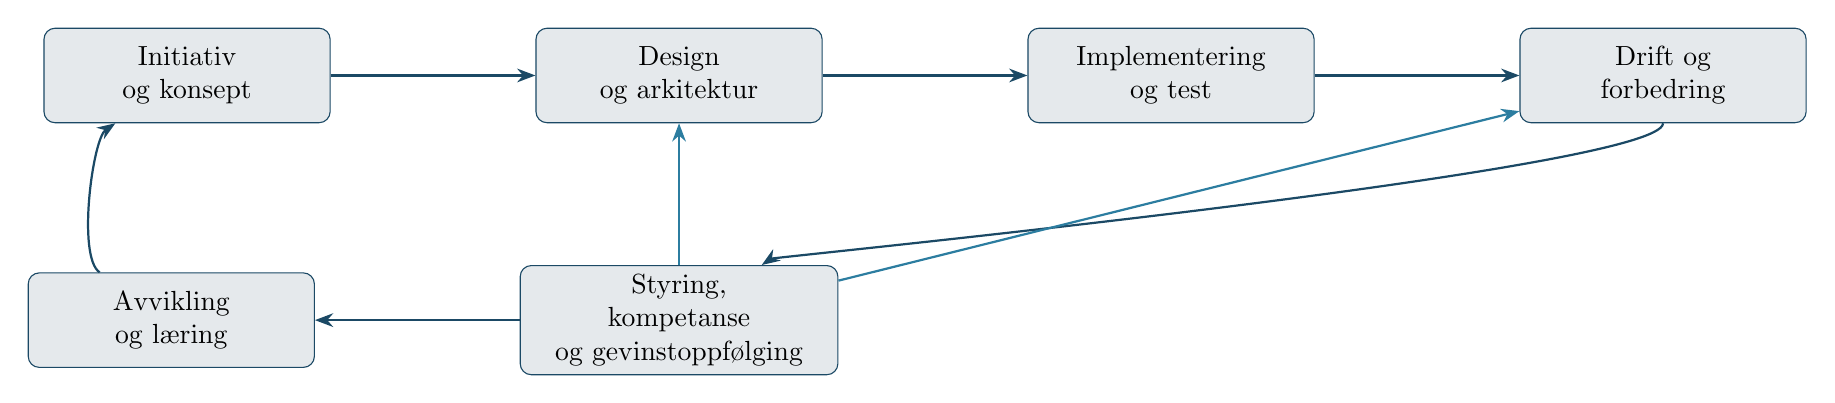
\begin{tikzpicture}[node distance=2.6cm, every node/.style={rectangle, rounded corners, draw=dypblaa, fill=skygraa, text width=3.4cm, align=center, minimum height=1.2cm}]
        \node (init) {Initiativ\\og konsept};
        \node[right=of init] (design) {Design\\og arkitektur};
        \node[right=of design] (implement) {Implementering\\og test};
        \node[right=of implement] (operate) {Drift og\\forbedring};
        \node[below=1.8cm of design, text width=3.8cm] (govern) {Styring,\\kompetanse\\og gevinstoppfølging};
        \node[left=of govern] (retire) {Avvikling\\og læring};
        \draw[->,>=Stealth,thick,dypblaa] (init) -- (design);
        \draw[->,>=Stealth,thick,dypblaa] (design) -- (implement);
        \draw[->,>=Stealth,thick,dypblaa] (implement) -- (operate);
        \draw[->,>=Stealth,thick,dypblaa] (operate) .. controls +(0,-1.2) and +(1.2,0.8) .. (govern);
        \draw[->,>=Stealth,thick,dypblaa] (govern) -- (retire);
        \draw[->,>=Stealth,thick,dypblaa] (retire) .. controls +(-1.2,0.8) and +(-1.2,-0.8) .. (init);
        \draw[->,>=Stealth,thick,petrol] (govern) -- (design);
        \draw[->,>=Stealth,thick,petrol] (govern) -- (operate);
    \end{tikzpicture}
    \caption{Livssyklusrammeverket som brukes i fagfelleløpet viser hvordan styring og læring kobles til fasene i \autoref{tab:raci-maritim}.}
    \label{fig:livssyklusramme}
\end{figure}

\section{Organisering og roller}
Styringen av digitale tvillinger krever en tydelig governance-modell som balanserer sentral koordinering og lokal innovasjon. Mange virksomheter etablerer et kjerneteam som forvalter plattformen, mens forretningsområder eller prosjektteam bygger spesifikke tvillinger på toppen.

\subsection*{Governance-modeller}
\begin{itemize}
    \item \textbf{Sentralisert modell:} Et dedikert «Center of Excellence» setter standarder, sikrer kompetanse og eier budsjett for tvillingplattformen. Passer godt i regulerte sektorer som energi og helse.
    \item \textbf{Føderert modell:} Domeneenheter eier sine tvillinger, men deler felles retningslinjer for data, sikkerhet og arkitektur. Et strategisk forum koordinerer veikart og prioriteringer.
    \item \textbf{Produktlinjemodell:} Tverrfaglige produktteam får ansvar for hele livssyklusen til en digital tvilling, inkludert finansiering og resultatmål. Plattformteam leverer felles komponenter og DevOps-støtte.
\end{itemize}

Tabell~\ref{tab:governance-sammenligning} sammenligner modellene på beslutningsfora, finansiering og egnethet. Oversikten brukes i workshops for å hjelpe virksomheter å vurdere hvilken struktur som passer deres modenhetsnivå.

\subsection*{Hybrid styring og utviklingssløyfer}
Selv om modellene beskrives separat, opplever mange virksomheter behov for en hybrid tilnærming. Et praktisk mønster er å etablere et sentralisert kjerneteam som definerer felles standarder, mens produktteam eier gevinstansvar. Det gir tre utviklingssløyfer som kan brukes i styringsdokumenter:
\begin{enumerate}
    \item \textbf{Strategisk sløyfe:} kvartalsvise portefølgemøter der konsernledelse, sikkerhetsansvarlige og produktteam samordner veikart og investeringer.
    \item \textbf{Taktisk sløyfe:} månedlige governance-forum der dataspace-råd, arkitektur og DevOps koordinerer endringsforslag og kvalitetskrav.
    \item \textbf{Operativ sløyfe:} ukevise standups med drift, domeneeksperter og læringsansvarlige som oppdaterer gevinstlogg og håndterer hendelser.
\end{enumerate}
Ved å tydeliggjøre hvilke beslutninger som tas i hver sløyfe, kan organisasjonen dokumentere ansvarslinjer i RACI-matrisen og justere ressursbehov etter modenhet.

\begin{table}[h]
    \centering
    \caption{Sammenligning av governance-modeller for digitale tvillinger}
    \label{tab:governance-sammenligning}
    \begin{tabular}{p{2.9cm}p{3.2cm}p{3.2cm}p{3.5cm}}
        \toprule
        Modell & Beslutningsfora & Finansiering & Typiske norske eksempler \\
        \midrule
        Sentralisert & Konsernråd for teknologi og sikkerhet & Sentralt investeringsbudsjett med felles gevinstplan & Statnetts nettplanleggingsprogram og Equinors Johan Sverdrup-plattform\citep{statnett2023digital,equinor2021johansverdrup} \\
        Føderert & Domenevise porteføljestyrer og dataspace-råd & Kostnadsdeling mellom virksomhetsområder etter bruk & Statsbyggs ombruksprogram og bytvillingen i Sluppen\citep{statsbygg2023loopfront,trondheim2024bytvilling} \\
        Produktlinje & Tverrfaglige produktteam med sprintdemoer & Produktteam eier resultatansvar, plattformteam fakturerer tjenester & Hydro CIRCALs materialsporingsprogram og Kognitwin-piloter i prosessindustri\citep{hydro2023traceability,kongsberg2023kognitwin} \\
        \bottomrule
    \end{tabular}
\end{table}

\subsection*{Rollefordeling og samhandling}
Produkteier, domeneekspert, data scientist, simuleringsspesialist og IT-drift må samarbeide tett. Rolleavklaringen bør konkretiseres gjennom en RACI-matrise som beskriver hvem som er ansvarlig (Responsible), beslutningstaker (Accountable), rådgiver (Consulted) og informert (Informed). Tabell~\ref{tab:raci-maritim} viser et eksempel for et maritimt vedlikeholdsprosjekt.

\begin{table}[h]
    \centering
    \caption{Eksempel på RACI-matrise for digital tvilling i maritimt vedlikehold}
    \label{tab:raci-maritim}
    \begin{tabular}{p{4cm}cccc}
        \toprule
        Aktivitet & Teknisk sjef & Produkteier & Data scientist & Skipsoffiser \\
        \midrule
        Definere vedlikeholdsstrategi & A & R & C & C \\
        Etablere datainnsamling & C & A & R & I \\
        Utvikle prediktiv modell & I & C & R & C \\
        Validere modell i drift & C & A & R & R \\
        Rapportere gevinster & R & A & C & I \\
        \bottomrule
    \end{tabular}
\end{table}

Eksterne leverandører bør inkluderes med klare kontrakter for ansvar og dataeierskap. Juridiske vurderinger må sikre at deling av sanntidsdata skjer i tråd med avtaler og regelverk.

\subsection*{RACI-variant for tverrsektorielle partnerskap}
Kryss-sektorielle initiativ, for eksempel batteriverdikjeder eller havvindplattformer, krever ofte at flere linjeorganisasjoner deler ansvar. En utvidet RACI-variant med kategorien \emph{Support} gjør det tydelig hvem som leverer operative ressurser selv om beslutningsmyndigheten ligger hos andre aktører. Tabell~\ref{tab:raci-variant} viser hvordan modellen kan anvendes på et dataspace-program der kommune, industri og teknologipartnere samarbeider.

\begin{table}[h]
    \centering
    \caption{RACI-S-matrise for dataspace-program i regionalt havvindinitiativ}
    \label{tab:raci-variant}
    \begin{tabular}{p{4.3cm}ccccc}
        \toprule
        Aktivitet & Kommune & Operatør & Plattformleverandør & Faglig rådgiver & TSO \\
        \midrule
        Fastsette delingspolicy og tilgangsnivå & A & C & R & C & I \\
        Implementere dataspace-kontrakter og API-er & I & C & R & C & S \\
        Overvåke datakvalitet og hendelser & C & R & S & C & A \\
        Planlegge vedlikeholdsvinduer & I & A & C & R & S \\
        Rapportere gevinster og bærekraftindikatorer & R & A & C & C & I \\
        \bottomrule
    \end{tabular}
\end{table}

Denne varianten forbereder leseren på å bruke malen i Appendiks~\ref{appendix:ressurser} der en generell tabell for RACI-S kan fylles ut for egne case.

\subsection*{Dataspace-governance og eskaleringslinjer}
Dataspace-samarbeid stiller krav til hvordan organisasjoner deler data, håndhever kontrakter og håndterer avvik. \citet{idsa2023ram} og \citet{gaiax2023architecture} beskriver hvordan noder må sertifiseres og hvordan tiltrode rollemyndigheter skal følge opp dataspace-policyer. Norske initiativ for mobilitet og energi legger til grunn at forvaltningsmodellen kombinerer tekniske komponenter (connectors, kataloger) med et styringsforum som kan sette bindinger for bruksvilkår.\citep{ec2023mobilitydataspace} For at kapittel 3 og 7 skal henge sammen i undervisningen, må studentene se hvordan dataspace-governance speiler de organisatoriske modellene over.

En praktisk måte å etablere styringen på er å definere fire beslutningsnivåer:
\begin{enumerate}
    \item \textbf{Strategisk råd:} Godkjenner dataspace-mandat, medlemskap og sanksjoner. Rådet eies gjerne av et offentlig-privat partnerskap hvor programleder for tvillinginitiativet sitter sammen med dataspace-operatør.
    \item \textbf{Operasjonelt forum:} Koordinerer onboarding, datakataloger og hendelser. Her deltar plattformteam, dataspace-arkitekter og juridiske rådgivere som vurderer datakontrakter mot \citet{digdir2023modelljournal}.
    \item \textbf{Domenegrupper:} Sektorspesifikke arbeidsgrupper (for eksempel helseteknologi eller mobilitet) som prioriterer data- og modellbehov, kvalitetssikrer semantikk og harmoniserer indikatorer fra Kapittel~6.
    \item \textbf{Eskaleringsteam:} Hurtigrespons-team med representanter fra sikkerhet, personvern og forretningssiden som kan pause deling eller oppdatere tilgangsvilkår ved avvik.
\end{enumerate}

Tabell~\ref{tab:dataspace-governance} viser hvordan styringsnivåene kan knyttes til konkrete artefakter og eskaleringspunkter i et regionalt dataspace-program. Oversikten kan brukes i casearbeid sammen med RACI-S-malen.

\begin{table}[h]
    \centering
    \caption{Styringsartefakter og eskalering i et regionalt dataspace-program}
    \label{tab:dataspace-governance}
    \begin{tabular}{p{3.2cm}p{4.2cm}p{4.2cm}p{3.0cm}}
        \toprule
        Beslutningsnivå & Hovedartefakt & Ansvarlige roller & Eskaleringspunkt \\
        \midrule
        Strategisk råd & Partnerskapsavtale med krav til sertifisering, medlemskap og gevinstplan & Programleder, kommuneadministrasjon, industripartnere & Revisjon mot dataspace-policy hvert halvår \\
        Operasjonelt forum & Datakatalog, tilgangspolicy og teknisk driftsrapport & Plattformteam, dataspace-arkitekt, juridisk rådgiver & Hendelser i connector eller uautorisert bruk \\
        Domenegrupper & Modelljournaler, semantiske vokabular og KPI-sett & Fagansvarlige, produktledere, data steward & Konflikt i datakvalitet eller indikatorer mellom sektorer \\
        Eskaleringsteam & Hendelseslogg, tilsynsrapport og beslutningslogg & Sikkerhetsleder, personvernombud, forretningsansvarlig & Pause eller stanse datadeling, varsling til tilsyn \citep{ec2023mobilitydataspace} \\
        \bottomrule
    \end{tabular}
\end{table}

Når artefaktene forvaltes i samme versjonskontroll som tvillingmodeller og datakataloger, blir det lettere å dokumentere etterlevelse av \citet{gaiax2023architecture} og å spore hvilke beslutninger som utløste endringer. Studentene bør kombinere tabellen med gevinstplanen under for å vise hvordan dataspace-governance støtter gevinstrealisering.

\subsection*{Gevinstplan og KPI-styring}
For å sikre kontinuerlig oppfølging bør kapittelteamet bruke en gevinstplan som kobler indikatorer til ansvarlige roller og beslutningsarenaer. Tabell~\ref{tab:gevinstplan} gir et eksempel på hvordan livssyklusfaser, KPI-er og datakilder kan organiseres. Malen speiler strukturen i Appendiks~\ref{appendix:ressurser} og kan tilpasses ulike sektorer.

\begin{table}[h]
    \centering
    \caption{Eksempel på gevinstplan for digital tvilling}
    \label{tab:gevinstplan}
    \begin{tabular}{p{2.8cm}p{3.8cm}p{3.5cm}p{3.2cm}}
        \toprule
        Livssyklusfase & Hovedindikator & Datakilde & Beslutningsarena \\
        \midrule
        Initiativ & Forventet netto nåverdi og modenhetsgrad & Forretningscase, vurderingsmatrise (Kapittel~8) & Porteføljestyre (kvartalsvis) \\
        Implementering & Sprintleveranser fullført og modellnøyaktighet & DevOps-rapporter, modellvalidering (Kapittel~6) & Styringsgruppe (hver sprint) \\
        Drift & Oppetid, datakvalitet og sikkerhetshendelser & Observabilitetsdashbord, hendelseslogger & Operasjonelt forum (ukentlig) \\
        Forbedring & Realiserte gevinster og læringspunkter & KPI-rapport, retrospektiver & Programstyre (månedlig) \\
        Avvikling & Dokumentert arv og gjenbruk & Arkiverte modeller, dataspace-policy & Kunnskapsforum (etterprosjekt) \\
        \bottomrule
    \end{tabular}
\end{table}

Ved å oppdatere gevinstplanen etter hver milepæl blir det lettere å holde oversikt over forutsetninger som må oppdateres når nye caser legges inn i undervisningen.

\subsection*{Bærekraft- og modenhetsindikatorer per sektor}
Livssyklusstyring må også følge opp klima- og ressursmål. Tabell~\ref{tab:baerekraft-kpi} gir eksempler på indikatorer fra tre sektorer som brukes i norske pilotprosjekter. De kompletterer gevinstplanen ved å vise hvordan bærekraftdata hentes og forankres i styringen.

\begin{table}[h]
    \centering
    \caption{Eksempler på bærekraft-KPI-er i norske digital-tvillingprosjekter}
    \label{tab:baerekraft-kpi}
    \begin{tabular}{p{2.9cm}p{3.6cm}p{3.2cm}p{3.3cm}}
        \toprule
        Sektor & Bærekraft-KPI & Datakilde & Formål \\
        \midrule
        Havvind & CO$_2$-intensitet per levert MWh og turbin-tilgjengelighet & Kombinerte driftssensorer og energibalanser fra Hywind Tampen & Dokumentere klimaeffekt og pålitelighet i samsvar med NVE-krav\citep{equinor2023hywindtampen,nve2023havvindfakta} \\
        Bygg og eiendom & Andel komponenter til gjenbruk samt avfallsreduksjon & BIM-modeller og Loopfront-logg for ombruk & Understøtte klimabudsjett og sirkulærøkonomistrategi hos Statsbygg\citep{statsbygg2023loopfront,regjeringen2021sirkulaer} \\
        Batteriverdikjede & Resirkuleringsgrad og energiforbruk per celle & Produksjonsdata fra Giga Arctic og leverandørsertifikater & Verifisere bærekraftskrav i støtteordninger og kundekontrakter\citep{freyr2024giga,enova2023batteri} \\
        \bottomrule
    \end{tabular}
\end{table}

Indikatorene brukes som utgangspunkt når studentene utvikler egne KPI-sett og kobler dem til dataspace-arkitekturen i \autoref{tab:governance-sammenligning}.

\subsection*{Modenhetssteg for bærekraftstyring}
For å knytte indikatorene til livssyklusen kan kapittelteamet bruke en trestegs modenhetsmodell. Den gjør det enklere å beskrive ambisjonsnivå i plan- og statusfiler og å følge opp tiltak i fagfellelogg:
\begin{enumerate}
    \item \textbf{Baseline:} Sektorteam registrerer grunnleggende klima- og ressursdata og kobler dem til ansvarlige roller i RACI-matrisen.
    \item \textbf{Integrert:} Bærekraft-KPI-er inngår i gevinstplan og beslutningsfora; dataspace-kontrakter sikrer deling med partnere.
    \item \textbf{Revisjonsklar:} Indikatorene revideres eksternt, støttes av sporbare dataprodukter og brukes i scenarioplanlegging for neste generasjon tvillinger.
\end{enumerate}
Modellen brukes som sjekkliste når nye case legges til i kapittel~\ref{chap:case} og når støttefilene oppdateres med krav til dokumentasjon.

\subsection*{Sirkulærøkonomisk gevinststyring}
Norske virksomheter forventes å dokumentere hvordan digitale tvillinger støtter ombruk, materialeffektivitet og klimaambisjoner.\citep{norskindustri2023sirkular,regjeringen2021sirkulaer} For å gjøre dette operativt bør gevinstplanen kobles til et sett med sirkulærøkonomiske indikatorer som følger tvillingen gjennom livssyklusen. Indikatorene må forankres i de samme beslutningsforaene som håndterer investeringer og dataspace-governance, slik at tiltakene prioriteres sammen med øvrige endringer.

Et praktisk oppsett for masterstudenter består av tre komponenter:
\begin{enumerate}
    \item \textbf{Material- og energiindikatorer:} Registrer gjenbrukbar andel, resirkuleringsgrad og energiforbruk per leveranse slik Statsbygg og Hydro gjør i sine tvillingprogram.\citep{statsbygg2022ombruk,hydro2023traceability}
    \item \textbf{Prosessindikatorer:} Følg opp hvor raskt komponenter flyttes gjennom sirkulære sløyfer og hvor mange beslutninger som er dokumentert i kontrolltårn eller fagfellelogg.
    \item \textbf{Resultatindikatorer:} Mål klimanytte, reduserte innkjøpskostnader og etterlevelse av offentlige krav, og del tallene i de samme gevinstmøtene som rapporterer økonomisk effekt.
\end{enumerate}

Tabell~\ref{tab:sirkular-livssyklus} viser hvordan indikatorene kan organiseres per fase og hvilke kilder som brukes. Strukturen speiler datastrømmene i kapittel~3 og gjør det tydelig hvem som eier målingene.

\begin{table}[h]
    \centering
    \caption{Sirkulærøkonomiske indikatorer gjennom livssyklusen}
    \label{tab:sirkular-livssyklus}
    \begin{tabular}{p{2.7cm}p{3.7cm}p{3.5cm}p{3.0cm}}
        \toprule
        Fase & Fokusområde & KPI og terskel & Datakilde/ansvar \\
        \midrule
        Initiativ & Sirkulær forretningscase & Potensiell ombruksandel $>30\%$ og CO$_2$-besparelse per år & Forretningsanalyse, livsløpsberegning (Kapittel~3) ledet av bærekraftsansvarlig \\
        Design & Material- og dataarkitektur & Fullstendig komponentregister og sporbarhetsplan & BIM/dataspace-kontrakter, modelljournal forvaltes av arkitekt \\
        Implementering & Operative sløyfer & Tid fra demontering til gjenbruk $<6$ uker, kvalitetssjekk i sandkasse & IoT-logger, kontrolltårnrapport (Kapittel~6) eid av operasjonsteam \\
        Drift & Kontinuerlig måling & Andel sirkulære leveranser per måned, energiforbruk per enhet & Observabilitetsdashbord og ERP-data, rapportert av produktteam \\
        Forbedring/avvikling & Læring og dokumentasjon & Dokumenterte læringspunkter og oppdaterte policyer innen 4 uker & Fagfellelogg, gevinstmøte og arkivansvarlig \\
        \bottomrule
    \end{tabular}
\end{table}

Når tabellen brukes i casearbeid, bør studentene samtidig oppdatere ressursbanken i appendikset med datasett og verktøy som støtter indikatorene. Dette sikrer at sirkulærøkonomi blir en integrert del av gevinststyringen og ikke et separat sideprosjekt.

\subsection*{Dataspace-arkitektur for styring og deling}
Livssyklusforvaltning i større økosystem krever en dataspace-arkitektur som definerer ansvar for dataprodukter, identitet og policy. En anbefalt struktur følger fire lag:
\begin{enumerate}
    \item \textbf{Dataprodukter og semantikk:} Domeneeiere beskriver datastrømmer med felles ordlister og metadata slik at partnere kan oppdage dem. Semantiske modeller gjør det mulig å koble tvillingen til dataspace-kontrakter.\citep{idsa2023ram}
    \item \textbf{Tillitstjenester:} Identitet, tilgangskontroll og policy-håndhevelse sørger for at bare autoriserte aktører får tilgang til sensitive data. Gaia-X nav og nasjonale forvaltere kan fungere som tillitsanker.\citep{gaiax2023architecture}
    \item \textbf{Edge og sky:} Data behandles så nær kilden som mulig for å sikre respons, mens aggregerte datasett lagres i sky for analyse og deling. Edge-noder må støtte samme sikkerhetskrav som sentrale plattformer.\citep{etsi2023mec}
    \item \textbf{Styringsfora:} Tverrfaglige råd følger opp avvik, oppdaterer gevinstplanen og prioriterer forbedringer. Output fra rådene dokumenteres i læringssløyfer (retrospektiver, fagfellelogg) slik at gevinstene kan revideres.
\end{enumerate}
Arkitekturen sikrer at gevinstplaner, RACI-matriser og modellforvaltning er koblet sammen gjennom felles dataprodukter og policyer.

\subsection*{Porteføljestyring og beslutningsporter}
Når flere digitale tvillinger inngår i samme program må ledelsen synliggjøre hvilke investeringer som gir størst effekt og når initiativ bør stoppes eller skaleres. En porteføljestyringsmodell samler gevinstplanen, dataspace-governance og læringssløyfene fra Kapittel~6 i et felles beslutningsforum.\citep{digdir2022gevinst,rcn2024digitalisering} Modellen gjør det mulig å prioritere mellom sektorer, balansere risiko og sikre at modne tvillinger får ressurser til videreutvikling.

Porteføljen styres gjennom fire hovedporter som dekker hele livssyklusen:
\begin{enumerate}
    \item \textbf{Port 0 – Idéutvelgelse:} vurderer strategisk verdi, data- og partnergrunnlag samt mulige koblinger til eksisterende dataspace-initiativ.
    \item \textbf{Port 1 – Pilotering:} beslutter finansiering av laboratorieløp og evaluerer regulatoriske forpliktelser før data deles.
    \item \textbf{Port 2 – Skalering:} kvalitetssikrer operasjonelle indikatorer, integrasjoner og gevinstplan før løsningen rulles ut bredt.
    \item \textbf{Port 3 – Drift og fornyelse:} følger opp realiserte gevinster, teknisk gjeld og beslutninger om videre investering eller avvikling.
\end{enumerate}

Tabell~\ref{tab:portefolje-porter} viser hvilke indikatorer og dokumenter som bør være klare ved hver port. Oversikten brukes i undervisningen for å koble fagteamene sine caseoppgaver til styringsarenaene i \autoref{tab:dataspace-governance} og gevinstplanen i Tabell~\ref{tab:gevinstplan}.

\begin{table}[h]
    \centering
    \caption{Beslutningsporter i porteføljen for digitale tvillingprogram}
    \label{tab:portefolje-porter}
    \begin{tabular}{p{2.8cm}p{3.8cm}p{3.4cm}p{3.4cm}}
        \toprule
        Port & Beslutningsfokus & Nøkkelindikatorer & Obligatoriske leveranser \\
        \midrule
        Port 0 – Idéutvelgelse & Strategisk relevans, datatilgang og partnerkapasitet & Forventet netto nytte, modenhetsanalyse og tilgangen til kritiske datasett & Hypotesekart, interessentoversikt og vurdering av dataspace-krav \\
        Port 1 – Pilotering & Gjennomføringskraft og regulatorisk klarering & Testplan, personvernrisiko og tilgangsklarering fra dataspace-forum & Laboratorieplan, sikkerhetsvurdering og beslutning om felles plattformressurser \\
        Port 2 – Skalering & Operasjonell robusthet og gevinstpotensial & Modellnøyaktighet, driftsindikatorer og gevinstplan med KPI-er & Integrasjonsarkitektur, kvalitetsjournal og oppdatert gevinstplan \\
        Port 3 – Drift og fornyelse & Gevinstrealisering, teknisk gjeld og videre investeringsbehov & Leveransegrad, revisjonsfunn og målt bærekraftseffekt & Oppdatert tiltakslogg, beslutning om videre finansiering og plan for neste iterasjon \\
        \bottomrule
    \end{tabular}
\end{table}

\subsection*{Tiltakslogg for gevinstoppfølging}
Etter hver porteføljebeslutning må tiltak dokumenteres slik at gevinstplanen faktisk gjennomføres. \citet{digdir2022gevinst} anbefaler å bruke en felles tiltakslogg der funn fra fagfellelogg, kvalitetsjournal og gevinstmøter knyttes til ansvarlige roller og tidsfrister. Når loggen forvaltes i samme repositorium som modelljournalen og dataspace-policyene, kan styringsgruppene lett sammenligne fremdrift på tvers av kapittel 3, 6 og 8.\citep{rcn2024digitalisering}

Tabell~\ref{tab:tiltakslogg} viser et forslag til struktur. Den kombinerer indikatorer fra Kapittel~6 med caseoppgaver fra Kapittel~8 og gjør det tydelig hvilke tiltak som må følges opp i neste gevinstmøte.

\begin{table}[h]
    \centering
    \caption{Eksempel på tiltakslogg for gevinstoppfølging}
    \label{tab:tiltakslogg}
    \begin{tabular}{|p{3.0cm}|p{4.0cm}|p{3.4cm}|p{2.5cm}|p{3.1cm}|}
        \hline
        \textbf{Tiltak} & \textbf{Utløsende funn} & \textbf{Ansvar} & \textbf{Frist} & \textbf{Oppfølging} \\n        \hline
        Oppdatere dataspace-kontrakt for mobilitetscase & Avvik i hendelsesjournalen for kollektivstresstest \citep{ruter2024mobilitetslab,vegvesen2023beredskap} & Programleder mobilitetstvilling + dataspace-arkitekt & 2 uker & Rapporteres i operativt forum og logges i kontrolltårn-panelet \\n        \hline
        Justere indikatorpanel for kommunal overvåking & Nye terskelverdier fra kapittel 6 sin månedsrapport \citep{oslo2023overvann,dsb2022beredskap} & Kommunal beredskapsleder + data steward & Neste månedsmøte & Verifiseres i tiltakslogg og fagfellelogg før neste øvelse \\n        \hline
        Utvide gevinstanalyse for sirkulær leverandørpakke & Revisjonsfunn om manglende klimaeffekt i leverandørstyring \citep{statsbygg2023loopfront,hydro2023traceability} & Kapittelredaktør Kapittel 7 + innkjøpsrådgiver & Kvartalsvis porteføljemøte & Resultatet føres i gevinstplan og deles med styringsforum \citep{dfo2024kontraktsoppfolging} \\n        \hline
    \end{tabular}
\end{table}

For å holde loggen aktuell bør kapittelteamet følge tre rutiner:
\begin{enumerate}
    \item \textbf{Synkroniser datakilder:} Eksporter indikatorer fra Kapittel~6 og caserapporter fra Kapittel~8 før gevinstmøtene, og knytt dem til tiltaksnummer i loggen.
    \item \textbf{Fordel ansvar:} Bruk RACI- og RACI-S-matrisene i dette kapittelet for å bekrefte hvem som er ansvarlig, beslutningstaker og støtteressurs for hvert tiltak.
    \item \textbf{Lukk tiltak strukturert:} Når tiltak er levert, oppdateres loggen med målt effekt, referanse til fagfellelogg og lenke til justert gevinstplan slik at porteføljestyret kan verifisere resultatet.
\end{enumerate}

Masterstudentene kan bruke loggen som mal i prosjektarbeid. Hver gruppe dokumenterer tiltak fra sine caseverksteder, legger ved indikatorresultater og reflekterer over hvordan tiltakene påvirker styrings- og dataspace-modellene som beskrives i dette kapittelet.

For kapittelteamet er porteføljestyringen en sjekkliste: Når en port er passert skal indikatorer og dokumenter oppdateres i planfilene og fagfelleloggen. Resultatene deles med programleder, slik at porteføljen rebalanseres i takt med nye case fra Kapittel~\ref{chap:case} og forskningsløpene i Kapittel~9.

\section{Leverandørstyring og anskaffelser}
Digital tvilling-initiativ kombinerer ofte interne utviklingsressurser med leveranser fra konsulenter, programvarehus og drifts-
partnere. For å sikre at gevinst- og kvalitetsmål oppnås må anskaffelser og kontrakter speile livssyklusmodellen i dette kapittelet.
\citet{dfo2023anskaffelser} anbefaler at behov og modenhet kartlegges i forkant av konkurranser, mens \citet{dfo2024kontraktsoppfolging}
viser hvordan kontraktsoppfølging bør kobles til styringsdata og gevinstplaner. Norske virksomheter som Bane NOR og Statsbygg
benytter i økende grad partnerskap og standardiserte ytelsesindikatorer for å sikre kontinuerlig leveranse av modelloppdateringer
og dataforvaltning.\citep{statsbygg2023digitalmodenhet,banenor2024leverandor}

\subsection*{Anskaffelsesløp for tvillingprogram}
Et strukturert anskaffelsesløp bør kombinere innovasjonspartnerskap, modulbaserte kontrakter og tydelige krav til datadeling.
Tabell~\ref{tab:anskaffelseslop} viser et eksempel på faser, leveranser og styringspunkter.

\begin{table}[h]
    \centering
    \caption{Eksempel på anskaffelsesløp for digital tvilling-program}
    \label{tab:anskaffelseslop}
    \begin{tabular}{|p{3.1cm}|p{4.6cm}|p{4.4cm}|p{3.0cm}|}
        \hline
        \textbf{Fase} & \textbf{Hovedleveranser} & \textbf{Tiltak og styring} & \textbf{Ansvarlig} \\
        \hline
        Behovsforberedelse & Modenhetsanalyse, gevinsthypoteser og datakartlegging & Workshop med fag og innkjøp, kobling til gevinstplanen og dataspace-krav fra Kapittel~3 & Programleder + innkjøpsrådgiver \\
        \hline
        Konkurransegjennomføring & Konkurransegrunnlag, tildelingskriterier og evalueringspanel & Bruk modningskrav fra \citet{dfo2023anskaffelser}, vurder leverandørers evne til deling via dataspace og DevOps-støtte & Anskaffelsesleder + teknisk komité \\
        \hline
        Kontraktsinngåelse & Leveranseplan, datakontrakter og sikkerhetsbilag & Harmoniser kontraktsmaler med Kapittel~6 sitt kvalitets- og tilsynsregime, etabler felles modelljournal & Juridisk rådgiver + sikkerhetsleder \\
        \hline
        Pilot og skalering & Sprintplan, KPI-er og læringslogg & Følg opp indikatorer i Tabell~\ref{tab:gevinstplan}, benytt måleverktøyene fra \citet{dfo2024kontraktsoppfolging} & Produkteier + leverandørteam \\
        \hline
    \end{tabular}
\end{table}

Ved å koble konkurransegrunnlag og kontraktsvilkår til gevinstplan og dataspace-governance unngår virksomheten at leverandører leverer
isolerte komponenter uten integrasjon. En tydelig datakontrakt som beskriver API-er, semantikk og eierskap gjør det mulig å gjenbruke
artefakter i nye prosjekter.\citep{digdir2023modelljournal}

\subsection*{Kontraktsoppfølging og samarbeid}
I drifts- og forbedringsfasen må leverandører følges opp gjennom faste styringsmøter og indikatorpaneler. \citet{ks2023leverandor}
anbefaler å kombinere tjenestenivå (SLA), modenhetsmåling og gevinstsporing, mens \citet{dfo2024kontraktsoppfolging} viser hvordan
kontraktsdata kan kobles til digitale dashboards for løpende kontroll.

\begin{enumerate}
    \item \textbf{Etabler felles styringsforum:} Samle programleder, leverandørens prosjektleder og sikkerhets- og personvernansvarlige
    i månedlige møter som bruker indikatorene fra Kapittel~6 og 7.
    \item \textbf{Bruk læringssløyfer:} Registrer avvik, forbedringsforslag og innovasjonsmuligheter i en delt logg som knyttes til
    tiltaksplanen i \citet{ks2023leverandor}. Dette støtter kontinuerlig forbedring og gjør at erfaringer kan flyttes mellom kontrakter.
    \item \textbf{Aktiver gevinststyring:} Koble målt gevinsteffekt til finansieringsmodeller og porteføljestyring. Ved avvik
    skal kontraktsmekanismer som bonus/malus eller opsjoner brukes til å justere leveranser.
\end{enumerate}

Tabell~\ref{tab:leverandoroppfolging} gir et eksempel på indikatorer som binder sammen kontraktsoppfølging, leveransestatus og livssyklusen.

\begin{table}[h]
    \centering
    \caption{Indikatorer for leverandørstyring i digital tvilling-program}
    \label{tab:leverandoroppfolging}
    \begin{tabular}{|p{3.2cm}|p{4.5cm}|p{4.2cm}|p{3.0cm}|}
        \hline
        \textbf{Indikator} & \textbf{Datakilde} & \textbf{Tiltak ved avvik} & \textbf{Kobling i livssyklusen} \\
        \hline
        Leveransegrad per sprint & Sprintdemoer, modelljournal og kontraktslogg & Juster backlog og ressursbruk, aktiver kontraktsklausuler for forsinkelse & Implementering og drift \\
        \hline
        Datakvalitet og delingsstatus & Dataspace-kontroller, API-målinger og SLA-rapport & Initiér forbedringsplan, oppdater delingspolicy og eskaler til dataspace-råd & Drift og forbedring \\
        \hline
        Gevinstrealiseringsindeks & Gevinstplan, KPI-panel og økonomirapporter & Gjennomfør gevinstreview, revurder finansiering og beslutningsport & Porteføljestyring \\
        \hline
        Kompetanseoverføring & Kurslogg, fagfellelogg og opplæringsplan & Utvid læringsopplegg, juster krav til dokumentasjon og støtte & Endringsledelse og avvikling \\
        \hline
    \end{tabular}
\end{table}

Leverandørstyring må også inkludere exit-strategier slik at data og kode overføres tilbake til virksomheten ved kontraktsslutt. En
strukturert avslutning med revisjon av dokumentasjon, datalagring og tilgangsstyring gjør at erfaringer kan tas med inn i neste
anskaffelsesrunde og reduserer risikoen for leverandørbinding.

\section{Endringsledelse og modenhet}
Digital tvilling er en organisasjonsutvikling like mye som et teknisk prosjekt. Modenhet kan vurderes i nivåer fra ad hoc-initiativ til kontinuerlig forbedring der tvillingen er integrert i virksomhetsstyringen. En modenhetsmodell kan beskrive kriterier for styringsstruktur, datakvalitet, automatisering og kompetanse på hvert nivå.

Endringsledelse handler om å bygge forståelse for hvorfor tvillingen er viktig, sikre eierskap hos ledelse og fagmiljø, og investere i opplæring. Kommunikasjon bør være målrettet mot ulike interessenter: operatører trenger praktiske arbeidsprosesser, mens ledelsen trenger indikatorer som viser strategisk effekt.

\subsection*{Måleindikatorer for gevinstrealisering}
Gevinster må følges opp med både kvantitative og kvalitative indikatorer:
\begin{itemize}
    \item \textbf{Operasjonelle KPI-er:} reduksjon i uplanlagt nedetid, optimalisert energiforbruk, forbedret produksjonsutnyttelse.
    \item \textbf{Kvalitetsindikatorer:} forbedret modellnøyaktighet, raskere saksbehandling for endringer, færre sikkerhetshendelser knyttet til datadelingsfeil.
    \item \textbf{Lærings- og innovasjonsmål (OKR-er):} antall eksperimenter kjørt i tvillingen per kvartal, nye tjenester som lanseres basert på innsikt fra tvillingen, kompetanseløft i tverrfaglige team.
\end{itemize}
Indikatorene bør inngå i virksomhetens styringssystem, eksempelvis balansert målstyring eller kvartalsvise portefølgereview. For å sikre kontinuerlig forbedring kan teamet gjennomføre retrospektiv-møter der avvik analyseres og tiltak prioriteres.

\subsection*{Kompetansepakke for dataspace-governance}
Fagfellepanelet etterspurte en helhetlig kompetansepakke som støtter dataspace-governance gjennom hele endringsreisen. Programlederen bør kombinere klasseromsøkter, digitale mikrokurs og praksisnære øvelser slik at både tekniske og organisatoriske roller får nødvendig trygghet. \citet{digdir2022gevinst} anbefaler at gevinstplan, organisering og kommunikasjon kobles til en egen opplæringsplan, mens \citet{dssc2023skills} beskriver hvordan dataspace-team må bygge kompetanse på både policy og teknologi. Tabell~\ref{tab:kompetansepakke} viser et opplegg som kan integreres i lærerveiledningen og caseøktene i Kapittel~\ref{chap:case}.

\begin{table}[h]
    \centering
    \caption{Kompetansepakke for dataspace-governance}
    \label{tab:kompetansepakke}
    \begin{tabular}{p{2.7cm}p{4.0cm}p{3.6cm}p{3.2cm}}
        \toprule
        Modul & Læringsmål & Nøkkelinnhold & Praktisk leveranse \\
        \midrule
        Strategisk oversikt & Forstå partnerskapsmodell, gevinstmål og regulatoriske krav & Dataspace-roller, gevinstplanlegging, kobling til NIS2 og personvern & Presentasjon og gevinstkart fra workshop \\
        Operasjonell forvaltning & Implementere policy, datakatalog og hendelseslogg & Modelljournal, tilgangsstyring, kontrolltårn-prosesser & Konfigurert mal i prosjektverktøy og oppdatert RACI-S \\
        Teknisk forankring & Beherske connector-arkitektur og kvalitetsmålinger & Referansearkitektur, testmiljø, observabilitetsdashbord & Proof-of-concept med integrert kvalitets- og sikkerhetsvarsling \\
        Endringsledelse og kommunikasjon & Planlegge opplæring, måleeffekter og forankre endringer & Målgruppetilpasning, kommunikasjonsplan, gevinstoppfølging & Kommunikasjonsplan og læringslogg delt i fagfelleloggen \\
        \bottomrule
    \end{tabular}
\end{table}

Kompetansepakken følger modenhetsstegene over og kan fases inn i pilotundervisningen uke~4--6. Studentene kan fordele modulene mellom roller i caset og bruke fagfelleloggen til å dokumentere hvem som trenger oppfølging.

\subsection*{Kommunikasjonsplan for endringsreise}
Effektiv endringsledelse krever målrettet kommunikasjon til ulike interessenter gjennom hele dataspace-reisen. Planen i Tabell~\ref{tab:kommunikasjonsplan} fungerer som sjekkliste i planleggingsfasen og kan justeres for sektorvise behov. Den kombinerer informasjonskanaler, ansvar og budskap slik \citet{digdir2022gevinst} anbefaler i gevinstoppfølgingen, og legger inn læringsaktiviteter i tråd med anbefalingene fra \citet{dssc2023skills} om kompetansebygging.

\begin{table}[h]
    \centering
    \caption{Kommunikasjonsplan for dataspace-endringsreise}
    \label{tab:kommunikasjonsplan}
    \begin{tabular}{p{2.8cm}p{3.6cm}p{3.6cm}p{3.4cm}}
        \toprule
        Fase & Målgrupper & Budskap og materiell & Ansvar og kanal \\
        \midrule
        Før oppstart & Programstyre, nøkkelpartnere, fagforeninger & Forretningsmål, gevinsthypoteser, forventet involvering & Programleder via styringsråd og partnerskapsbrev \\
        Pilotering & Operasjonsteam, dataspace-arkitekter, juridisk støtte & Policykrav, tilgangsprosesser, pilotcase og datakvalitetsmålinger & Dataspace-forum og dedikerte arbeidsmøter ledet av forvalter \\
        Utrulling & Sluttbrukere, leverandører, sikkerhetsmiljø & Endringsstøtte, opplæringstilbud, sikkerhetsrutiner og støttekanaler & Kommunikasjonsteam gjennom intranett, webinar og spørretimer \\
        Etterlevelse & Fagfeller, tilsyn, prosjektkontor & Resultater, gevinstrapport, læringslogg og videre tiltak & Programleder og fagteam gjennom kvartalsrapport og læringsworkshop \\
        \bottomrule
    \end{tabular}
\end{table}

Planen bør oppdateres etter hver retrospektiv. Studentteam kan bruke strukturen til å forberede interessentkart og identifisere hvor kommunikasjonsgap vil bremse gevinstrealiseringen.

\section{Intervjuguide for governance-case}
Tilbakemeldinger fra fagfellepanelet ba oss konkretisere hvordan intervjuer og workshops skal gjennomføres når governance-modellene testes i pilotundervisningen. Intervjuguiden i notatet `support/notater/pilotundervisning-materiell.md` brukes som grunnlag, og kobles til livssyklusfigur~\ref{fig:livssyklusramme} slik at hvert spørsmål peker til riktig fase og ansvar.

En strukturert økt kan gjennomføres slik:
\begin{enumerate}
    \item \textbf{Innledning (5 minutter):} Presenter formålet med caset og hvilke leveranser som skal testes. Bekreft samtykke til notater og eventuell opptak.
    \item \textbf{Fasevis dypdykk (20 minutter):} Bruk figuren til å kartlegge hendelser, beslutningspunkter og støtteverktøy i fasene initiativ, design, implementering og drift. Noter tydelige ansvar og avhengigheter.
    \item \textbf{Styring og gevinstoppfølging (10 minutter):} Undersøk hvordan indikatorer, opplæring og beslutningsfora fungerer i praksis. Diskuter hvordan tiltakene skal dokumenteres i fagfelleloggen.
    \item \textbf{Avslutning (5 minutter):} Oppsummer foreslåtte tiltak, avklar hvem som følger dem opp og hvilke data som kan deles videre i undervisningen.
\end{enumerate}

Resultatene bør overføres til fagfelleloggen og planens tiltaksoversikt slik at vi kan spore hvilke endringer som kreves før neste revisjon. Intervjuene danner også grunnlag for refleksjonsoppgaver i pilotundervisningen uke~5 og 6.

\section{Refleksjonsspørsmål og øvinger}
\begin{enumerate}
    \item Bruk Tabell~\ref{tab:raci-maritim} som inspirasjon og tilpass en RACI-matrise til et eget case, for eksempel en digital tvilling for kraftnett eller helseutstyr.
    \item Utform et sett med KPI-er og OKR-er som gjør det mulig å følge opp både kortsiktige driftsgevinster og langsiktig innovasjon.
    \item Beskriv hvilke tiltak som kreves for å løfte en organisasjon fra pilotnivå til helhetlig integrasjon av digitale tvillinger, inkludert styring, kompetanse og teknologi.
\end{enumerate}

\chapter{Bruksområder og norske case}
\label{chap:case}

\section{Læringsmål}
\begin{itemize}
    \item Analysere variasjon i anvendelser av digitale tvillinger på tvers av sektorer.
    \item Kritisk evaluere norske case med hensyn til teknologi, organisasjon og gevinster.
    \item Overføre læring fra case til egne prosjekter.
\end{itemize}

\section{Industrisektoren}
Digitale tvillinger i norsk industri kobler ofte sammen komplekse produksjonslinjer, leverandørkjeder og energisystemer. Når du analyserer casene, bør du identifisere hvilke beslutningssituasjoner som styrer investeringen, og hvordan innsikten fra tvillingen brukes til både operativ og strategisk styring. Erfaringer fra Yara, Hydro og andre prosessaktører viser at kontinuerlig forbedring og vedlikehold er like sentralt som nye investeringer.

\subsection*{Prosessindustri og produksjon}
I ferrolegering, aluminium og batteriindustri ser vi digitale tvillinger som kombinerer sanntidsdata fra produksjonslinjene med simuleringer for å optimere varmebalanse, kjemiske prosesser og logistikk. Hydro Sunndal bruker for eksempel virtuelle modeller til å følge elektrolysecellene og planlegge vedlikehold før avvik oppstår. Ved å fylle ut casemalen kan du dokumentere hvordan datainnsamling fra sensorer, laboratorier og ERP-systemer kobles til modellene, og hvilke styringsparametre (for eksempel OEE og energibruk per enhet) som måles for å vise gevinst.

\subsection*{Energi og kraft}
Kraftbransjen kombinerer produksjonsdata, nettanalyser og markedssignaler for å sikre forsyningssikkerhet og bærekraft. Statnett utvikler digitale tvillinger av transmisjonsnettet for å planlegge vedlikehold og håndtere flaskehalser, mens Statkraft integrerer værdata og hydrologiske modeller for å optimalisere vannkraftmagasinene. Når du bruker malen på slike case, bør du beskrive hvordan datakilder som SCADA, værprognoser og regulatoriske krav påvirker modellene og beslutningsprosessene.

\subsection*{Maritim og offshore}
I maritim sektor kombinerer aktører som Equinor, Kongsberg Maritime og Ulstein simuleringer av skip og plattformer med sanntidsdata fra sensorer. Tvillingene brukes til å planlegge logistikk i Nordsjøen, forutse vedlikehold på subsea-utstyr og teste nye autonome funksjoner. Et godt utfylt case viser hvordan operasjonssentraler, kapteiner og tekniske team samarbeider rundt modellen, og hvordan tvillingen knyttes til sikkerhet og miljørapportering. Utforsk datakilder og planleggingsverktøy samlet i \autoref{sec:maritimressurser} for å beskrive logistikk, miljøforhold og regulatoriske krav i caseleveransene.

\paragraph{Autonome ferger i Trondheimsfjorden}
Pilotprosjektet rundt passasjerfergen \emph{Milliampere 2} demonstrerer hvordan autonome fartøy kan inngå i mobilitetsløsninger for norske byer og dokumenteres som en del av Trondheims satsing på nullutslippsmobilitet.\citep{ntnu2023milliampere2} FoU-programmet AutoFerry beskriver hvordan Zeabuz og forskningsmiljøene bygger tvillingen med modulære sensorer, simulatorer og styringssystemer som kan overføres til flere havner.\citep{sintef2024autoferry} Casebriefen i `support/notater/maritim-caseforberedelse.md` dokumenterer mål, datakilder og styringsstruktur og fungerer som startpunkt for å fylle casemalen. Oppgaven til studentene er å beskrive hvordan tvillingen binder sammen fartøyet, fjernoperatører og kommunens mobilitetsstyring, og hvilke regulatoriske rammer som gjelder for testtilatelser og beredskap.

\begin{itemize}
    \item Kartlegg sensorer og eksterne datakilder (MET-værdata, AIS-strømmer, havneinformasjon) og beskriv hvordan de strømmer inn i datasjøen og simulatorene.
    \item Forklar hvordan prosjektets governance fordeler ansvar mellom Zeabuz, Trondheim kommune og forskningspartnerne, og hvordan endringsrådet evaluerer nye autonome funksjoner.
    \item Definer KPI-er for punktlighet, energibruk og sikkerhetsrespons og knytt dem til læringsmålene i Kapittel~3 (dataflyt) og Kapittel~6 (tillit og etikk).
    \item Bruk vurderingsmatrisen i dette kapittelet til å sammenligne caset med andre maritime initiativer, og dokumenter funnene i fagfelleloggen slik at prioriteringen kan forankres.
\end{itemize}

Integrer gjerne en illustrasjon fra `support/illustrasjonsplan.md` som viser samspillet mellom fartøyet, fjernoperasjonssenteret og byens øvrige transportsystem. Dette gjør det lettere for lesere å forstå hvordan datastrømmene og beslutningssløyfene knyttes sammen i en urban, maritim kontekst.

\section{Prioriterte case for kommende fagfelleløp}
For å støtte fagfelleløpet prioriteres tre nye case som dekker norsk energiomlegging, grønn industri og landbruksmodernisering. Notatene i `support/notater/` utdyper datakilder, KPI-er og styringsmodeller slik at arbeidsgrupper kan forberede intervjuer og dokumentasjon.

\subsection*{Havvind – Sørlige Nordsjø II og Hywind Tampen}
Utbyggingen av flytende havvind gir et rikt læringsgrunnlag for digital tvilling. Statlige rammer for areal og nettilknytning kombineres med Equinors operasjonserfaring fra Hywind Tampen, der turbiner og kraftplattformer deler data for å balansere produksjon mot sokkelinstallasjoner.\citep{nve2023havvindfakta,equinor2023hywindtampen} Tvillingen må koordinere værprognoser, vedlikeholdslogistikk og energioppgjør i en delt dataspace mellom operatør, Statnett og tjenesteleverandører. Når studentgruppene fyller ut casemalen skal de beskrive hvordan produksjonsdata, SCADA-signaler og markedsinformasjon synkroniseres i hydrodynamiske modeller og energioptimering på tvers av plattformer og nettilknytning.

\begin{table}[h]
    \centering
    \caption{Nøkkelspor for casestudiet i havvind}
    \label{tab:havvind-spor}
    \begin{tabular}{p{3.5cm}p{8.5cm}}
        \toprule
        Fokusområde & Eksempler på spørsmål som skal besvares i casemalen \\
        \midrule
        Operasjonelle modeller & Hvordan oppdateres laster, vær og produksjonsprognoser i sanntid, og hvilke beslutningsdører (for eksempel daglig produksjonsmøte og ukentlig vedlikeholdsforum) bruker simuleringene? \\
        Energioppgjør og markeder & Hvilke datagrunnlag brukes for å beregne fleksibilitet mot sokkelinstallasjoner, og hvordan dokumenteres avregning og kostnadsdeling mellom aktører? \\
        Beredskap og HMS & Hvordan loggføres hendelser, barrierestyring og sikkerhetstiltak, og hvordan deles tilsynskrav med myndighetene? \\
        Dataspace-styring & Hvilke policy-artefakter fra Gaia-X eller IDSA brukes for å regulere tilgang til sensordata, og hvordan versjoneres dem for nye samarbeidspartnere? \\
        \bottomrule
    \end{tabular}
\end{table}

\begin{itemize}
    \item Kartlegg integrasjonspunktene mellom turbinsystemer, nettilknytning og sokkelinstallasjoner, og dokumenter hvordan datakvalitet sikres før modeller oppdateres.\citep{nve2023havvindfakta}
    \item Beskriv hvordan styringsstrukturen fordeler ansvar mellom operatør, myndigheter og leverandørkjede, og pek på beslutningsfora som må involveres før endringer godkjennes.
    \item Definer indikatorer for kapasitetsfaktor, HSE-observasjoner og tilgjengelighet per turbin, og lenk dem til gevinstplanen i Kapittel~7.
    \item Referer til ressurser i \autoref{appendix:ressurser} om energi- og offshoredata, og noter hvilke kilder som trengs for å fylle ut malen i \autoref{sec:case-maler-prioriterte-sektorer}.
\end{itemize}

\subsection*{Landbruk – Presisjonsjordbruk i Trøndelag}
Presisjonsjordbruket gir studentene innsikt i kombinasjonen av edge-prosessering og sentral analyse. Jord- og maskinsensorer prosesseres lokalt for å støtte autonome arbeidsoperasjoner, mens agronomiske beslutninger dokumenteres i felles datasett for rådgivere og forvaltning.\citep{nibio2023dataflyt,landbruksdir2023digitalisering,etsi2023mec} Caset viser hvordan data kan deles mellom gårdbruker, forskningsmiljø og kooperativ med klare policyer for gjenbruk av feltdata. Når casemalen fylles ut bør analysen omfatte agronomiske beslutningspunkter, maskinlogistikk og datasikkerhet slik at både operasjonell styring og bærekraftsmål blir transparente.

\begin{table}[h]
    \centering
    \caption{Datakilder og styringsaktiviteter i presisjonsjordbrukscaset}
    \label{tab:landbruk-datakilder}
    \begin{tabular}{p{3.5cm}p{8.5cm}}
        \toprule
        Datakategori & Eksempler og dokumentasjonskrav \\
        \midrule
        Sensor- og maskindata & Jordfuktighet, NDVI og maskintelemetri lagres lokalt (edge) før utsnitt lastes til datasjø; beskriv hvordan kalibrering og datakvalitet sikres i sesongen. \\
        Agronomiske beslutninger & Gjødselplan, vekstskifte og plantevern loggføres i felles rådgivningsportal; noter hvordan beslutninger forankres i samvirke eller rådgivningstjenester. \\
        Forvaltnings- og policykrav & Dokumenter hvordan datadeling møter krav fra Landbruksdirektoratet og personvernforordningen, inkludert samtykkeprosesser for deling av feltdata. \\
        Bærekraftsindikatorer & Forklar hvordan klimagassregnskap, jordhelse og vannforbruk beregnes, og hvilke indikatorer som rapporteres tilbake til finansierings- eller sertifiseringsordninger. \\
        \bottomrule
    \end{tabular}
\end{table}

\begin{itemize}
    \item Kartlegg beslutningsarenaer gjennom vekstsesongen (planlegging, utsåing, vekstoppfølging, innhøsting) og knytt databehov til hver hendelse.\citep{landbruksdir2023digitalisering}
    \item Beskriv hvordan edge-arkitekturen (for eksempel MEC-noder og traktorkontrollere) filtrerer data før de sendes til skyløsningen, og hvilke hendelser som krever manuell verifisering.\citep{etsi2023mec}
    \item Definer KPI-er for avlingsprognoser, ressursbruk og klimaeffekt, og koble dem til vurderingsmatrisen for modenhet i dette kapittelet.
    \item Sammenlign datastrømmer og verktøy med ressurskategoriene i \autoref{appendix:ressurser}, og bruk veiledningen i \autoref{sec:case-maler-prioriterte-sektorer} for å dokumentere læringspunkter til undervisning og fagfeller.
\end{itemize}

\subsection*{Batteriverdikjede – Giga Arctic i Mo i Rana}
Norsk batteriproduksjon kobler prosessindustri, energi og logistikk. FREYR Battery etablerer digitale tvillinger som følger råvarer, produksjonslinjer og energiforbruk for å oppfylle kravene i EUs batteriforordning og Enovas støtteordninger.\citep{freyr2024giga,enova2023batteri,gaiax2023architecture,eu2023batteryregulation} Dataspace-tilnærmingen gjør at leverandørkjeder kan dele karbondata og kvalitetsmålinger under strenge kontraktsregimer. Analyse av caset må vise hvordan tvillingen støtter rapportering mot bærekraftsindikatorer, samtidig som produksjonstakt og kvalitet optimaliseres i samspill med energisystemet i Mo Industripark.

\begin{table}[h]
    \centering
    \caption{Avklaringer som bør inngå i batterikaset}
    \label{tab:batteri-fokus}
    \begin{tabular}{p{3.6cm}p{8.4cm}}
        \toprule
        Tema & Beskrivelse av forventet dokumentasjon \\
        \midrule
        Material- og leverandørflyt & Spesifiser hvordan råvarer spores fra ankomst via produksjonslinjene til ferdige celler, og hvordan avvik håndteres i MES/ERP. \\
        Energi- og klimarapportering & Redegjør for koblingen til lokale energisystemer, fleksibilitetsavtaler og hvordan CO$_2$-intensitet rapporteres til kunder og myndigheter. \\
        Kvalitetslaboratorier & Beskriv hvordan laboratoriedata integreres i tvillingen for å justere prosesstyring og prediktivt vedlikehold. \\
        Dataspace og kontrakter & Dokumenter kontraktsmekanismer for deling av prosess- og karbondata, inkludert tilgangskontroll og revisjonspunkter. \\
        \bottomrule
    \end{tabular}
\end{table}

\begin{itemize}
    \item Kartlegg hvordan tvillingen understøtter regulatoriske rapporteringskrav i EUs batteriforordning og norske støtteprogrammer, og dokumenter hvilke indikatorer som må eksporteres fra plattformen.\citep{eu2023batteryregulation,enova2023batteri}
    \item Beskriv grensesnittet mellom produksjonsplanlegging, energistyring og logistikk, og angi hvor sanntidsdata må tilgjengeliggjøres for partnere i Mo Industripark.
    \item Vurder hvilke modeller (for eksempel energibalansesimulering, yield-analyse og kvalitetsprognoser) som bør prioriteres i casemalen for å gi undervisningsverdi.
    \item Sett gevinstmål opp mot indikatorene i vurderingsmatrisen og bruk malen i \autoref{sec:case-maler-prioriterte-sektorer} til å dokumentere læringsopplegg, risiko og neste steg.
\end{itemize}

\begin{table}[h]
    \centering
    \caption{Oversikt over prioriterte case og nøkkelindikatorer}
    \label{tab:prioriterte-case}
    \begin{tabular}{p{3.2cm}p{2.6cm}p{4.6cm}p{3.6cm}}
        \toprule
        Case & Sektor & Hovedindikatorer & Dataspace-fokus \\
        \midrule
        Sørlige Nordsjø II / Hywind Tampen & Havvind & Kapasitetsfaktor, planlagt vs. faktisk vedlikehold, HSE-observasjoner & Deling av produksjons- og værdata mellom operatør, TSO og offshore-partnere \\
        Presisjonsjordbruk i Trøndelag & Landbruk & Avlingsprognose, nitrogenutnyttelse, klimafotavtrykk per enhet & Samtykkebasert deling av feltdata og agronomiske anbefalinger mellom bønder og rådgivere \\
        Giga Arctic, Mo i Rana & Batteri & First-pass yield, energiforbruk per GWh, CO$_2$-intensitet per celle & Kontraktsstyrt tilgang til prosess-, logistikk- og bærekraftsdata i industrielt dataspace \\
        \bottomrule
    \end{tabular}
\end{table}

\subsection*{Felles leveranseplan for klimacaser}
Nasjonale satsinger som Grønt industriløft og de fremvoksende norske dataspace-pilotene viser at sektorenes klimaprosjekter må planlegges i fellesskap for å utløse investeringer og sikre datadeling på tvers av bransjer.\citep{regjeringen2023grontindustriloft,digitalnorway2024dataspace} For å gi fagfellegruppene en tydelig arbeidsflyt etableres en leveranseplan der havvind-, landbruks- og battericase har synkroniserte milepæler.

\begin{table}[h]
    \centering
    \caption{Leveranseplan for klimacase-workshop}
    \label{tab:klimacase-leveranser}
    \begin{tabular}{p{3.0cm}p{3.2cm}p{3.2cm}p{3.2cm}}
        \toprule
        Milepæl & Havvind & Landbruk & Batteri \\n        \midrule
        Forberedelse (uke $-2$) & Oppdater produksjons- og værdatasett, bekreft tilgang til Statnett og OED-notater. & Samle sesongplaner fra rådgivningstjenesten og jordprøver til datakvalitetssjekk. & Synkroniser prosesslogger og energidata med leverandørportalen i Mo Industripark. \\n        Workshopdag (uke 0) & Valider hydrodynamiske scenarier og beredskapsrutiner med fagfeller. & Test edge-arbeidsflyt og agronomisk beslutningslogg i sanntidsøkt. & Evaluer produksjonsdashbord mot krav i batteriforordningen og lokale fleksibilitetsavtaler. \\n        Oppfølging (uke $+1$) & Prioriter tiltak for dataspace-policy og publiser læringspunkter i fagfelleloggen. & Revider samtykkeprosesser og oppdater KPI-er for ressursbruk og klima. & Fastsett forbedringer i kvalitetslaboratorier og energisamarbeid før neste sprint. \\n        Skaleringsbeslutning (uke $+4$) & Beslutt om caset skal brukes i pilotundervisningen og hvilke modeller som gjenbrukes. & Bekreft hvilke gårder som inngår i videre utrulling og hvilke datasett som åpnes. & Avklar eksport av innsikt til verdikjeden og rapportering til Grønt industriløft. \\n        \bottomrule
    \end{tabular}
\end{table}

Bruk leveranseplanen i \autoref{tab:klimacase-leveranser} som agenda når fagfeller og studentgrupper møtes. Hver milepæl bør kobles til konkrete dokumenter i prosjektets samhandlingsrom (for eksempel casemaler, gevinstplaner og risikoanalyser) og til de ressursene som er listet i \autoref{appendix:ressurser}. Når planene følges, blir det enklere å gjenbruke beslutningsgrunnlag og sikre at datastrømmene er forankret i nasjonale politiske prioriteringer.

\begin{enumerate}
    \item Forankre leveranseplanen hos ansvarlige for kapittel 3 og 7 slik at dataspace-policy og gevinstoppfølging henger sammen i hele boken.
    \item Oppdater `support/notater/pilotundervisning-materiell.md` etter hver milepæl med status, kontaktpunkter og eventuelle avhengigheter mot illustrasjoner eller laboratorieoppsett.
    \item Del erfaringer i fagfelleloggen slik at neste revisjon av leveranseplanen kan bygge på konkrete innsikter fra norsk industri og offentlig sektor.
\end{enumerate}

Casebeskrivelsene bygger videre på casemalen i dette kapittelet og gevinstplanen i Kapittel~7. Sektorgruppene bør fylle ut notatmalene med intervjuer, datatilgang og planlagte figurer før fagfellemøtene.

\subsection*{Dataspace-arkitektur for sektorkase}
Casene over illustrerer hvordan dataspace-prinsipper kan gjøre deling tryggere og mer fleksibel. Start med å etablere dataprodukter (for eksempel værvinduer, gjødselplaner eller energirapporter) med tydelig lisens. Bruk standardiserte policy-rammeverk fra IDSA og Gaia-X for å modellere tilgang og forretningsregler, og koble dem til KPI-oppfølgingen.\citep{idsa2023ram,gaiax2023architecture} Resultatet dokumenteres i prosjektets gevinstplan og RACI-matriser, slik at undervisningscasene får en konsistent styringsstruktur.

\section{Bygg, transport og helse}
Offentlige og private aktører bruker digitale tvillinger til å koordinere investeringer og tjenester som påvirker hele samfunnet. Felles utfordringer er å forankre tvillingen i eksisterende forvaltningssystemer, sikre datadeling og bygge kompetanse på tvers av fagmiljøer. Casemalen hjelper deg med å tydeliggjøre roller og datakilder i prosjekter der mange interessenter må samarbeide.

\subsection*{Smarte bygg og byer}
Statsbygg, Oslo kommune og flere norske byer har tatt i bruk digitale modeller som kombinerer BIM-data med energi- og sensorinformasjon for å styre drift og vedlikehold. Ved å beskrive scope, datakilder og governance i casemalen kan du vise hvordan driftsteam, leietakere og tjenesteleverandører bruker tvillingen til å redusere energibruk, planlegge renhold og forbedre inneklima.

\subsection*{Transport og logistikk}
Bane NOR utvikler digitale tvillinger av jernbanenettet for å planlegge vedlikehold, simulere trafikkavvik og informere kundeservice. Avinor tester tilsvarende modeller på flyplasser for å koordinere bakketjenester. Når du analyserer slike case, må du kartlegge hvordan sanntidsdata fra sensorer, IoT-enheter og trafikkstyringssystemer flyter inn i tvillingen, og hvordan det støtter planlegging og krisehåndtering. Utforsk datakilder som Entur, Bane NOR og Avinor i \autoref{sec:transportressurser} for å sikre at caserapporter støttes av konkrete tidsserier, kapasitetsdata og hendelseslogger.

\subsection*{Kommunal klimaresiliens og beredskap}
Oslo VAV har etablert en digital tvilling av vann- og avløpsnettet som kombinerer hydrologiske modeller, sensordata og sanntidsvarsling for å planlegge tiltak mot styrtregn og overvann.\citep{oslovav2023digital} Tvillingen brukes sammen med kommunens overvannsstrategi for å teste konsekvenser av utbygginger, dimensjonere blågrønne tiltak og prioritere investeringer i kulverter og magasiner.\citep{oslo2023overvann} Ved å dokumentere caset kan studentene vise hvordan data fra værstasjoner, trykksensorer og manuelle inspeksjoner gir grunnlag for beslutninger i beredskapsstaber og tekniske etater.

\begin{table}[h]
    \centering
    \caption{Arbeidsflyt for beredskap mot styrtregn i kommunal digital tvilling}
    \label{tab:kommunal-beredskap}
    \begin{tabular}{p{3.4cm}p{4.5cm}p{5.0cm}}
        \toprule
        Fase & Kritiske datakilder & Typiske tiltak og beslutninger \\
        \midrule
        Forberedende analyser & Regnhendelsesstatistikk, kapasitetsmålinger i ledningsnett, planregister & Prioriterer fordrøyningsbasseng og grønne løsninger, oppdaterer investeringsplaner og byggesaker. \\
        Operativ beredskap & Sanntidsnivå i kummer, værvarsler, sensordata fra overløp & Aktiverer beredskapstropp, koordinerer innsats mellom vann- og avløpsvakt og bymiljøetat, varsler utsatte institusjoner. \\
        Etterarbeid og læring & Skadejournal, hendelsesrapport, øvelseslogg & Evaluerer tiltak i tråd med DSBs øvelsesveileder, oppdaterer tiltaksbank og deler læringspunkter i fagfelleloggen.\citep{dsb2024nser,dsb2023ovelser} \\
        \bottomrule
    \end{tabular}
\end{table}

Når casemalen fylles ut, bør du beskrive hvordan den kommunale tvillingen kobles til dataspace-prinsippene i kapittel~3 og valideringsrutiner i kapittel~6. Det innebærer å dokumentere hvilke dataprodukter som deles med nabokommuner eller statlige myndigheter, og hvordan tilgang styres under hendelser. Bruk tabellen i \autoref{tab:kommunal-beredskap} for å konkretisere hvem som tar hvilke beslutninger og hvordan indikatorer for responstid, overløpsutslipp og samfunnskritiske tjenester følges opp.

\begin{itemize}
    \item Kartlegg hvordan overvannstiltak prioriteres gjennom kommunens porteføljestyring, og lenk til gevinstplanene i kapittel~7 for å vise hvordan investeringsbeslutninger forankres politisk.
    \item Beskriv hvordan beredskapsøvelser og scenarioarbeid dokumenteres i kvalitetsjournaler, og referer til metodikken i kapittel~6 for å sikre sporbarhet i etterlevelse.
    \item Presenter forslag til undervisningsaktiviteter der studentgrupper simulerer styrtregnscenarier og foreslår kombinasjoner av tekniske og naturbaserte tiltak basert på tvillingens data.
\end{itemize}

\subsection*{Helse}
Helse Vest og Universitetssykehuset i Oslo eksperimenterer med pasientspesifikke tvillinger for kreftbehandling, kirurgisk planlegging og rehabilitering. Malen gir struktur for å beskrive hvordan kliniske data, bildediagnostikk og simuleringer integreres, hvilke etiske vurderinger som gjøres, og hvordan pasienter og fagpersonell involveres i beslutninger. I pilotcaset for virtuell pasientflyt kobles valideringsløpet til Helseplattformens kontinuitetsplan for å sikre at dataflyt, arbeidsprosesser og beredskap synkroniseres mellom sykehus og kommunale tjenester.\citep{helseplattformen2023kontinuitet}

En helsetvilling bygger på en nasjonal dataspace-arkitektur som muliggjør styrt tilgang til sanntidskapasitet, laboratorieresultater og pasientlogistikk uten å kompromittere personvernet.\citep{nhn2024dataspace} Når casemalen fylles ut bør du beskrive hvordan tvillingen overholder helseberedskapskrav, og hvordan kontrolltårnene for drift, pasientsikkerhet og forskning samarbeider.\citep{hod2020beredskap} Dokumentasjonen skal vise hvordan data fra kliniske kjernesystemer, digitale hjemmeoppfølgingstjenester og velferdsteknologi bindes sammen slik at pasientforløp og ressursdisponering kan simuleres.\citep{helsedir2020dho}

\begin{table}[h]
    \centering
    \caption{Kontrollpunkter for virtuell pasientflyt i helsetvilling}
    \label{tab:helse-pasientflyt}
    \begin{tabular}{p{3.4cm}p{4.7cm}p{4.6cm}}
        \toprule
        Fase & Kritiske datakilder & Kontrollspørsmål for styring \\
        \midrule
        Kapasitetsplanlegging & Operasjonsplaner, sengeposter, ventelister & Hvordan varsles endringer i kapasitet, og hvilke beslutningsfora håndterer eskalering? \\
        Klinisk koordinering & Kliniske kjernejournaler, laboratoriedata, beslutningsstøtte & Er algoritmene verifisert mot etisk komité og tredjepartskrav før anbefalinger tas i bruk?\citep{ehelse2024tilsyn} \\
        Beredskap og læring & Kontinuitetsplaner, hendelseslogger, opplæringsdata & Hvordan sikres internkontroll og etterlevelse av tilsynskrav etter hendelser eller øvelser?\citep{helsetilsynet2024internkontroll} \\
        \bottomrule
    \end{tabular}
\end{table}

\begin{itemize}
    \item Kartlegg datautveksling og tilgangspolicyer i dataspace-portalen, og dokumenter hvordan roller og samtykker forvaltes i tråd med Norm for informasjonssikkerhet.\citep{nhn2024dataspace,norm2023}
    \item Test caset mot beredskapsplanen og kontinuitetsrutinene slik at scenarier for massetilstrømming og nedetid kan simuleres før pilotundervisningen.\citep{hod2020beredskap,helseplattformen2023kontinuitet}
    \item Oppdater vurderingsnotatet med kontrollspørsmål fra veiledere for digital hjemmeoppfølging og tredjepartsvurdering, og koble funnene til Kapittel~6 sine valideringskrav.\citep{helsedir2020dho,ehelse2024tilsyn}
    \item Registrer forbedringstiltak i kvalitetsjournalen og fagfelleloggen slik at internkontrollen viser hvordan caset følger opp tilsyn og læring.\citep{helsetilsynet2024internkontroll}
\end{itemize}

\section{Metodikk for caseanalyse}
For å sammenligne case på tvers av sektorer, start med å beskrive hvorfor tvillingen ble etablert, hvilke forutsetninger som må være til stede og hvordan resultatene måles. Det kan være nyttig å kombinere casemalen med intervjuer, offentlige rapporter og tekniske arkitekturdokumenter. Et helhetlig rammeverk bør dekke mål, omfang, teknologivalg, organisering og dokumenterte effekter.

\begin{itemize}
    \item Kartlegg datakilder systematisk, fra sanntidssensorer til historiske arkiv og åpne data, og vurder kvalitet, eierskap og tilgang.
    \item Noter hvilke styringsstrukturer, insentiver og kompetanseprogram som påvirker gjennomføring og skalering.
    \item Reflekter over etiske og samfunnsmessige hensyn, inkludert personvern, arbeidstakerperspektiv og miljøpåvirkning.
\end{itemize}

\subsection{Prioritering for pilotundervisningen}
Fagfelleinnspillene fra Statnett, Equinor og Helse Vest anbefalte at vi velger et begrenset sett case til pilotundervisningen slik at studentene kan fordype seg i datastrømmer og styringsprosesser. Prioriteringen nedenfor bygger på vurderingsmatrisen og de datadelingstiltakene som er tilgjengelige gjennom Gaia-X og norske dataspace-initiativer.\citep{gaiax2022architecture} Oversikten dokumenteres også i `support/notater/pilotundervisning-materiell.md` slik at mentorene har oppdaterte kontaktpunkter og lisenskrav.

\begin{table}[htbp]
    \centering
    \begin{tabular}{p{3.2cm}p{2.2cm}p{4.5cm}p{4.5cm}}
        \toprule
        \textbf{Case} & \textbf{Prioritet} & \textbf{Datastrømmer} & \textbf{Tiltak fra fagfelleløpet} \\
        \midrule
        Autonome ferger (Trondheim) & Høy & AIS, værdata, operativ logg, sikkerhetsrapporter & Datasett deles via kommunens dataspace; intervjuguide for fjernoperasjon oppdatert med sikkerhetsindikatorer. \\
        Kraftnett i Nord-Norge & Høy & SCADA, flaskehalsmodellering, energimarked & Avklarte tilgang til Statnetts sandkasse; tiltak for beredskap og NIS2-rapportering dokumentert. \\
        Batteriproduksjon Mo i Rana & Middels & MES, energi- og logistikkdata, kvalitetsmålinger & Datasamarbeid med industriparkens datasjø; plan for syntetiske datasett der produksjonsdata er sensitive. \\
        Virtuell pasientflyt (Helse Vest) & Middels & Kliniske registre, ressursplanlegging, ventelistestatistikk & Tidsluker for pseudonymisering av data avtalt; etikk- og samtykkestrømmer koblet til Kapittel~6. \\
        Smarte bygg (Oslo kommune) & Utforsk & Energi- og inneklimadata, arbeidsordre & Pilot holdes i reserve; krever videre avklaringer om deling via kommunal dataspace. \\
        \bottomrule
    \end{tabular}
    \caption{Prioritert caseliste for pilotundervisningen basert på fagfelleinnspill og tilgjengelige datastrømmer.}
\end{table}

\subsection*{Vurderingsmatrise for modenhet og prioritering}
Når flere potensielle case konkurrerer om oppmerksomhet eller undervisningsressurser, kan en vurderingsmatrise gi et felles
beslutningsgrunnlag. Tabellen under brukes til å skåre hvert case fra~1 (lav modenhet) til~5 (høy modenhet) på fem dimensjoner.
Noter begrunnelsen for hver skår og lenk til dokumentasjon, slik at fagfeller kan etterprøve vurderingen.

\begin{longtable}{p{0.23\textwidth}p{0.26\textwidth}p{0.45\textwidth}}
\toprule
\textbf{Kriterium} & \textbf{Hva vurderes?} & \textbf{Eksempel på skåringsskala (1--5)} \\
\midrule
\endfirsthead
\toprule
\textbf{Kriterium} & \textbf{Hva vurderes?} & \textbf{Eksempel på skåringsskala (1--5)} \\
\midrule
\endhead
Datagrunnlag og tilgang & Tilgjengelighet, kvalitet og rettigheter til data som trengs for tvillingen. & 1~= fragmenterte kilder uten tilgangsavklaringer. 3~= etablerte datastrømmer, men mangler kvalitetssikring. 5~= sanntidsdata med avtalte API-er, eierskap og datakvalitetsrutiner. \\
\addlinespace
Organisatorisk forankring & Hvor godt case er støttet av ledelse, fagmiljø og brukere. & 1~= initiativ fra enkeltperson uten mandat. 3~= prosjektgruppe med midlertidig finansiering. 5~= tverrfaglig styringsmodell med dedikerte roller og gevinstansvar. \\
\addlinespace
Teknologisk modenhet & Modenhet på modeller, integrasjonsplattform og driftsoppsett. & 1~= konseptskisse uten implementert plattform. 3~= pilot i begrenset produksjon. 5~= robust løsning med DevOps-/MLOps-sløyfer og overvåkning i drift. \\
\addlinespace
Gevinst- og læringspotensial & Forventet effekt for virksomheten og læringsverdi for studenter. & 1~= uklare mål og lite overføringsverdi. 3~= tydelige KPI-er, men begrenset dokumentasjon. 5~= målbare gevinster, åpne data/artefakter og tydelig kobling til læringsmål. \\
\addlinespace
Risiko og etterlevelse & Regulatoriske, sikkerhets- og etiske forutsetninger. & 1~= ukjente krav eller høy personvernrisiko. 3~= identifiserte tiltak, men ufullstendig dokumentasjon. 5~= komplette risikovurderinger, etterlevelsesplan og jevnlig revisjon. \\
\bottomrule
\end{longtable}

Etter at tabellen er fylt ut, summeres skårene for et samlet modenhetsnivå, men noter også hvordan svakheter skal håndteres.
Følg denne arbeidsflyten for å forankre prioriteringen:

\begin{enumerate}
    \item Sett sammen et tverrfaglig vurderingsteam (for eksempel produktansvarlig, dataarkitekt og domeneekspert) og avklar
    hva slags beslutning som skal tas.
    \item Innhent nødvendig dokumentasjon: prosjektmandat, tekniske beskrivelser, datalister og gevinstrealiseringsplaner. Bruk
    ressursoversikten i \autoref{appendix:ressurser} for å finne støttedata eller verktøy som mangler.
    \item Skår casene i fellesskap, dokumenter begrunnelser og registrer resultatet i prosjektets styrings- eller fagfellelogg.
    \item Definer tiltak for kriterier som får skår 1--2 (for eksempel avklare tilgang, etablere governance eller komplettere
    risikovurdering) og gi tydelig anbefaling om case skal prioriteres, videreutvikles eller settes på vent.
\end{enumerate}

Ved å dele vurderingsmatrisen med studenter og eksterne samarbeidspartnere blir det lettere å diskutere hvilke case som gir mest
verdi, og hvilke forberedelser som kreves før data kan deles eller modeller kobles på.

\section{Casestudie-maler for prioriterte sektorer}
\label{sec:case-maler-prioriterte-sektorer}
Denne seksjonen gir tre casemaler som speiler prioriteringene i \S~«Prioriterte case for kommende fagfelleløp». Hver mal beskriver hvilke spørsmål som skal besvares, hvilke datakilder som må dokumenteres og hvordan gevinstplanen fra Kapittel~7 kan kobles på.

\subsection{Havvind – Sørlige Nordsjø II og Hywind Tampen}
\paragraph{Sammendrag av caset}
\begin{tabular}{p{0.34\textwidth}p{0.60\textwidth}}
\textbf{Element} & \textbf{Beskrivelse / spørsmål som skal besvares} \\
Operatør og lokasjon & Hvilke selskaper deltar i tvillingen, og hvordan er havområdet delt mellom aktørene? \\
Strategiske mål & Hvordan balanseres energi til sokkelinstallasjoner mot eksport til fastlandet, og hvilke klimamål skal støttes? \\
Omfang & Hvilke anlegg og tjenester inngår (turbiner, kabler, substasjoner, logistikkfartøy)? \\
Utgangspunkt & Hvilke modeller, datakilder og driftserfaringer fantes før caset ble utvidet til en helhetlig tvilling? \\
\end{tabular}

\paragraph{Forretningsmål og interessenter}
\begin{itemize}
    \item Beskriv hvordan operatør, lisenspartnere, Statnett og leverandører bruker tvillingen til å koordinere produksjon, fleksibilitet og kraftpriser.\citep{nve2023havvindfakta}
    \item Identifiser relevante myndigheter (OED, NVE, Petroleumstilsynet) og hvilke krav til miljørapportering og HMS som tvillingen må støtte.
    \item Definer KPI-er for kapasitetsfaktor, vedlikeholdstid, CO$_2$-reduksjon og leveringssikkerhet.
\end{itemize}

\paragraph{Datagrunnlag og integrasjon}
\begin{itemize}
    \item Kartlegg SCADA-data, metocean-modeller, inspeksjonsrapporter og markedsdata, og forklar hvordan de samles i dataspace og kontrollrom.\citep{gaiax2023architecture}
    \item Dokumenter grensesnitt mot sokkelinstallasjoner, hydrodynamiske simuleringer og kraftmarkedsplattformer.
    \item Vurder hvordan datastrømmer kvalitetssikres før beslutninger fattes (for eksempel validering mot værbojer og inspeksjonsdroner).
\end{itemize}

\paragraph{Modelleringsstrategi}
\begin{itemize}
    \item Beskriv bruk av vær- og produksjonsprognoser, lastflytanalyse og strukturelle modeller av turbin og fundament.
    \item Forklar hvordan modellene kalibreres, og hvilke scenarioer som simuleres (storm, nettilkobling, vedlikeholdsvinduer).
    \item Angi hvordan beslutninger loggføres slik at modellforbedringer kan spores.
\end{itemize}

\paragraph{Implementering og arbeidsprosesser}
\begin{itemize}
    \item Forklar hvordan tvillingen støtter daglige operasjoner (for eksempel operations centre dashboards, vedlikeholdsplanlegging og energioppgjør).
    \item Beskriv opplæring for driftsteam, leverandørkjede og myndighetsdialog.
    \item Noter hvordan policy-artefakter og tilgangsstyring vedlikeholdes i dataspace-portalen.\citep{gaiax2023architecture}
\end{itemize}

\paragraph{Resultater, gevinster og gevinstrealisering}
\begin{itemize}
    \item Dokumenter gevinstmål for energiproduksjon, tidsbesparelse i vedlikehold og redusert nedetid.
    \item Beskriv hvordan gevinster verifiseres gjennom produksjons- og HMS-rapporter.
    \item Vurder sekundære effekter, som bedre sameksistens med fiskeri og skipsfart eller raskere konsesjonsoppfølging.
\end{itemize}

\paragraph{Overføringsverdi og neste steg}
\begin{itemize}
    \item Drøft hvordan modeller og datainnsikt kan gjenbrukes i nye felt (for eksempel Utsira Nord) eller andre offshoreprosjekter.
    \item Foreslå tiltak for å koble tvillingen til handelsplattformer og beredskapsøvelser.
    \item Identifiser beslutningspunkter for skalering til internasjonale partnere og testing av nye turbintyper.
\end{itemize}

\subsection{Landbruk – Presisjonsjordbruk i Trøndelag}
\paragraph{Sammendrag av caset}
\begin{tabular}{p{0.34\textwidth}p{0.60\textwidth}}
\textbf{Element} & \textbf{Beskrivelse / spørsmål som skal besvares} \\
Gård og produksjon & Hvilke produksjoner inngår (korn, gras, potet) og hvor ligger gården? \\
Strategiske mål & Skal tvillingen optimalisere avling, ressursbruk, klima eller dyrevelferd? \\
Omfang & Hvilke maskiner, sensorer og agronomiske beslutninger er inkludert? \\
Utgangspunkt & Hvilke digitale verktøy og datakilder fantes før presisjonsprogrammet startet? \\
\end{tabular}

\paragraph{Forretningsmål og interessenter}
\begin{itemize}
    \item Beskriv målene til bonden, rådgivningstjenesten, samvirket og eventuelle forskningspartnere.\citep{landbruksdir2023digitalisering}
    \item Avklar hvordan finansieringsordninger og sertifiseringer påvirker prioriteringer.
    \item Definer KPI-er for avlingsprognoser, inputfaktorbruk og klimafotavtrykk.
\end{itemize}

\paragraph{Datagrunnlag og integrasjon}
\begin{itemize}
    \item Kartlegg sensorer (jord, vær, maskinlogg), datasiloer (FMIS, ERP) og eksterne kilder (satellitt, rådgiving).\citep{nibio2023dataflyt}
    \item Beskriv edge-arkitekturen: hvilke data behandles lokalt, hvilke sendes til sky og når kreves offline-funksjonalitet?\citep{etsi2023mec}
    \item Dokumenter samtykke- og delingsprosesser for data mot rådgivere, leverandører og myndigheter.
\end{itemize}

\paragraph{Modelleringsstrategi}
\begin{itemize}
    \item Forklar hvilke modeller som kombineres (vekstmodeller, maskinlogistikk, agronomiske beslutningsstøtter).
    \item Angi hvordan modeller kalibreres mot jordprøver, avlingsdata og forsøksfelt.
    \item Beskriv hvordan usikkerhet og værvariasjon håndteres i anbefalinger.
\end{itemize}

\paragraph{Implementering og arbeidsprosesser}
\begin{itemize}
    \item Dokumenter hvordan tvillingen brukes i vekstsesongens beslutningspunkter og hvem som godkjenner tiltak.
    \item Beskriv opplæring og støtte for driftslag, inkludert digitale arbeidsflyter for maskinoperatører.
    \item Noter hvordan datakvalitet og datasikkerhet følges opp i samarbeidet med leverandører.
\end{itemize}

\paragraph{Resultater, gevinster og gevinstrealisering}
\begin{itemize}
    \item Oppgi målbare effekter for avling, innsatsfaktorer, klima og jordhelse.
    \item Beskriv hvordan resultatene dokumenteres (for eksempel i rådgivningsportal eller bærekraftsregnskap).
    \item Vurder sekundære gevinster som kompetanseheving og datadeling mot agronomi- og innovasjonsprosjekter.
\end{itemize}

\paragraph{Overføringsverdi og neste steg}
\begin{itemize}
    \item Identifiser hvordan løsningene kan skaleres til andre regioner, klima eller produksjoner.
    \item Foreslå tiltak for å koble tvillingen til forsyningskjeder, finansiering og sensorinnovasjon.
    \item Beskriv indikatorer som viser når tvillingen er klar for å inngå i landsdekkende samarbeidsprosjekter.
\end{itemize}

\subsection{Batteriverdikjede – Giga Arctic i Mo i Rana}
\paragraph{Sammendrag av caset}
\begin{tabular}{p{0.34\textwidth}p{0.60\textwidth}}
\textbf{Element} & \textbf{Beskrivelse / spørsmål som skal besvares} \\
Virksomhet og lokasjon & Hvilke anlegg og partnere inngår i Mo Industripark? \\
Strategisk hovedmål & Hvordan skal tvillingen støtte oppskalering, kvalitet og bærekraft? \\
Omfang & Hvilke produksjonslinjer, laboratorier og logistikkprosesser er inkludert? \\
Utgangspunkt & Hvilke systemer og datakilder fantes før Giga Arctic-programmet ble igangsatt? \\
\end{tabular}

\paragraph{Forretningsmål og interessenter}
\begin{itemize}
    \item Beskriv målbildet til FREYR Battery, energiselskap, logistikkpartnere og offentlige virkemidler.\citep{freyr2024giga,enova2023batteri}
    \item Angi hvordan kundenes krav til karbonavtrykk og kvalitet styrer prioriteringer.
    \item Definer KPI-er for produksjonskapasitet, first-pass yield, energibruk og CO$_2$-intensitet.
\end{itemize}

\paragraph{Datagrunnlag og integrasjon}
\begin{itemize}
    \item Kartlegg datakilder i råvarelogistikk, produksjonslinjer, laboratorier, energisystem og forsyningskjede.
    \item Beskriv integrasjoner mellom OT-systemer (OPC UA, PLC) og datasjø/analyseløsninger, samt hvordan data deles i dataspace.\citep{gaiax2023architecture}
    \item Dokumenter krav fra EUs batteriforordning og norske støtteprogrammer til rapportering og sporbarhet.\citep{eu2023batteryregulation,enova2023batteri}
\end{itemize}

\paragraph{Modelleringsstrategi}
\begin{itemize}
    \item Forklar hvordan prosessimulering, energibalansesimulering og kvalitetsprognoser kombineres.
    \item Beskriv kalibrering mot laboratoriedata og produksjonsstatistikk, samt håndtering av usikkerhet i nye produksjonsserier.
    \item Vurder behov for AI-modeller i produksjonsoptimalisering og vedlikehold.
\end{itemize}

\paragraph{Implementering og arbeidsprosesser}
\begin{itemize}
    \item Dokumenter hvordan tvillingen brukes i daglig drift, kvalitetsstyring og samarbeid med energipartnere.
    \item Beskriv opplæringsprogrammer for operatører, dataanalytikere og leverandører.
    \item Forklar hvordan versjonsstyring, datasikkerhet og revisjoner gjennomføres i dataspace og styringsmodeller.
\end{itemize}

\paragraph{Resultater, gevinster og gevinstrealisering}
\begin{itemize}
    \item Oppgi gevinster for energioptimalisering, yield, vedlikehold og bærekraftsrapportering.
    \item Beskriv hvordan gevinster dokumenteres gjennom interne dashboards og rapportering til myndigheter og kunder.
    \item Noter sekundære effekter som kompetanseheving, industrisamarbeid og nye forretningsmodeller.
\end{itemize}

\paragraph{Overføringsverdi og neste steg}
\begin{itemize}
    \item Vurder hvordan løsningen kan gjenbrukes i andre batteriprosjekter eller prosessindustrier.
    \item Definer tiltak for å koble tvillingen til europeiske dataspace-initiativer og leverandørkjeder.
    \item Foreslå indikatorer for når tvillingen bør utvides med nye produktlinjer eller geografiske lokasjoner.
\end{itemize}

\subsection*{Felles sjekkliste for caserapporten}
\begin{itemize}
    \item[$\square$] Er mål, interessenter og scope tydelig dokumentert med kobling til gevinstplanen?
    \item[$\square$] Er datakilder, integrasjoner og dataspace-policyer beskrevet med ansvar og kvalitetstiltak?
    \item[$\square$] Er modelleringsvalg, kalibrering og scenarioer forklart med tilhørende begrensninger?
    \item[$\square$] Er arbeidsprosesser, opplæring og governance definert med tydelige roller?
    \item[$\square$] Er gevinster og målemetoder forankret i KPI-er og vurderingsmatrisen?
    \item[$\square$] Er læringspunkter og neste steg formulert slik at fagfeller kan følge opp?
\end{itemize}

\subsection*{Eksempler på norske casetilpasninger}
\paragraph{Digital tvilling av kraftnett i Nord-Norge}
Statnett og regionale nettselskaper samarbeider om å modellere flaskehalser i kraftnettet mellom Ofoten og Finnmark. Når en av malene i denne seksjonen brukes, bør du beskrive hvordan værdata, planlagte industrietableringer og driftsmønstre fra vann- og vindkraft integreres, og hvordan tvillingen støtter dialogen med NVE og lokalsamfunn.

\paragraph{Jernbanedrift og vedlikehold hos Bane NOR}
En digital tvilling av jernbanestrekningen mellom Oslo og Lillehammer kombinerer BIM-modeller, sensordata fra spor og sanntidssignaler fra togene. Malstrukturen hjelper deg å dokumentere hvordan operasjonssentralen, entreprenører og leverandører samarbeider om vedlikeholdsvinduer og hvordan simuleringer brukes til å planlegge nye ruteoppsett.

\paragraph{Virtuell pasientflyt i spesialisthelsetjenesten}
Helse Sør-Øst prøver ut digitale tvillinger for å koordinere pasientflyt i kreftbehandling. Malen tydeliggjør hvilke kliniske datasett som inngår, hvordan algoritmer foreslår behandlingsplaner og hvordan pasienter får informasjon. Etisk vurdering, datasikkerhet og samtykkeprosesser må dokumenteres grundig.

\section{Refleksjonsspørsmål og øvinger}
\begin{enumerate}
    \item \textbf{Analyse av eksisterende case:} Velg ett av caseeksemplene ovenfor eller et eget norsk prosjekt. Bruk casemalene i \autoref{sec:case-maler-prioriterte-sektorer} til å skrive en kort rapport (2--3 sider) der du vurderer modenhet, måloppnåelse og hvilke ytterligere datakilder som kan styrke tvillingen.
    \item \textbf{Planlegging av nytt initiativ:} Sett sammen et tverrfaglig team (for eksempel prosessingeniør, data scientist og driftsleder) og lag et arbeidsnotat som beskriver hvordan dere vil samle data, utvikle modeller og organisere forvaltning for et nytt case i deres sektor ved å følge strukturen i \autoref{sec:case-maler-prioriterte-sektorer}.
    \item \textbf{Tverrsektoriell overføring:} Sammenlign to sektorer, for eksempel kraft og bygg. Lag en tabell som viser hvilke komponenter i casemalene som er direkte overførbare, hvilke som må tilpasses, og foreslå tiltak for å gjenbruke modeller eller datagrunnlag.
    \item \textbf{Refleksjon over etikk og verdiskaping:} Diskuter i grupper hvordan personvern, arbeidsmiljø og bærekraft bør ivaretas når tvillinger skaleres. Bruk notater fra de tre foregående oppgavene og oppdater relevante casemaler med konkrete risikoreduserende tiltak.
\end{enumerate}

\chapter{Fremtidstrender og forskning}

\section{Læringsmål}
\begin{itemize}
    \item Identifisere forskningsfronten innen digitale tvillinger.
    \item Diskutere fremtidige teknologier og samfunnsmessige konsekvenser.
    \item Formulere forskningsspørsmål og prosjektidéer.
\end{itemize}

\section{Forskningslandskapet}
Digitale tvillinger har etablert seg som et tverrfaglig forskningsfelt der systemteknikk, informatikk og domeneekspertise møtes. De mest synlige trendene springer ut av store internasjonale programmer som kobler akademia, leverandørindustri og offentlige aktører, samtidig som nasjonale prioriteringer legger føringer for hvilke problemstillinger som løftes frem i Norge.

\subsection{Internasjonale drivere}
EU har gjort digitale tvillinger til et kjerneelement i \emph{Horizon Europe} gjennom klynger som fokuserer på industriell digitalisering, energi og helseteknologi. Programmer som \emph{Destination Earth} og Gaia-X arbeider med felles dataplattformer og modeller for kritisk infrastruktur, og setter standarder som også påvirker norske miljøer. På forskningssiden markerer IEEE, ISO og Plattform Industrie 4.0 seg med veikart for interoperabilitet, semantikk og sikkerhet. Det gir en rik portefølje av referansemodeller, åpne datasett og calls for proposals som masterstudenter kan bruke som utgangspunkt for problemstillinger.

\subsection{Norske satsinger}
Forskningsrådet finansierer flere store miljøer, blant annet SFI Manufacturing, SFI Autoship og FME Neutron som alle utforsker digitale tvillinger i produksjon, maritime operasjoner og energi. Disse prosjektene kombinerer laboratorier, pilotanlegg og partnerskap med selskaper som Equinor, Kongsberg Gruppen, Elkem og offentlige etater. I tillegg gir regionale initiativ som katapultsentrene og Grønn plattform-prosjekter tilgang til testfasiliteter for masterstudenter. Norske kommuner og helseregioner stiller etter hvert krav om digitale tvillinger i anskaffelser, noe som åpner dører for anvendt forskning på mobilitet, helse og byggforvaltning.

\subsection{Forskningsinfrastruktur og testarenaer}
I løpet av de siste årene har norske universiteter, institutter og katapultmiljøer etablert felles laboratorier der digitale tvillinger kan testes i realistiske omgivelser. Slike arenaer gjør det lettere for masterstudenter å få tilgang til sensordata, produksjonsutstyr og simulatorer uten å forstyrre ordinær drift. SFI Manufacturing ved Raufoss Industripark kombinerer produksjonsceller, additiv tilvirkning og datainnsamling for å eksperimentere med sanntidsoptimalisering og bærekraftsmåling.\citep{sfi_manufacturing2023} Tilsvarende gir SFI Autoship tilgang til autonome testfartøy og kontrollrom som kan kobles til tvillingmodeller for logistikk og havnedrift.\citep{sfi_autoship2023}

Komplementære miljøer i Trondheimsfjorden og Oslofjorden tilbyr maritime og energirelaterte scenarioer. NTNU og SINTEF sitt OceanLab gjør det mulig å kombinere sensorer i fjorden, digitale simuleringsmodeller og fjernopererte fartøy for å teste sikkerhetskritiske beslutninger før de rulles ut i full skala.\citep{sintef2024oceanlab} Data Space Norway, koordinert av Digital Norway, fungerer som en samarbeidsarena der industripartnere, kommuner og forskere kan dele datasett og policy-komponenter for dataspace-baserte tvillinger.\citep{digitalnorway2024dataspace} For masterprosjekter betyr dette at prototyper kan valideres mot ekte datakilder, samtidig som juridiske og organisatoriske krav dokumenteres i samarbeid med laboratoriene.

Tabell~\ref{tab:testarenaer} viser et utdrag av infrastrukturer som er tilgjengelige for bokas målgruppe. Oversikten kan brukes til å planlegge feltarbeid, definere databehov og avklare hvilke støttefunksjoner (for eksempel sikkerhet, personvern og standardisering) som må involveres.

\begin{table}[h]
    \centering
    \caption{Utvalgte norske testarenaer for digitale tvillinger}
    \label{tab:testarenaer}
    \begin{tabular}{|p{3.2cm}|p{4.6cm}|p{4.4cm}|p{3.0cm}|}
        \hline
        \textbf{Infrastruktur} & \textbf{Faglig fokus} & \textbf{Tilgang for masterstudenter} & \textbf{Kontaktpunkt} \\n        \hline
        SFI Manufacturing Lab & Produksjonsoptimalisering, sirkulær materialflyt, prediktivt vedlikehold & Prosjektavtaler gjennom NTNU/HiØ; tilgang til produksjonsceller og datasett via sikkerhetsklarerte arbeidsstasjoner & SFI Manufacturing sekretariat \citep{sfi_manufacturing2023} \\n        \hline
        SFI Autoship Living Lab & Autonom navigasjon, logistikk, fjernoperasjon av fartøy & Pilotperioder med følgeforskning, fjernaksess til kontrollrom og sensorstrømmer ved avtalt veiledning & SFI Autoship prosjektledelse \citep{sfi_autoship2023} \\n        \hline
        OceanLab Trondheim & Havbruk, energiøyer og maritim beredskap med kombinasjon av fysiske testplattformer og digitale tvillinger & Bestillingsløp for laboratorietid, datalagring i sikker sky og bruk av fjernopererte farkoster & NTNU/SINTEF OceanLab koordinering \citep{sintef2024oceanlab} \\n        \hline
        Data Space Norway sandkasse & Dataspace-arkitektur, policy-automatisering og standardiserte konnektorer & Medlemskap via partnerorganisasjon gir tilgang til sandbox, connector-bibliotek og juridiske maler for datadeling & Digital Norway dataspace-team \citep{digitalnorway2024dataspace} \\n        \hline
    \end{tabular}
\end{table}

Når studentgrupper planlegger datainnsamling bør de kontakte laboratorienes fagansvarlige i forkant for å sikre at datasett og tilgangsavtaler er på plass. Erfaringer og målinger som gjøres i testarenaene bør dokumenteres i prosjektets kvalitetsjournal og knyttes til indikatorene i Tabell~\ref{tab:forskningsindikatorer}, slik at resultatene kan gjenbrukes i finansieringssøknader og fagfellevurderinger.

\subsection{Samarbeidsformer og metoder}
Feltet domineres av tverrfaglige metoder som kobler modellering, dataanalyse og brukerinnsikt. Levende laboratorier (living labs) og sandkasser gjør det mulig å eksperimentere med datatilgang, mens dataspaces og standardiserte API-er legger til rette for datadeling på tvers av virksomheter. Publikasjoner i tidsskrifter som \emph{Computers in Industry}, \emph{Advanced Engineering Informatics} og \emph{IEEE Access} viser en utvikling fra konseptstudier til empiriske evalueringer av driftseffekter og bærekraftsgevinster. En masterstudent bør derfor kombinere kvantitative indikatorer (for eksempel energi, kvalitet eller risiko) med kvalitative intervjuer som belyser organisering og beslutninger.

\section{Teknologitrender}
Teknologisk utvikling setter nye rammer for hva digitale tvillinger kan løse og hvordan de driftes. Det skjer en sammensmelting mellom simuleringsverdenen, sanntidsdata og intelligent beslutningsstøtte, noe som øker autonomien i både industrielle og samfunnsrettede systemer.

\subsection{Generativ AI og beslutningsassistenter}
Foundation-modeller og multimodale generative teknikker brukes nå til å foreslå designalternativer, generere syntetiske datasett og veilede operatører i komplekse beslutninger. Industripartnere eksperimenterer med copiloter som kombinerer naturlig språk, visualisering og historiske tvillingdata for å foreslå tiltak i sanntid.\citep{siemens2023copilot} Den europeiske AI-handlingsplanen fremhever behovet for ansvarlige, dokumenterte modeller, noe som innebærer at tvillinger må ha forklaringslag og revisjonsspor før generativ AI kan tas i bruk i regulerte bransjer.\citep{eu2023ai}

\subsection{Edge-native tvillinger}
For prosesser som krever lav responstid kombineres digitale tvillinger med edge-komponenter der databehandling skjer tett på utstyret. Standarder for multi-access edge computing gjør det mulig å orkestrere containere og AI-modeller i fabrikkhaller, på fartøy eller i landbruksmaskiner, samtidig som policyer for dataspace-tilgang ivaretas.\citep{etsi2023mec} Edge-native mønstre utfordrer tradisjonell skyarkitektur og krever at DevOps- og MLOps-prosesser inkluderer distribuerte oppdateringer, overvåking og fallback-rutiner.

\subsection{Semantiske tvillinger og autonomi}
De mest modne tvillingene bygger nå på semantiske modeller der kunnskapsgrafer og ontologier beskriver forholdet mellom komponenter, datastrømmer og forretningsregler. Kombinert med maskinlæring, probabilistiske modeller og formelle verifikasjonsmetoder gir dette grunnlag for beslutninger som kan automatiseres. Autonome tvillinger brukes til å orkestrere vedlikehold, balansere energinett og styre logistikksystemer, men krever transparens og sporbarhet slik at operatører kan forstå og overstyre kritiske valg.

\subsection{Immersive arbeidsflater og metaverset}
Utvidet virkelighet, digitale arbeidsrom og metaverse-plattformer gjør det mulig å visualisere komplekse systemer for operatører og borgere. Kombinasjonen av 3D-modeller, sanntidsstrømmer og samarbeidsverktøy lar tverrfaglige team samhandle om scenarioanalyse, opplæring og fjernoperasjon. Forskningen fokuserer på hvordan slike grensesnitt kan gi situasjonsforståelse uten å overbelaste brukeren, og hvordan sikkerhet og personvern ivaretas når data distribueres til mange enheter.

\subsection{Dataspace-økosystemer og samarbeid}
Europeiske dataspace-initiativer endrer hvordan virksomheter deler data og modeller. Gaia-X og IDSA legger til rette for at digitale tvillinger kan kobles på eksterne datastrømmer uten å gi fra seg kontroll over forretningshemmeligheter.\citep{gaiax2022architecture,idsa2023ram} For norske aktører betyr dette at energidata, maritime logistikkstrømmer eller helseinformasjon kan tilgjengeliggjøres gjennom standardiserte konnektorer, samtidig som tilgang styres av policyer og sertifisering. Forskningsfronten undersøker hvordan slike dataspace-plattformer kan kombineres med semantiske modeller og automatisert etterlevelse, slik at tvillinger kan forhandle om datadeling i sanntid og dokumentere hvilke regler som gjelder for hver transaksjon.

\section{Forskningsetikk, datahåndtering og åpen vitenskap}
Ambisiøse masterprosjekter må forholde seg til både juridiske krav, etiske vurderinger og forventninger om deling av resultater. Kravene kommer fra institusjonenes egne retningslinjer, personvernregelverket, finansieringskilder og fagfelleprosesser. En strukturert tilnærming gjør at forskningsaktivitetene kan dokumenteres, evalueres og gjenbrukes på tvers av kapitlene i denne boken.

\subsection{Personvern og forhåndsvurdering}
All bruk av personopplysninger, helseopplysninger eller andre sensitive data krever forhåndsvurdering og tydelig forankring hos dataansvarlig. Sikt tilbyr veiledning for hvordan behandlingsgrunnlag, dataminimering og informasjonssikkerhet skal dokumenteres før datainnsamlingen starter.\citep{sikt2023personvern} For medisinske og helsefaglige prosjekter må Regional komité for medisinsk og helsefaglig forskningsetikk (REK) involveres når prosjektet omfatter levende personer, biologisk materiale eller helsejournaler.\citep{rek2024forhandsvurdering} Den praktiske arbeidsflyten kan organiseres slik:
\begin{enumerate}
    \item \textbf{Kartlegg datakategorier:} Beskriv hvilke felt i datasettet som er personidentifiserende, og vurder behov for pseudonymisering eller anonymisering.
    \item \textbf{Definer ansvar og roller:} Etabler RACI-lister som kobler prosjektleder, veileder, personvernombud og eksterne partnere, slik Kapittel~7 anbefaler for styringsstrukturer.
    \item \textbf{Forbered godkjenningsløp:} Samle maler for samtykke, databehandleravtaler og REK-søknad i et eget prosjektarkiv slik at endringer kan spores i kvalitetsjournalen fra Kapittel~6.
\end{enumerate}

\subsection{Datahåndteringsplan og tilgangsstyring}
De fleste finansieringsprogram krever en oppdatert datahåndteringsplan (DMP) som viser hvordan data samles inn, lagres, deles og bevares. Norges forskningsråd stiller krav om at DMP-en dekker organisering, metadata, sikkerhet og eventuelle begrensninger for gjenbruk av data.\citep{forskningsradet2023aapen} Planen bør oppdateres når prosjektet beveger seg gjennom milepælene i finansieringstabellen lenger ned i kapitlet. Tabellen under viser hvordan tiltakene kan kobles til de øvrige kapittelene i boka.

\begin{table}[h]
    \centering
    \caption{Tiltak for ansvarlig håndtering av forskningsdata}
    \label{tab:forskningsdata-tiltak}
    \begin{tabular}{|p{3.2cm}|p{5.0cm}|p{4.2cm}|}
        \hline
        \textbf{Tiltak} & \textbf{Formål} & \textbf{Relaterte kapitler og verktøy} \\
        \hline
        Datahåndteringsplan & Dokumentere datakilder, lagring, tilgang og arkivering med versjonskontroll & Kapittel~3 (dataspace-policy), Kapittel~6 (kvalitetsjournal) \\
        \hline
        Tilgangsmatrise og sporbarhet & Sikre at bare autoriserte personer har tilgang, og at alle operasjoner logges & Kapittel~4 (simuleringsinfrastruktur), Kapittel~7 (governance og roller) \\
        \hline
        Plan for langtidsbevaring & Avklare hva som skal publiseres åpent, hva som skal lagres i institusjonelle arkiv og hvilke metadata som kreves & Kapittel~8 (casebank) og ressursappendiks \\
        \hline
    \end{tabular}
\end{table}

Når tiltakene er nedfelt i en DMP kan prosjektet koble dem til tekniske løsninger, for eksempel tilgangsstyring i dataspace-kontrakter (Kapittel~3) eller versjonerte modellpakker fra Kapittel~5. Dette gjør at etikk- og kvalitetsarbeidet henger sammen med modellforvaltningen.

\subsection{Åpen vitenskap og gjenbruk}
Horizon Europe og norske finansieringsprogram forventer at prosjekter legger til rette for åpen publisering, åpne data og gjenbruk av kode, så langt det er forenlig med sikkerhet og personvern.\citep{eu2023ai,forskningsradet2023aapen} For masterstudenter betyr det å planlegge hvordan resultatene kan deles i institusjonelle arkiv eller dataspace-sandkasser uten å kompromittere konfidensialitet. Følgende prinsipper støtter en ansvarlig åpenhetsstrategi:
\begin{itemize}
    \item \textbf{Dokumentér avklaringer tidlig:} Legg forventninger om åpen publisering inn i prosjektkontrakt og styringsdokument slik Kapittel~7 anbefaler.
    \item \textbf{Bruk modulær lisensiering:} Del kode, modeller og data med tydelige lisenser (for eksempel Creative Commons eller Apache 2.0) der det er mulig, og beskriv eventuelle unntak i tiltaksloggen fra Kapittel~6.
    \item \textbf{Gjør gjenbruk enkelt:} Publiser metadata, konfigurasjonsfiler og skript som lar andre gjenskape resultater, og knytt dem til indikatorene for forskningsfremdrift i Tabell~\ref{tab:forskningsindikatorer}.
\end{itemize}

En bevisst strategi for etikk, dataforvaltning og åpenhet reduserer risikoen for stopp i prosjektet og øker verdien av leveransene. Den binder sammen læringsmålene i kapittel 3, 6 og 7 med de forskningsorienterte aktivitetene i dette kapittelet.

Masterprosjekter og pilotundervisningen bør derfor analysere dataspace-strategier tidlig: avklar hvilke delingsnoder som finnes i sektoren, hvilke tilganger som krever godkjenning, og hvordan tvillingen håndterer logging og audit når data flyttes mellom organisasjoner. Dette gir også rom for komparative studier av hvordan ulike dataspace-implementeringer støtter NIS2 og andre sikkerhetskrav, og hvilke organisatoriske grep som trengs for å oppnå tillit.\citep{rcn2024digitalisering}

\subsection{Bærekraft og regulering}
Digitaliseringsstrategier forventes å dokumentere klima- og ressursgevinster, og digitale tvillinger brukes som beslutningsgrunnlag for grønn omstilling. Prosjekter må knytte indikatorer til EU-taksonomien, rapportere Scope~1--3-utslipp og støtte sirkulære materialsløyfer. Dataspace-initiativer i transport og energi legger føringer for hvordan dataprodukter beskrives, lisensieres og revideres, og gjør det enklere å dele gevinster på tvers av aktører.\citep{ec2023mobilitydataspace} Dette stiller krav til datakvalitet, revisjonsspor og etterlevelse av regelverk som NIS2 og personvernforordningen, samtidig som det åpner for nye tjenester knyttet til sertifisering og revisjon.

\section{Strategiske veikart mot 2030}
Veikart for digitale tvillinger tydeliggjør hvilke kapabiliteter som skal bygges opp fram mot 2030 og hvordan akademia, industri og forvaltning kan koordinere innsatsen.\citep{rcn2023veikart,eu2024digitaltwinroadmap} Norske sektorer for energi, mobilitet og helse beskriver nå parallelle løp for dataforvaltning, modellutvikling og kompetansebygging, og forventer at utdanningsløp bidrar med prototyper og dokumentasjon som kan løftes inn i programporteføljer.

For masterstudenter og forskningsgrupper betyr dette at prosjektplaner må koble faglige spørsmål til konkrete veikartmilepæler. Forskningsrådets digitaliseringsstrategi, EUs digitale tvilling-initiativer og regionale innovasjonsprogrammer understreker behovet for samordnede leveranser: delingsklare datasett, styringsmodeller for dataspace og evaluering av gevinster på tvers av organisasjoner.\citep{rcn2023veikart,rcn2024digitalisering}

\begin{itemize}
    \item \textbf{Tilpass arbeidspakker til veikartfasene:} Beskriv hvilke kapabiliteter prosjektet styrker (for eksempel sanntidsdatainnsamling eller policy-automatisering) og hvordan resultatene gjenbrukes i neste fase.
    \item \textbf{Synliggjør kobling til norske partnere:} Dokumenter hvordan kommunen, industripiloten eller forskningssenteret som inngår i prosjektet dekker veikartets behov for testarenaer og kompetanseoverføring.
    \item \textbf{Bygg bro til finansieringskilder:} Kartlegg hvilke utlysninger som dekker hver milepæl og hvilke krav til dokumentasjon og datadeling som følger med.
\end{itemize}

Masterstudenter bør bruke slike veikart til å prioritere hvilke teknologier og samarbeidsflater som skal utforskes i prosjektet, og til å synliggjøre hvordan resultatene kan bidra til bredere transformasjonsprogrammer.

\begin{table}[h]
    \centering
    \caption{Veikart for digitale tvillinger mot 2030}
    \label{tab:roadmap2030}
    \begin{tabular}{p{2.4cm}p{4.1cm}p{4.1cm}p{3.0cm}}
        \toprule
        Tidsrom & Fokusområder & Tiltak for masterstudenter & Eksempelpartnere \\n        \midrule
        2024--2025 & Konsolidere datagrunnlag og modelleringsstandarder & Kartlegge datasett, etablere metadata og dokumentere API-er for pilotmiljøer & Fagmiljøer ved NTNU, katapultsentre, kommunale innovasjonslaber \\n        2026--2027 & Integrere autonome beslutningsstøttesystemer & Prototype generative assistenter og semantiske tvillinger med sikker tilgangskontroll & Industri 4.0-nettverk, helseforetak, maritim testarena \\n        2028--2029 & Skalerte dataspace-økosystemer og regulatorisk samsvar & Teste policy-automatisering, dokumentere etterlevelse og evaluere effektpåvirkning & Energiselskap, Statens vegvesen, Digital Europe-programmer \\n        2030 & Kontinuerlig innovasjon og verdirealisering & Validere gevinstmodeller, utvikle videreføringsplaner og foreslå nye tjenester & Forskningsrådet, Innovasjon Norge, europeiske partnerskap \\n        \bottomrule
    \end{tabular}
\end{table}

Veikarttabellen fungerer som en sjekkliste for progresjon i masterprosjekter: bruk den til å koble arbeidspakker til konkrete økosystemer og til å beskrive hvordan resultater kan fases inn i nye utlysninger og industripiloter.

\section{Finansieringskilder og støtteordninger}
Finansieringslandskapet spenner fra studentstipender og forskningsinfrastruktur til store partnerskapsutlysninger. Tabellen under gir et sammendrag av relevante ordninger og hvilke modenhetsnivåer de støtter.

\begin{table}[h]
    \centering
    \caption{Utvalgte finansieringskilder for prosjekter om digitale tvillinger}
    \label{tab:finansiering}
    \begin{tabular}{p{3.0cm}p{2.4cm}p{4.3cm}p{3.5cm}}
        \toprule
        Program & Modenhetsnivå (TRL) & Typiske krav & Relevans for masterprosjekter \\
        \midrule
        Forskningsrådets student- og innovasjonsprosjekter & 3--5 & Akademisk partner, plan for datadeling, gevinstindikatorer & Finansierer datainnsamling, laboratorietid og samarbeid med virksomheter \\
        Forskningsrådets senterordninger (SFI/FME) & 4--7 & Konsortieavtale, forskningsplan, tilgang til nasjonal infrastruktur & Gir flerårige testarenaer og veiledningskapasitet for masteroppgaver \\
        Horizon Europe Cluster 4/5 utlysninger & 5--7 & Konsortium, europeisk merverdi, dataspace-løsninger & Tilgang til paneuropeiske datasett og pilotarenaer via prosjektgrupper \\
        Digital Europe Programme (DEP) & 6--8 & Grensekryssende konsortium, standardiserte API-er, demonstratorer & Skalere prototyper i test- og eksperimentfasiliteter for digitale tvillinger \\
        Grønn plattform (Innovasjon Norge) & 6--8 & Industriell leder, klimaplan, skalering mot marked & Relevans for masterprosjekter i samarbeid med bedrifter i omstilling \\
        Regionale forskningsfond og kommunale innovasjonsmidler & 3--6 & Regional forankring, brukerinvolvering, samskaping & Gir midler til feltstudier, living labs og kommunale datarom \\
        \bottomrule
    \end{tabular}
\end{table}

Kartlegging av finansieringskilder gjør det enklere å skrive prosjektmandat og planlegge videreføring. Bruk kravene i tabellen til å formulere gevinsthypoteser og beskrive hvordan prosjektet kan kobles på eksisterende økosystemer, og noter hvilke krav som følger hvert modenhetsnivå.\citep{rcn2024programkatalog,eu2024digitaltwinroadmap,innovasjon2024gronnplattform}

For å gå fra finansieringsoversikt til gjennomførbar prosjektplan bør masterstudenter:
\begin{itemize}
    \item analysere hvilken finansieringskilde som støtter nåværende TRL og dokumentere hvilke leveranser som må være på plass før søknad,
    \item avklare med partnere hvordan data, infrastruktur og personell kan stilles til rådighet innenfor rammen av valgt ordning, og
    \item planlegge gevinstoppfølging og datadeling slik at krav til åpne resultater, rapportering og revisjon dekkes.
\end{itemize}

\subsection*{Milepælsoversikt for finansiering}
\begin{table}[h]
    \centering
    \begin{tabular}{p{3.0cm}p{5.0cm}p{4.2cm}}
        \toprule
        Milepæl & Nøkkelleveranser & Aktuelle ordninger \\
        \midrule
        Forstudie & Behovsanalyse, datakartlegging, første gevinsthypoteser & Studentprosjekter, regionale forskningsfond \\
        Pilotering & Dokumentert arkitektur, testmiljø, avtaler for datadeling & SFI/FME-aktiviteter, Horizon Europe Cluster 4/5 \\
        Skalering & Operativ drift, policy-automatisering, målt effekt & Digital Europe Programme, Grønn plattform \\
        \bottomrule
    \end{tabular}
\end{table}

Den korte oversikten hjelper prosjektteam å koble veikart og finansiering til konkrete milepæler og sikre at planlagte leveranser møter kravene i søknadsprosessen.\citep{rcn2024programkatalog,rcn2024digitalisering}

\section{Fra idé til prosjekt}
Å utvikle en masteroppgave eller et forskningsprosjekt innen digitale tvillinger innebærer å knytte tekniske muligheter til et meningsfullt problem i en valgt sektor. Prosessen starter med å forstå eksisterende praksis, avdekke kunnskapshull og sette mål som kan måles.

\subsection{Identifisere forskningshull}
Begynn med en systematisk litteraturgjennomgang i databaser som Scopus og Oria, og kartlegg hvilke prosesser, teknologier eller brukergrupper som er lite omtalt. Sammenlign funnene med behov fra industripartnere eller offentlige virksomheter. Gap analyseres ofte i grensesnittet mellom teknologi og organisasjon: Hvordan påvirker nye datakilder beslutninger, hvilke barrierer finnes for deling, og hvilke usikkerheter må håndteres?

\subsection{Metodevalg og datainnsamling}
Valg av metode bør speile både teknologiens modenhet og tilgjengelige ressurser. Eksperimentelle design kan brukes når man har tilgang til laboratorier eller simuleringsmiljøer, mens casestudier gir verdi når feltdata må samles i samarbeid med virksomheter. Mixed-methods med både kvantitative målinger og kvalitative intervjuer blir stadig vanligere for å dokumentere effekter og endringsledelse. Masterstudenter bør tidlig avklare datatilgang, lisensbehov og etiske avklaringer (for eksempel REK eller NSD) slik at prosjektet blir gjennomførbart.

\subsection{Forskningsdesign-eksempler}
Følgende design viser hvordan masterprosjekter kan kombinere teknologikomponenter, datatilgang og organisasjonsgrep for å levere verdi.
\begin{enumerate}
    \item \textbf{Adaptivt dataspace-eksperiment:} Bygg en sandkasse i samarbeid med en dataspace-klynge og test hvordan policy-automatisering påvirker deling av sensordata, dokumentert med tekniske logger og intervjuer av beslutningstakere.\citep{idsa2023ram,rcn2024programkatalog}
    \item \textbf{Tverrsektoriell case-studie:} Sammenlign to virksomheter (for eksempel energi og helse) for å analysere hvordan digitale tvillinger forankres i styringsmodeller og finansieringsplaner, med en flertrinns casestudiedesign som bør være transparent og replikerbar.\citep{yin2018case}
    \item \textbf{Roadmap-basert scenarioplanlegging:} Koble teknologi- og kompetansebygging til veikartet i Tabell~\ref{tab:roadmap2030}, og utvikle scenarier som beskriver hvilke investeringer og samarbeid som trengs for å nå 2030-målene.\citep{rcn2023veikart}
\end{enumerate}
Denne oversikten kan brukes som startpunkt for prosjektmandater og for å avklare forventninger med veiledere og partnere. Koble valg av design til milepælsoversikten og finansieringstabellen ovenfor slik at arbeidspakker, dokumentasjon og gevinstmål samsvarer med kravene i aktuelle utlysninger.\citep{rcn2024digitalisering}

\subsection*{Indikatorer for forskningsfremdrift}
Fagfelleløp og masterprosjekter kan bruke indikatorene i Tabell~\ref{tab:forskningsindikatorer} for å holde fremdrift og datasamarbeid under kontroll. Indikatorene er hentet fra porteføljestyring i norsk forskningsfinansiering og kobler resultater til samarbeid i dataspace.

\begin{table}[h]
    \centering
    \caption{Forslag til KPI-er for forsknings- og innovasjonsprosjekter}
    \label{tab:forskningsindikatorer}
    \begin{tabular}{p{2.6cm}p{3.8cm}p{3.8cm}p{3.2cm}}
        \toprule
        Fase & KPI & Beskrivelse & Datakilde \\
        \midrule
        Problemforståelse & Andel kartlagte datasett og partnere & Deling av metadatakort i dataspace-katalog & Prosjektlogg, dataspace-dashboard \\
        Metodeutvikling & Andel eksperimenter med reproduserbare skript & Kode- og modellpakker publisert med versjonering & Git-repositorier, laboratorienotat \\
        Evaluering & Dokumenterte effekter (for eksempel energi, kvalitet, sikkerhet) & Sammenligning av før/etter-KPI-er og fagfelleuttalelser & Evalueringsrapporter, gevinstplan \\
        Formidling & Antall åpne dataprodukter eller artikler & Publisering i kanaler definert av finansieringsprogram & Publiseringsdatabase, dataspace-katalog \\
        Videreføring & Finansiert oppskalering eller pilot & Nye kontrakter, videre forskningsmidler & Prosjektregnskap, Forskningsrådets porteføljerapporter \\
        \bottomrule
    \end{tabular}
\end{table}

Indikatorene støtter kravene i porteføljeanalysen for digitalisering og muliggjør datadeling gjennom standardiserte policyer og kontrakter.\citep{rcn2024digitalisering}

\subsection{Publisering og nettverk}
Planlegg formidling parallelt med forskningen. Målrett konferanser som \emph{Model-Based Systems Engineering} (MBSE), \emph{Simulation-Based Digital Twins} eller norske arenaer som Smart Industri og Tekna-fagkvelder. Delta i faglige nettverk som DigSam, Data Space Norway og relevante forskerskoler. Aktiv deltakelse gir tilgang til datasett, veiledere og potensielle medforfattere, og øker sjansen for at prosjektet bidrar til pågående initiativer.

\subsection{Forslag til masterprosjekter}
\begin{enumerate}
    \item \textbf{Energinett i omstilling:} Modellere en digital tvilling for lokal energideling i en bydel, med fokus på å koble simulering, sanntidsdata og regulatoriske krav til fleksibilitet.
    \item \textbf{Autonom maritim logistikk:} Utforske hvordan semantiske tvillinger kan støtte beslutninger på autonome fartøy i norske havner gjennom samarbeid med maritime testarenaer.
    \item \textbf{Helse og velferdsteknologi:} Utvikle en prototype for digital tvilling av pasientforløp der personvern og datadeling håndteres via tillitstjenester og differensiell personvern.
    \item \textbf{Sirkulær industri:} Analysere hvordan digitale tvillinger kan følge materialstrømmer og karbonavtrykk for en produsent, og dokumentere effekter på rapportering etter EU-taksonomien.
    \item \textbf{Kommunal mobilitet:} Sammenligne scenarier for autonome busser ved å koble trafikkdata, simulering av reisevaner og brukerinvolvering for å evaluere samfunnsvirkninger.
\end{enumerate}

\section{Refleksjonsspørsmål og øvinger}
\begin{enumerate}
    \item Formuler tre forskningsspørsmål for en valgt sektor der du spesifiserer hvilke data, metoder og samarbeidspartnere som er nødvendige for å besvare dem.
    \item Beskriv hvordan en av teknologitrendene kan endre arbeidsprosesser, forretningsmodell og regulatoriske krav i en virksomhet du kjenner.
    \item Lag en disposisjon for et masterprosjekt som inkluderer problemstilling, metodevalg, plan for datainnsamling og strategi for publisering.
\end{enumerate}


\backmatter
\appendix
\chapter{Begrepsliste og ordliste}
\label{appendix:ordliste}

Denne ordlisten samler sentrale faguttrykk som brukes gjennom boken. For hvert begrep angis norsk term, vanlig engelskspråklig betegnelse og en kort forklaring slik at leseren raskt kan finne tilbake til definisjoner i kapitlene.

\section{Hvordan bruke ordlisten}
\begin{itemize}
    \item Slå opp ukjente begrep før du går videre i kapitlene for å sikre felles begrepsforståelse.
    \item Kryssjekk engelske kilder ved å bruke kolonnen for engelske uttrykk.
    \item Noter forkortelsene når du lager figurer, tabeller og kodeeksempler for å holde terminologien konsistent.
    \item Bruk referansesøylen i tabellene til å fordype deg i standarder, lærebøker og fagartikler.
\end{itemize}

\subsection{Organisasjon og styring}
\begin{longtable}{p{0.23\textwidth}p{0.16\textwidth}p{0.23\textwidth}p{0.34\textwidth}}
\toprule
\textbf{Begrep (norsk)} & \textbf{Forkortelse} & \textbf{Engelsk term} & \textbf{Forklaring} \\
\midrule
\endfirsthead
\toprule
\textbf{Begrep (norsk)} & \textbf{Forkortelse} & \textbf{Engelsk term} & \textbf{Forklaring} \\
\midrule
\endhead
Digital tvilling & DT & Digital twin & Virtuell representasjon av et fysisk system som oppdateres løpende med data for analyse, beslutningsstøtte og automatisering. \citep{iso23247-2021} \\
Livssyklusforvaltning & -- & Lifecycle management & Helhetlig styring av systemets faser fra idé til avvikling, inkludert kontinuerlig oppdatering av tvillingen og dokumentert eierskap. \citep{dnv2021rp} \\
Endringsledelse & -- & Change management & Metodikk for å håndtere organisatoriske og menneskelige aspekter når digitale tvillinger tas i bruk i drifts- og prosjektløp. \citep{dnv2021a204} \\
Tvillingplattform & -- & Twin platform & Programvare- eller skyplattform som tilbyr modellforvaltning, dataintegrasjon, visualisering og livssyklusoppfølging for tvillinger. \citep{dnv2021rp} \\
Styringsmodell & -- & Governance model & Struktur som definerer beslutningsmyndighet, roller og prosesser for hvordan tvillinginitiativ etableres, prioriteres og følges opp. \citep{dnv2021rp} \\
Porteføljestyring & -- & Portfolio management & Koordinert prioritering og gevinstoppfølging av flere tvillingprosjekter slik at ressurser, gevinster og avhengigheter håndteres samlet. \citep{dnv2021rp} \\
Center of Excellence & CoE & Center of Excellence (CoE) & Kjernegruppe som etablerer standarder, gir veiledning og sikrer gjenbruk og kvalitet på tvers av tvillingprosjekter. \citep{dnv2021rp} \\
Change Advisory Board & CAB & Change Advisory Board (CAB) & Tverrfaglig forum som vurderer, tester og godkjenner endringsforslag før produksjonsmiljøet til tvillingen oppdateres. \citep{dnv2021a204} \\
Dataforvaltningsstyre & -- & Data governance board & Organ som setter retningslinjer for datakvalitet, tilgang og deling, og som sikrer etterlevelse av juridiske krav og interne policyer. \citep{idsa2023ram} \\
Datadelingavtale & -- & Data sharing agreement & Avtale som beskriver eierskap, sikkerhetstiltak og bruksvilkår når data deles mellom partnere i et tvillingøkosystem. \citep{idsa2023ram} \\
Modenhetsnivå & -- & Maturity level & Trinn i en modenhetsmodell som beskriver hvor langt organisasjonen har kommet i å integrere digitale tvillinger i arbeidsprosesser. \citep{dnv2021rp} \\
Kontinuerlig forbedring & -- & Continuous improvement & Systematisk arbeid med å analysere erfaringer og implementere tiltak som øker verdi, sikkerhet og bærekraft i tvillingløsninger over tid. \citep{dnv2021rp} \\
Forprosjektcanvas & -- & Project initiation canvas & Visuelt rammeverk som strukturerer problemforståelse, interessenter, gevinsthypoteser og ressursbehov før et tvillingprosjekt formaliseres. \citep{dnv2021rp} \\
Datastrømskartlegging & -- & Data flow mapping & Kartlegging av hvordan data beveger seg mellom kilder, plattformer og tvillingkomponenter, inkludert lisens- og etterlevelseskrav. \citep{dnv2021rp} \\
Gevinsthypotese & -- & Benefit hypothesis & Begrunnet antakelse om hvilken verdi et tiltak skal gi, brukt til å prioritere og evaluere tvillinginitiativ. \citep{dnv2021rp} \\
Risiko- og gevinstjournal & -- & Risk and benefit log & Register som sporer risikofaktorer, tiltak, forventede gevinster og status for oppfølging på tvers av tvillingprosjekter. \citep{dnv2021rp} \\
Etterprøvbarhetslogg & -- & Traceability log & Oversikt over beslutninger, versjoner og dokumentasjon som gjør det mulig å etterprøve sammenheng mellom data, modeller og leveranser. \citep{dnv2021rp} \\
Fagfelleklareringssjekkliste & -- & Peer review clearance checklist & Kontrolliste som bekrefter at dokumentasjon, arbeidsark og kvalitetskrav er oppfylt før leveranser sendes til fagfellevurdering. \citep{dnv2021rp} \\
Tillitsankertjeneste & -- & Trust anchor service & Sertifiseringskomponent i et dataspace som verifiserer identitet, sikkerhetsnivå og samsvar før parter får tilgang til tvillingdata. \citep{idsa2023ram} \\
Dataspace-operatør & -- & Dataspace operator & Rolle som drifter infrastrukturen, policyene og onboarding-prosessen i et dataspace slik at tvillingaktører kan dele data sikkert. \citep{digitalnorway2024dataspace} \\
Styringshåndbok & -- & Governance playbook & Dokumentasjon som beskriver roller, møtearenaer og beslutningsflyt for tvillingporteføljen, brukt til å forankre endringer i hele organisasjonen. \citep{digitalnorway2024dataspace} \\
\bottomrule
\end{longtable}

\subsection{Modellering og analyse}
\begin{longtable}{p{0.23\textwidth}p{0.16\textwidth}p{0.23\textwidth}p{0.34\textwidth}}
\toprule
\textbf{Begrep (norsk)} & \textbf{Forkortelse} & \textbf{Engelsk term} & \textbf{Forklaring} \\
\midrule
\endfirsthead
\toprule
\textbf{Begrep (norsk)} & \textbf{Forkortelse} & \textbf{Engelsk term} & \textbf{Forklaring} \\
\midrule
\endhead
Fysikkbasert modell & -- & Physics-based model & Modell som beskriver systemdynamikk gjennom fysikklovene og differensialligninger, brukt for presise simuleringer og regulatoriske analyser. \citep{law2015simulation} \\
Datadrevet modell & -- & Data-driven model & Modell som lærer sammenhenger fra historiske eller sanntidsdata ved hjelp av statistikk og maskinlæring uten eksplisitte fysikklover. \citep{bishop2006pattern} \\
Hybrid modell & -- & Hybrid model & Kombinasjon av fysikkbaserte og datadrevne komponenter for å utnytte styrker fra begge tilnærminger og håndtere usikkerhet. \citep{tao2018digital} \\
Sensorfusjon & -- & Sensor fusion & Metode for å kombinere målinger fra flere sensorer for å redusere usikkerhet og forbedre estimater av systemtilstanden. \citep{gustafsson2010statistical} \\
Tilstandsestimering & -- & State estimation & Prosess for å beregne interne tilstander i et system basert på modeller og tilgjengelige observasjoner, ofte med filtreringsmetoder. \citep{gustafsson2010statistical} \\
Dataassimilering & -- & Data assimilation & Integrasjon av sanntidsdata i en modell for å korrigere prognoser og redusere avvik mellom tvilling og virkelighet. \citep{evensen2009data} \\
Model predictive control & MPC & Model predictive control & Optimaliserende styringsstrategi som bruker modell og prediksjoner for å beregne kontrollsignaler innenfor gitte begrensninger. \citep{rawlings2017model} \\
Kalibrering & -- & Calibration & Justering av modellparametre mot observasjoner for å sikre at tvilling og fysisk system samsvarer innen toleranser. \citep{dnv2021rp} \\
Modell- og simuleringsplan & -- & Model and simulation plan & Dokument som beskriver mål, metodikk, scenarier og sjekkpunkter for modell- og simuleringsarbeid i tvillingprosjekter. \citep{dnv2021rp} \\
Virtuell kommisjonering & -- & Virtual commissioning & Test av automasjonslogikk, sikkerhetsfunksjoner og prosessforløp i et simulert miljø før fysisk oppstart av anlegg. \citep{boschert2018digital} \\
Scenario-co-simulering & -- & Scenario co-simulation & Kobling av flere simuleringsmodeller for å evaluere tverrfaglige hendelser og beslutninger i samme tvilling. \citep{boschert2018digital} \\
Flerfidelitetskalibrering & -- & Multi-fidelity calibration & Systematisk bruk av modeller med ulik detaljeringsgrad for å kombinere raske analyser med høy presisjon der det trengs. \citep{kennedy2000predicting} \\
\bottomrule
\end{longtable}

\subsection{Data og infrastruktur}
\begin{longtable}{p{0.23\textwidth}p{0.16\textwidth}p{0.23\textwidth}p{0.34\textwidth}}
\toprule
\textbf{Begrep (norsk)} & \textbf{Forkortelse} & \textbf{Engelsk term} & \textbf{Forklaring} \\
\midrule
\endfirsthead
\toprule
\textbf{Begrep (norsk)} & \textbf{Forkortelse} & \textbf{Engelsk term} & \textbf{Forklaring} \\
\midrule
\endhead
Edge-prosessering & -- & Edge computing & Databehandling som skjer nær sensorkilder for å redusere latenstid og avhengighet av skytilkobling i operative tvillinger. \citep{dnv2021a204} \\
Sanntidsdatastrøm & -- & Real-time data stream & Kontinuerlig strøm av data som gjøres tilgjengelig umiddelbart for overvåking, analyse eller styring av tvillingtjenester. \citep{dnv2021a204} \\
Datasjø & -- & Data lake & Sentralisert lagringsarkitektur for rådata i ulike formater som senere struktureres for tvillingapplikasjoner. \citep{meldst22datasomressurs} \\
Sensor gateway & -- & Sensor gateway & Enhet eller programvare som aggregerer lokale sensordata og eksponerer dem mot plattformen via standardiserte protokoller. \citep{dnv2021a204} \\
OPC UA & OPC UA & OPC UA & Åpen kommunikasjonsstandard for industriell dataintegrasjon med semantikk og innebygde sikkerhetsmekanismer. \citep{dnv2021a204} \\
SCADA-system & SCADA & Supervisory Control and Data Acquisition & System for overvåking og kontroll av industrielle prosesser som ofte integreres med tvillingplattformen. \citep{dnv2021a204} \\
Dataspace-arkitektur & -- & Dataspace architecture & Referansearkitektur som beskriver tillitsrammer, tilkobling og semantikk for deling av data mellom organisasjoner. \citep{idsa2023ram} \\
Asset-administrasjonsskal & AAS & Asset Administration Shell & Digital representasjon av industriobjektets egenskaper, tjenester og grensesnitt i samsvar med Industrie~4.0-standarden. \citep{plattformi40aas2023} \\
Digital Twin Definition Language & DTDL & Digital Twins Definition Language & Modellbeskrivelse som definerer komponenter, telemetri og relasjoner i Azure Digital Twins og lignende plattformer. \citep{microsoft2023dtdl} \\
MLOps & MLOps & MLOps & Praksis for å drifte og vedlikeholde maskinlæringsmodeller med versjonering, overvåking og automatisert leveranse. \citep{kreuzberger2023mlops} \\
Syntetiske data & -- & Synthetic data & Kunstig genererte datasett som brukes til å trene eller teste modeller når reelle data er begrenset eller sensitive. \citep{mittal2023synthetic} \\
Dataspace-konnektor & -- & Dataspace connector & Programvarekomponent som håndhever policyer, logging og kryptert datautveksling mellom deltakere i et dataspace. \citep{digitalnorway2024dataspace} \\
Policy Enforcement Point & PEP & Policy Enforcement Point (PEP) & Kontrollpunkt som stopper eller tillater datastrømmer basert på sikkerhets- og delingsregler før data når tvillingplattformen. \citep{idsa2023ram} \\
Observabilitetsplattform & -- & Observability platform & Verktøykjede for innsamling av logger, spor og metrikk som gir innsikt i ytelse og hendelser i tvillingens data- og modellpipeline. \citep{kreuzberger2023mlops} \\
\bottomrule
\end{longtable}

\subsection{Sikkerhet og beredskap}
\begin{longtable}{p{0.23\textwidth}p{0.16\textwidth}p{0.23\textwidth}p{0.34\textwidth}}
\toprule
\textbf{Begrep (norsk)} & \textbf{Forkortelse} & \textbf{Engelsk term} & \textbf{Forklaring} \\
\midrule
\endfirsthead
\toprule
\textbf{Begrep (norsk)} & \textbf{Forkortelse} & \textbf{Engelsk term} & \textbf{Forklaring} \\
\midrule
\endhead
NIS2-etterlevelsesplan & -- & NIS2 compliance plan & Tiltaksliste som beskriver ansvar, tidsfrister og tekniske kontroller for å oppfylle NIS2-krav i tvillingprosjekter. \citep{eu2022nis2} \\
Sikkerhetssoner & -- & Security zones & Segmentering av nettverk og systemer i adskilte soner for å begrense spredning av hendelser og sikre kritisk infrastruktur. \citep{iec62443-2-1} \\
Beredskapsøvelse & -- & Preparedness exercise & Planlagt trening som tester responsevne, roller og kommunikasjon ved cyberhendelser mot tvillingplattformen. \citep{dsb2023ovelser} \\
\bottomrule
\end{longtable}

\section{Notater}
Tabellene er gruppert etter tema slik at begreper knyttet til styring, modellering og infrastruktur kan oppdateres uavhengig av hverandre. Utvid seksjonene når kapitlene introduserer nye tekniske eller organisatoriske uttrykk, og følg samme kolonneoppsett for forkortelser og referanser.

\chapter{Datasett og verktøyressurser}
\label{appendix:ressurser}

Dette appendikset samler forslag til datasett og verktøy som kan brukes i prosjekt-
eller masteroppgaver knyttet til digitale tvillinger. Ressursene er valgt med tanke på norske forhold, åpen tilgang der det er mulig, og relevans for modellering, overvåking og analyse.

\section{Åpne datasett}
\begin{longtable}{p{0.28\textwidth}p{0.32\textwidth}p{0.30\textwidth}}
\toprule
\textbf{Datasett} & \textbf{Beskrivelse} & \textbf{Hvordan bruke i digital tvilling?} \\
\midrule
\endfirsthead
\toprule
\textbf{Datasett} & \textbf{Beskrivelse} & \textbf{Hvordan bruke i digital tvilling?} \\
\midrule
\endhead
Felles datakatalog (Digdir) & Samleportal for over 2000 offentlige norske datasett på tvers av sektorer. Metadata inkluderer format, API-endepunkter og lisens. & Brukes til å finne referansedata for scenariomodellering, for eksempel demografi, infrastruktur eller miljøvariabler. \\
\addlinespace
Statnett – Åpne nettdata & Tidsserier for kraftforbruk og produksjon, netttopologi og flaskehalser. Tilgjengelig via \href{https://www.statnett.no/vare-tjenester/elanett/}{Statnett elhub} og \href{https://transparency.entsoe.eu/}{ENTSO-E Transparency}. & Understøtter energitvillingers prognosemodeller, belastningsanalyse og sanntidsvisualisering av strømnettet. \\
\addlinespace
Meteorologisk institutt – Frost API & Historiske og sanntids værmålinger fra norske stasjoner, tilgjengelig via REST-API etter registrering. & Knyt værpåvirkning til modeller for bygg, transport og fornybar energi, og test robusthet mot klimavariasjoner. \\
\addlinespace
Statens vegvesen – Trafikkdata & Åpne trafikk- og sensordata (veglys, trafikkmengde, hendelser) via \href{https://developer.vegdata.no/}{Vegdata API}. & Modellér logistikk- og mobilitetsløsninger, optimaliser ruter og vedlikehold basert på sanntidssignaler. \\
\addlinespace
Norsk Petroleumsdirektorat – Oljedata & Brønndata, produksjonsprofiler og reservoarmodeller. Åpne datasett finnes via \href{https://factpages.npd.no/en/}{FactPages}. & Brukes til å bygge tvillinger av subsurface-systemer, planlegge boreprogram eller analysere produksjonsoptimalisering. \\
\bottomrule
\end{longtable}

\section{Verktøy og plattformer}
\begin{longtable}{p{0.28\textwidth}p{0.32\textwidth}p{0.30\textwidth}}
\toprule
\textbf{Verktøy} & \textbf{Type} & \textbf{Relevans for studenter} \\
\midrule
\endfirsthead
\toprule
\textbf{Verktøy} & \textbf{Type} & \textbf{Relevans for studenter} \\
\midrule
\endhead
Azure Digital Twins & Skyplattform for modellering av komplekse miljøer med graforienterte tvillingmodeller og live dataingest. Studentabonnement gir gratis kvoter. & Hurtig prototyping av bygnings- eller campus-tvilling, med integrasjon mot IoT Hub og Power BI for visualisering. \\
\addlinespace
OpenModelica & Åpen kildekode-MBSE-verktøy basert på Modelica-standarden. Støtter fysiske modeller og co-simulering. & Utvikle detaljerte prosess- og energimodeller som kan kobles til sanntidsdata gjennom FMI/FMUs. \\
\addlinespace
Apache Kafka + ksqlDB & Distribuert hendelsesstrøm-plattform for sanntidsdata. & Bygg data pipelines mellom sensorer og digitale tvillinger, implementer streaming-analytics og integrer med verktøy som Spark eller Flink. \\
\addlinespace
Siemens Industrial Edge Trial & Industrinær plattform med støtte for OPC UA, containerdeployering og analysetjenester. Gratis testlisens via partnerprogram. & Evaluér edge-arkitekturer, test maskinlæring nær produksjonsutstyr og sammenlign med skybaserte tvillinger. \\
\addlinespace
CesiumJS & Bibliotek for 3D-geovisualisering i nettleser. Støtter tidsdimensjon og streaming av sensordata. & Lag interaktive dashboards for digitale tvillinger av byrom, transport og offshore installasjoner. \\
\bottomrule
\end{longtable}

\section{Forslag til arbeidsmåte}
\begin{enumerate}
    \item Definér et konkret problem (for eksempel energistyring i en campusbygning) og velg hvilke datasett som best dekker behovet for historiske, sanntids- og kontekstdata.
    \item Etabler en pipeline med streamingverktøy (Kafka eller tilsvarende) og en modell- eller visualiseringsplattform (Azure Digital Twins, OpenModelica, CesiumJS).
    \item Dokumenter datakvalitet, lisenskrav og eventuelle personvernhensyn i prosjektets styringsdokumenter.
    \item Lag forslag til videre arbeid i prosjektet, for eksempel supplering med syntetiske data eller integrasjon mot læringsmoduler i Kapittel~5.
\end{enumerate}

\section{Notater}
Denne ressursoversikten ble opprettet for å støtte oppgaveløsning og casestudier. Oppdater listen ved nye sektorkrav eller når verktøy får endret lisens.


\cleardoublepage
\bibliographystyle{apalike}
\bibliography{support/referanser}

\end{document}
